% University of Michigan Dissertation LaTeX Template for 2025
% Updated by John Meluso with Claude 3.7 Sonnet, based on work by John Meluso and Shreyas Kousik
% May 16, 2025

% Use the University of Michigan dissertation class.
\documentclass{dissertation}
\input{packages}

%--- Set the font styles -----
% As of this writing, Rackham does not have strict font requirements, but they
% suggest "standard fonts" such as Times, Arial, or Times New Roman.
% In practice, they allow the default LaTeX font (Computer Modern).
% The fonts available to you depend on the typesetting engine you use, e.g.
% pdflatex (the overleaf default), xelatex, or lualatex.
% Set the font to whatever you like, as long as it's compatible with the tex
% engine you're using.
% More information from Overleaf on font selection with:
%     - pdflatex: https://www.overleaf.com/learn/latex/Font_typefaces
%     - xelatex: https://www.overleaf.com/learn/latex/XeLaTeX
% See examples below depending on your engine and uncomment the usepackage
% commands and any subsequent commands as needed.
%-------------------------------------------------------------------------------
%--- pdflatex -----
%\usepackage{times}
%\usepackage{newtxtext}
%\usepackage{newtxmath}
%-------------------------------------------------------------------------------
%--- xelatex / lualatex -----
\usepackage{fontspec}
\setromanfont{Times New Roman}
%\setsansfont{Arial}
%\setmonofont{Courier New}
%-------------------------------------------------------------------------------

% If you are using the alpha bibliography style, keep these next three lines in your preamble, so that the references are left-aligned; or, you can comment it out and see what happens
\makeatletter
\renewcommand{\@biblabel}[1]{[#1]\hfill}
\makeatother

% Title of the thesis
\title{Transforming Static Structural Topologies into Functional Reconfigurable Systems}

% Author name
\author{Hardik Y. Patil}

% Specify the author's legal name, if different from the preferred name.
%\legalname{Your Legal Name}

% Department
\department{Civil Engineering and Scientific Computing}

% Year of completion
\year=2026

% Author email
\email{hardikyp@umich.edu}

% Author ORCID iD
\orcid{0009-0006-9191-3738}

% Frontispiece
\frontispiece{
\includegraphics[width=\textwidth]{00-front-material/frontispiece.png}}

% Dedication
\dedication{Dedicated to the loving memory of my grandpa, Liladhar G. Bendale, who would have been the happiest and proudest person on Earth to see the end of this adventure!}

% Acknowledgments
\acknowledgments{This dissertation represents the culmination of five years of research. Still, beyond the equations, simulations, prototypes, papers, and presentations, it stands for something far more personal. These years have been a journey of self-discovery and growth; one that has challenged me, humbled me, and ultimately shaped me into a better researcher, teacher, colleague, and person. None of this would have been possible without the many wonderful people who supported me, believed in me, and shared this journey with me along the way.

First and foremost, I want to thank my advisor and mentor, \textbf{Dr. Evgueni Filipov}. I first met you as a student in your Structural Dynamics class during my Master's, and one of the first things I remember about you has little to do with dynamics itself. You would take music suggestions from students to play during the first few minutes of class while everyone settled in. It was a gesture that captured something I would come to appreciate about you over the years: your ability to make people feel comfortable and welcome. Your Reconfigurable Structures class later sparked my interest in deployable and reconfigurable structures and led to an independent study that eventually became one of the projects and papers in this dissertation. Looking back, I could not have known how consequential those first few classes and conversations would become.

I had no publications, little experience with independent research, and only a vague understanding of the field when you gave me the opportunity to join your lab. In the uncertainty of COVID, I was also unsure whether I wanted to pursue a PhD then or later. Despite that, you believed in me and gave me a chance to find out what I was capable of. That decision truly changed the trajectory of my life. I still remember complaining that I hated coding during my early days, as you patiently encouraged me to keep trying. Considering how central computational simulations and programming eventually became to my PhD, the transformation I went through still makes me smile. You changed the way I thought about research and the kinds of problems I believed I could solve.

Perhaps the most valuable thing you gave me was the freedom to find my own way. You rarely told me exactly what to do; instead, you had a way of asking the right questions and letting me figure out the next step for myself. I often came to your office in the early days of my Ph.D., hoping you would tell me what to do next. Somewhere along the way, I began coming in wanting to discuss what I thought we should do next. You helped me develop the confidence to trust and defend my ideas while remaining open to criticism. You also taught me that doing good research is only a job half done; what completes it is communicating that research in a clear and accessible manner. I have lost count of how many times you reminded us to read Michael Alley's \textit{The Craft of Scientific Writing} and \textit{The Craft of Scientific Presentations}. I now find myself returning to those lessons whenever I write a paper, prepare a talk, or explain my work to someone outside the field.

I am equally grateful for your patience and support when research, teaching, or life in general became tough. Whether we were debugging software and trying to make sense of confusing results, or I was overwhelmed by the load of teaching for the first time ever, you never made slow progress feel like failure. Your calmness taught me to take difficult problems one at a time, while your optimism and willingness to explore new ideas made research exciting. You always cared about your students as people, not just researchers. You encouraged us to take vacations, pursue hobbies and internships, explore different careers, and make time for ourselves and our families. As an international student, I was especially grateful for the understanding and flexibility you showed around travel, visas, and all the complications that came with them. That same care was reflected in the culture you created in the lab, from celebrating everyone's milestones and organizing outings to inviting us into your home and, of course, bringing us bottles of honey from your beehives. Your mentorship helped me navigate research, teaching, publishing, and career decisions, eventually supporting my path outside academia, even if you still hope I find my way back someday. By the end of this PhD, our conversations felt less like those between a student seeking direction and an advisor providing it, and more like conversations between colleagues. I hope to carry your curiosity, optimism, and generosity with me throughout my career. Thank you for taking a chance on me, for giving me room to grow, and for caring about the person behind this dissertation. Other members of our lab and I have been incredibly fortunate to have you as our advisor, and I will always be proud to have been your student.

I would also like to thank my committee members and collaborators, \textbf{Dr. Jeffrey Scruggs}, \textbf{Dr. Kevin Maki}, and \textbf{Dr. Lorenzo Valdevit}. Each of you brought a unique perspective to my work and encouraged me to think beyond the boundaries of my own expertise. Your questions often pushed me to examine my assumptions carefully, consider problems from a different point of view, and communicate the broader significance of my work clearly. I am especially grateful for the thoughtful feedback you provided on this dissertation and on the papers and research ideas I developed throughout my PhD. Your suggestions and constructive feedback have made this dissertation its strongest self.

To the members of the \textit{Reconfigurable, Architected, and Regenerative (RARe) Structures Lab}, formerly known as the \textit{Deployable and Reconfigurable Structures Lab (DRSL)}: Thank you for creating a community where I could learn, grow, and feel at home. \textbf{Yi}, \textbf{Wo}, \textbf{Steven}, and \textbf{Maria}, it has been an honor to follow in your footsteps. I learned so much simply from watching how you approached research and from the knowledge and experience you shared with me. The especially high standards you set gave me something to aspire to throughout my Ph.D. and your feedback and advice continued to help me long after our time in the lab overlapped. \textbf{Anan}, \textbf{Anvay}, \textbf{Jacob}, \textbf{Raj}, \textbf{Wayne}, \textbf{Vaibhavi}, \textbf{Giwan}, and \textbf{Kwanwoo}: Thank you for the conversations, the questions, the feedback, and the countless times you allowed me to bounce unfinished ideas off you. Some of the most useful discussions began when I stopped by with a problem I had not yet fully understood. Thank you for listening, challenging my assumptions, and helping whenever I needed it. It has been a genuine pleasure to work alongside such thoughtful and talented people. I am grateful to call you my colleagues and friends.

Special thanks to \textbf{Daniel Hart} and \textbf{Jason Kelly} from the United States Navy's Naval Surface Warfare Center, Carderock Division (NSWCCD). Our collaboration on the curved-origami deployable hulls project took my research into an entirely new area and became one of the most exciting parts of my doctoral journey. Thank you for the many helpful discussions, technical insights, and thoughtful questions that helped connect our ideas to a meaningful engineering application.

I am also deeply grateful to \textbf{Dr. Robert Sulewski} and \textbf{Dr. Ann Jeffers}, who were the best colleagues and mentors I could have asked for while serving as a Graduate Student Instructor for the ENGR-100 and CEE-212 courses, respectively. Working with you gave me a deep appreciation for the art of teaching. You showed me that good teaching is not only about explaining technical ideas, but also about building confidence, creating curiosity, and helping students recognize what they are capable of. Thank you for trusting me, supporting me, and giving me the space to develop my own voice in the classroom. Teaching was one of the most rewarding parts of my graduate student experience, and I will always be grateful for the skills and confidence I gained while working with you.

\textbf{Mom} and \textbf{Dad}, thank you for your unconditional love and unwavering support throughout this journey, even when you did not fully understand what I was working on. You supported every decision, celebrated every small victory, and reminded me that I always had a home to return to. Pursuing this degree meant building a life far away from home, but your love and encouragement made the distance feel smaller. Everything I have accomplished is rooted in the opportunities, sacrifices, values, and confidence you gave me. I hope this moment makes you immensely proud.

\textit{``Whatever you do in this life, it's not legendary unless your friends are there to see it."} To my friends in India and in the United States, thank you for making sure I never had to go through this journey alone. You kept me grounded, gave me something to look forward to when research became overwhelming, and constantly reminded me that there was a life outside research. You were there for the occasional existential crises that seem to come with every Ph.D., the breakthroughs, and all the moments in between. \textbf{Anshul, Aditya, Riya, Sanyukta, Srikanth, and Tarun}, I am so grateful that my time in Ann Arbor began with all of you. Even after you moved, the trips, visits, and adventures we planned always gave me something to look forward to. \textbf{Nishant}, thank you for ensuring there was never a shortage of parties, food crawls, Marathi theatre, or some new plan to drag us into. \textbf{Shrey} and \textbf{Dyuti}, thank you for the countless game nights that made even ordinary weeks memorable. And \textbf{Sonal}, I am especially grateful that somewhere along the way you became one of my closest friends in Ann Arbor. From being my gym partner to being ready for almost any spontaneous plan, your friendship made Ann Arbor feel like home again. \textbf{Pratyarth}, thank you for always cheering me on and for being there through every version of me along the way since our undergrad days. After all these years, I am glad we finally get to be in the same city as this chapter ends. \textbf{Bhairavi}, even when distance and life meant we spoke less often than we would have liked, every conversation felt like we were picking up where we left off. That familiarity meant more than you probably realize during all these years away from home.

Graduate school could easily have been lonely, but because of all of you, it never was. I may have missed mentioning a few people by name, but please know that this does not diminish my gratitude for your support and presence throughout these years. Thank you for the laughter, adventures, celebrations, and companionship that made these five years about so much more than earning a Ph.D.

Last, but certainly not least, \textbf{Manvi} \textemdash{} Thank you! In more ways than one, you have had a front-row seat to the entire journey of my Ph.D. You have seen the excitement, the doubt, the exhaustion, the last-minute changes, and everything in between. Through it all, you remained my biggest cheerleader and the person I could rely on in both the highest and lowest moments. Thank you for every late night you stayed up with me, helping me perfect a presentation, revise an application, rehearse a talk, or work through whichever challenge had taken over my life that week. Thank you for listening patiently to ideas that were often far too technical, for knowing when I needed advice and when I needed someone beside me, and for believing in me during the moments when I found it difficult to believe in myself. So many of the things I am proud of over the five years of my Ph.D. carry your fingerprints in one way or another. I count myself extremely lucky to call you my partner and my best friend. So excited to see where life takes us next!

\begin{center}
    \rule{0.5in}{0.25pt}
\end{center}

The research presented in this dissertation was supported in part by the \textbf{Automotive Research Center Cooperative Agreement W56HZV-19-2-0001}, the \textbf{National Science Foundation Grant No. 1943723}, and the \textbf{Office of Naval Research Grant No. N00014-20-5-B001 \#13209604}. Any opinions, findings, conclusions, or recommendations expressed in this dissertation are those of the author and do not necessarily reflect the views of these institutions.}

% Preface
\preface{\input{00-front-material/preface}}

% Committee
\committee{ %
Associate Professor Evgueni T. Filipov, Chair \\
Professor Jeff Scruggs \\
Professor Kevin Maki \\
Professor Sherif El-Tawil
}

% Chair must be entered separately for formatting reasons.
\chair{Evgueni}
%\cochair{Co-chair One \& Co-chair Two}


% Definition of any acronyms used.
% To add an acronym, add an \acro{}{} command on a new line within the \acronyms{} command. For \acro, field 1 is the acronym and field 2 is the corresponding expression. For example: \acro{TLA}{Three Letter Acronym}.
\acronyms{
    \acro{TLA}{Three Letter Acronym}
    \acro{SOA}{Some Other Acronym}
}

% Definition of any symbols used.
% To add an symbol, add an \item command with the symbol inside a [] bracket followed by explanations
\symbols{
    \item [$\alpha$] The greek letter alpha.
    \item [$\Gamma$] \blindtext
}

% Commands to hide or show lists of figures, tables, etc.
% To hide a list, change the word "show" in the command to "hide".
\showlistoftables
\showlistofprograms
\showlistofappendices
\showlistofacronyms
\hidelistofsymbols


% Some abstract text
\abstract{
Most structural systems are designed to remain fixed throughout their service lives. This fixed-form design philosophy has produced reliable structures with well-defined load paths, efficient use of material, and predictable load response. However, emerging applications such as post-disaster replacement infrastructure and compactly stowable systems for space exploration require structures that can change shape and withstand loads during storage, deployment, and operation. Existing deployable and reconfigurable systems offer several mechanisms for shape transformation. However, scaling these mechanisms to large load-bearing structures is challenging, as the complex joints required for shape transformations are prone to localized stress concentrations and buckling under eccentric loading. Furthermore, metamaterials that use elastic deformations to achieve functional multistability rely on specialized materials studied in small-scale architectures, which are often expensive and difficult to integrate into larger structures. The central challenge is to introduce reconfigurability into structures without sacrificing load capacity, stability, or application-specific mechanical response.

To that end, this dissertation introduces a framework to transform static structural topologies into functional, reconfigurable systems. Trusses are chosen to develop this framework due to their simple geometry, well-defined load paths, and high stiffness-to-weight ratio. The framework converts triangular units in static trusses into flat-foldable quadrilateral linkages by adding joints in accordance with Grashof's flat-foldability criterion and member-force information from a prescribed design load. This transformation makes trusses reconfigurable while preserving the load capacity of the original topology. The dissertation also develops a sequential kinematic analysis tool to evaluate deployment trajectories, actuation sequences, and packing efficiency. Fabrication-aware design strategies account for member thicknesses, joint clearances, and physical interference to prevent overlap and interlocking during deployment. Load tests on proof-of-concept prototypes demonstrate that transformed trusses can achieve large geometric reconfiguration while retaining the stiffness and load capacity of static counterparts.

Next, a Three-node Torsional Spring (3NTS) is developed to introduce rotational stiffness at the joints of reconfigurable trusses. The 3NTS provides a buffer against load-reversal-induced buckling and enables functional applications such as controlled deployment, energy storage, and multistability. The 3NTS is validated against analytical solutions to capture elastic buckling instabilities and large deformations. We build on the 3NTS to model nonlinear bi- and multi-stable rotational hinges, including a hinge design that uses magnetic interactions to create multiple stable configurations. We show that reconfigurable trusses augmented with these hinges exhibit sequential collapse and multistability under loading. By tuning the strength of the magnetic interactions, the hinge response can be programmed to support applications such as reusable impact absorption, controlled standoff in military vehicles, and path planning in robotics.

Finally, we extend this dissertation's philosophy beyond civil structures by shifting the focus towards curved-origami-inspired shape-morphing hulls. This work demonstrates how curved-origami principles help create rapidly deployable hulls from flat sheets. These curved-origami hulls can be designed to match conventional hull forms and morph shape to tune hydrodynamic performance on demand.

Together, the work presented in this dissertation provides a framework for integrating isolated reconfigurable mechanisms into existing static structures to obtain structural systems that combine controlled motion with programmable mechanical response.
}
%\hideabstractpagenumber

% SPACING CONFIGURATION
% Uncomment one of these lines to change the document spacing:
%\singlespacing    % For single spacing
% \onehalfspacing   % For 1.5 spacing (class default)
% \doublespacing    % For double spacing 
%\setstretch{1.8}  % For custom spacing (1.8 times normal in this example)
% Note: Rackham requires at least 1.5 spacing for the main text.

%% DOCUMENT AREA
\begin{document}
\setlength{\parskip}{1\baselineskip}
\doublespacing
\chapter{Introduction}\label{chapter-01}
\section{Motivation: From Fixed-form Structures to Functional Reconfigurable Systems}\label{01-sec-motivation}
Historically, most load-bearing structural systems were conceived as fixed objects that remain in a prescribed configuration throughout their service lives. The geometry, connectivity, and primary function of buildings, bridges, towers, and other civil infrastructure were established during the design phase and remained unchanged after construction. This design philosophy reflected the core priorities of structural engineering, namely, durability, safety, and strength~\cite{schneider2006introduction}. In this context, fixed geometry was not a limitation. It was a practical basis for designing structures with well-defined load paths and predictable service behavior under expected loads.

The persistence of fixed-form structural designs is closely tied to the development of structural engineering itself. Before the rise of modern engineering, resilience in structures was often achieved through practices such as oversizing members, introducing redundancy, and ensuring reparability. With the rise of calculation-based design, these practices were supplemented by methods aimed at achieving safety and durability with greater material efficiency~\cite{hassler2014resilience}. Advances in materials, computational analysis, and construction and fabrication techniques have since expanded the efficiency, scale, and complexity of structural forms~\cite{bechthold2017materials}. Despite these advances, most structures continue to be designed for single use cases, even though modern tools now allow engineers to explore complex geometries and mechanical behavior.

This fixed-form paradigm is becoming increasingly restrictive, especially for a range of emerging applications that require structures to change configuration during storage, deployment, operation, or reuse. Emergency infrastructure, compactly stowable systems, deployable shelters, adaptive load-bearing assemblies, marine structures, and future space-based construction all benefit from systems that can change shape or mechanical response in a controlled manner~\cite{tosun2023analysis, perez2024deployable, foster1987class, thrall2014accordion, yang2024design, churchill2016dynamically, zirbel2013accommodating, miura2009triangles, seo2025review}. In these settings, the utility of a structure depends on transportability, deployability, adaptability, and performance across multiple configurations, in addition to strength and durability in any one configuration. These emerging demands motivate the study of functional reconfiguration, defined here as controlled changes in structural form or mechanical response that preserve, or enhance, the structure's load-bearing purpose. The central challenge, therefore, is to create structures that incorporate reconfigurability without sacrificing stability, load capacity, or application-specific mechanical response.

\section{Current State of Reconfigurable Systems in Engineering}\label{01-sec-reconfigurable-systems}
Over the past century, researchers have developed a wide range of reconfigurable systems for applications that require compact storage for efficient transportation, rapid deployment from stowed configuration, and controlled shape change for functional uses. These systems have largely emerged from automotive, aerospace, mechanical, and robotics engineering, where kinematic performance, packing efficiency, actuation, and adaptability are primary design drivers.

\begin{figure}[!htbp]
  \centering
  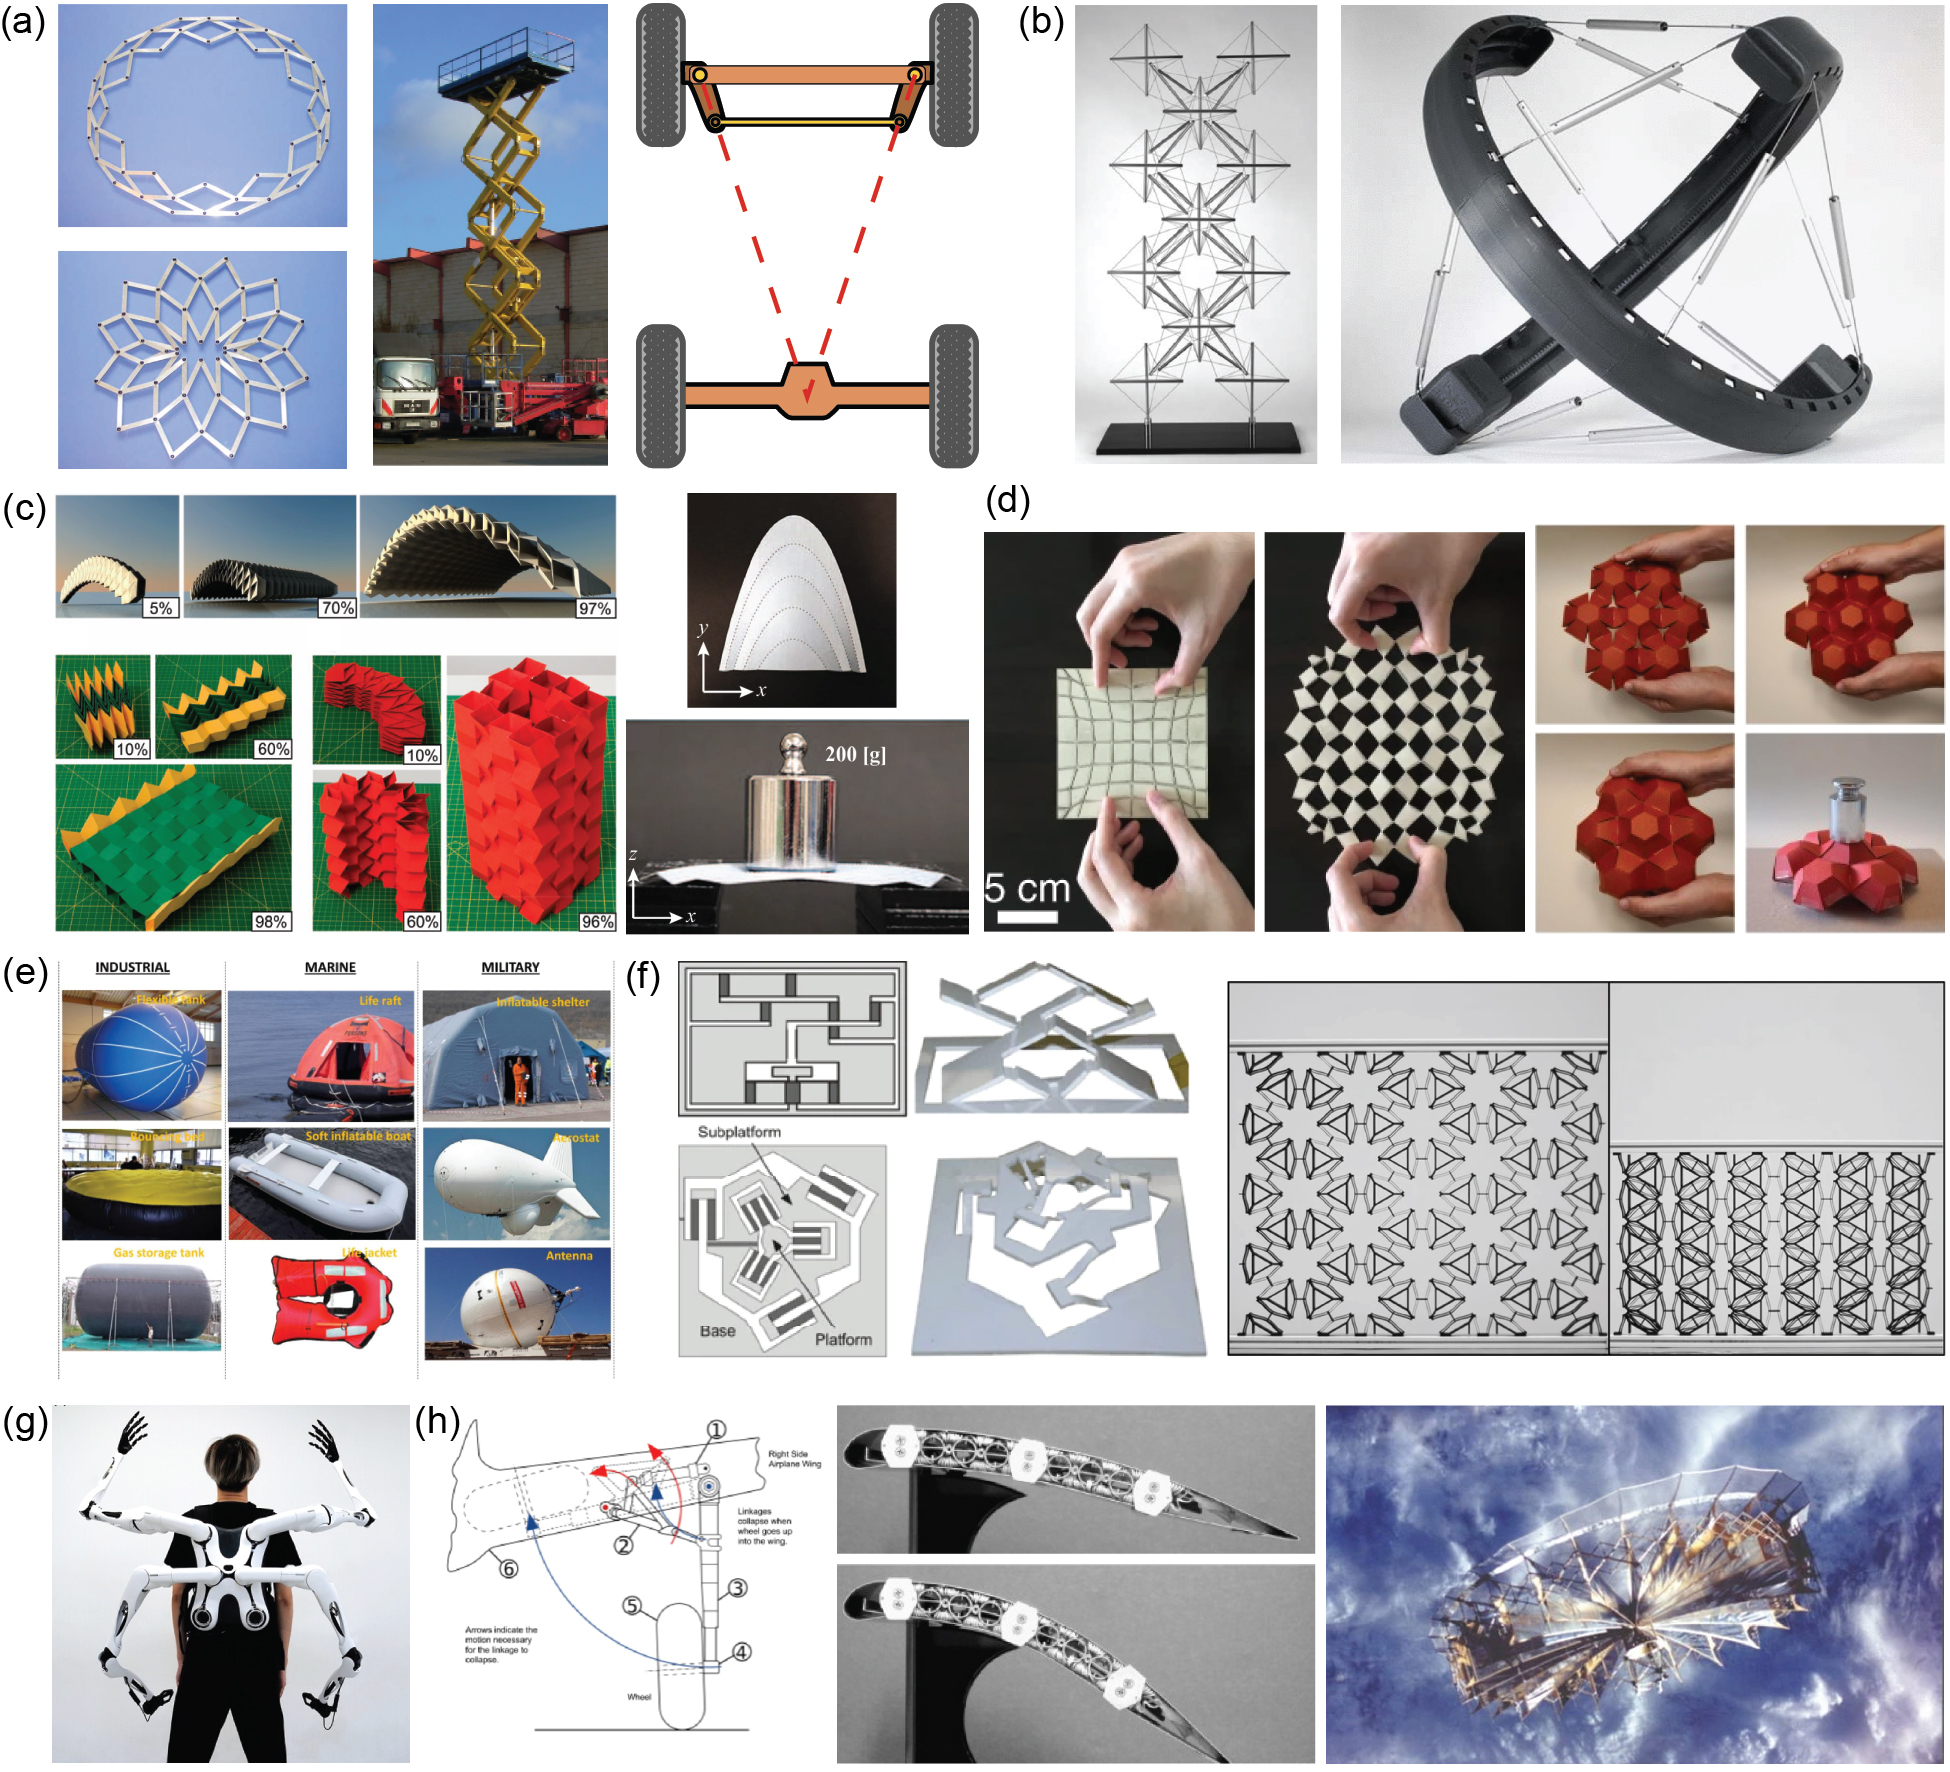
\includegraphics[width=\textwidth]{01-figures/01-01-reconfigurable-structure-examples.jpg}
  \caption{Examples of reconfigurable systems across engineering disciplines. (a) Bar-linked mechanisms: Hoberman linkage~\cite{you2007motion} (left, licensed under CC BY-NC-ND 3.0.), Scissor lift~\cite{knapper2006scissorlift} (middle, licensed under CC BY-SA 2.0 Germany) and Ackermann steering linkage~\cite{bromskloss2010ackermann} (right, licensed under CC BY-SA 3.0); (b) Tensegrity structures: planar tensegrity mast~\cite{snelson2012art} (left, adapted with permission from Sage Publications) and sperical tensegrity robot~\cite{bohm2016spherical} (Copyright \copyright{} 2016, IEEE); (c) Origami tubes for stiff columns, bridges and domes~\cite{filipov2015origami} (left) and curved-crease origami~\cite{woodruff2021curved} (right, adapted with permission from Springer Nature); (d) Kirigami systems: planar auxetic kirigami~\cite{choi2019programming} (left, adapted with permission from Springer Nature) and pop-up kirigami domes~\cite{redoutey2021pop} (right, adapted with permission from Elsevier); (e) Membrane based inflatable systems~\cite{mandlekar2022review} (licensed under CC BY-NC-ND 4.0); (f) Compliant mechanisms~\cite{howell2013compliant} (adapted with permission from Springer Nature) and multistable metamaterials~\cite{zhang2019energy} (licensed under CC BY 4.0); (g) Robotic arms~\cite{yamamura2023social} (licensed under CC BY 4.0); and (h) Aerospace systems: aircraft landing gear~\cite{dtom2009landinggear} (left), shape morphing wings~\cite{sofla2010shape} (middle, adapted with permission from Elsevier) and mesh reflector antenna deployed in orbit~\cite{santiago2013advances} (right, adapted with permission from Springer Nature).}\label{fig-reconfigurable-structures}
\end{figure}

The resulting body of literature spans many distinct families of systems. Mechanical linkages, including Scissor mechanism and Ackerman linkage shown in Fig.~\ref{fig-reconfigurable-structures}\,(a), use connected bars and rotational joints to produce prescribed motion, expansion, and controlled deployment. Tensegrity assemblies consist of isolated compressive struts within a network of prestressed tensile tendons. The balance between these compressive and tensile members enables the creation of lightweight, deployable space masts and towers, as shown in Fig.~\ref{fig-reconfigurable-structures}\,(b). Origami-inspired systems use folding of flat sheets along prescribed crease patterns to generate complex, three-dimensional structures. Origami principles help create structures with intricate surface topologies, architected mechanical responses, and enable compact storage, deployment, and reconfigurability, as shown in Fig.~\ref{fig-reconfigurable-structures}\,(c). Kirigami systems extend the idea of origami further by incorporating strategically placed cuts or slits into thin sheets of material. These cuts help generate auxetic behavior, enhanced flexibility, tunable mechanical properties, and large shape transformations that are difficult to achieve solely through folding, as shown in Fig.~\ref{fig-reconfigurable-structures}\,(d). Pneumatic and membrane-based structures use thin flexible sheets that gain shape and stiffness through internal pressure, prestress, or supporting boundary elements, as shown in Fig.~\ref{fig-reconfigurable-structures}\,(e). Compliant, multistable, and metamaterial systems use elastic instabilities and geometric nonlinearities to program motion, dissipate energy from external loads, or maintain multiple stable states, as shown in Fig.~\ref{fig-reconfigurable-structures}\,(f). Robotic and aerospace systems combine structural components with actuation, sensing, and control to interact with their environment, as shown in Fig.~\ref{fig-reconfigurable-structures}\,(g) and (h).

Despite significant progress, incorporating deployable and reconfigurable systems into conventional large-scale load-bearing structures remains challenging. Civil structures must satisfy strict requirements for stiffness, strength, stability, constructability, reliable connections, and predictable load transfer under prescribed loading conditions. Many reconfigurable systems provide effective mechanisms for shape change, but their changing geometry, complex joints, and material assumptions pose challenges during large-scale implementation. For instance, origami-inspired systems offer powerful ways to transform flat sheets into complex three-dimensional forms. However, at large scales, the thin-sheet mechanics of origami must be adapted to incorporate finite-thickness panels to ensure robust load transfer between components. Even with thickness-accommodation strategies, these systems can develop unintended moments, localized strains, and complex hinge behavior along creases. Compliant mechanisms, multistable systems, and metamaterials provide useful strategies for programmed deformation and energy absorption from external loads. However, many remain tied to small-scale architectures, specialized materials, or unit-cell-level behavior, which do not directly translate to large structural assemblies with conventional members, joints, and supports. Thus, existing systems offer many principles for creating deployable and reconfigurable systems, but far fewer methods for incorporating those principles into established structural topologies that engineers already understand and trust. The next section uses this distinction to define the specific research problem addressed in this dissertation.

\section{Problem Statement: Integrating Reconfigurability into Existing Structural Forms}\label{sec-problem-statement}
The preceding section shows that reconfigurable systems have been studied across many fields. However, many of these systems are designed with a bottom-up philosophy, in which the unit cell is repeated to create a larger system. This dissertation considers the inverse problem of introducing reconfigurability into an existing structural topology without losing the structural function that made the original topology useful.

The central gap is the lack of generalized frameworks for transforming existing structural topologies into reconfigurable systems. Conventional structures such as trusses, frames, and hulls are typically designed to withstand prescribed loads in a fixed configuration. In contrast, reconfigurable systems must satisfy two coupled requirements: they must move between useful configurations and retain predictable mechanical behavior during and after reconfiguration. Existing studies often address one of these requirements in isolation. Mechanism-based studies emphasize motion, while conventional structural design emphasizes load resistance. The unresolved problem is how to combine these requirements in a systematic way.

This gap has three parts. First, there is a need for design methods that begin with conventional structural topologies, rather than with specialized reconfigurable mechanisms. Second, there is a need for analysis tools that can capture the kinematics, load demands, and stability of the resulting systems through large geometric changes. Third, there is a need to understand how added mechanical features, such as rotational stiffness and nonlinear hinge behavior, can turn reconfiguration from a geometric capability into a functional structural response.

We address this broad problem in the context of two structural systems in this dissertation. The primary focus is on truss systems due to their simple and well-defined geometry, connectivity, and load paths. This makes trusses an appropriate platform for studying how static structural topologies can be transformed into reconfigurable systems. The dissertation then extends this broader philosophy to ship hulls, where curved origami principles are used to introduce compact storage, rapid deployment, and on-demand shape-morphing behavior within an established hull form. These two contexts differ in geometry and application. However, they share a common objective: to move from isolated reconfigurable mechanisms to functional reconfigurable structural systems.

\section{Objectives of the dissertation}\label{01-sec-objectives}
This dissertation addresses the central gap identified in the previous section through four objectives.

\noindent{}\textbf{Objective 1: Develop a framework for transforming static trusses into reconfigurable systems.}\\
We develop a framework for transforming static truss designs into reconfigurable systems using principles of planar quadrilateral linkages. The framework introduces kinematic degrees of freedom into selected truss units, enabling the transformed systems to change shape while preserving the primary load paths, stiffness, and peak load capacity of the original designs. We also develop fabrication strategies that allow the transformed systems to deploy as intended without member interference or loss of strength due to out-of-plane moments.

\noindent{}\textbf{Objective 2: Develop computational tools for kinematic and mechanical analysis.}\\
We develop computational tools to evaluate the kinematic and structural response of the reconfigurable trusses. The kinematic tool uses a sequential actuation framework to simulate deployment paths and quantify the packing efficiency of the transformed systems. The structural tool uses a geometric nonlinear analysis framework with axial bar and torsional spring elements to evaluate actuation load demands, behavior during load reversal, and structural response during large deformations.

\noindent{}\textbf{Objective 3: Incorporate programmed hinge behavior into reconfigurable trusses for functional applications.}
We develop programmed rotational hinges that introduce prescribed nonlinear moment-rotation behavior into reconfigurable truss systems. This objective combines a physical hinge design based on magnetic interactions between alternating-polarity magnets with nonlinear torsional spring models that capture bistable and multistable rotational responses. We show that these programmed hinges can assign multiple stable states to independent degrees of freedom in reconfigurable trusses, enabling functional applications such as reusable impact absorption infrastructure.

\noindent{}\textbf{Objective 4: Broaden the framework beyond civil truss systems through curved-crease origami hulls.}\\
We extend the dissertation's philosophy beyond civil structures by using curved-crease origami principles to obtain shape-morphing ship hulls. This objective develops flat-foldable and rapidly deployable hull systems that match conventional planing hull geometries and morph shape for on-demand tunability of hydrodynamic performance. Through this extension, we show that reconfigurability can also be used to rethink established structural forms in naval architecture to achieve functional benefits, such as adaptable hydrodynamic performance.

\section{Organization of the Dissertation}\label{01-sec-organization}
The dissertation is organized as follows to address the objectives described in the previous section:

\textbf{Chapter~\ref{chapter-02}} introduces a method for transforming static trusses into reconfigurable systems. This method uses Grahsof's flat-foldability criterion for planar quadrilateral linkages to strategically introduce a new node in every triangular unit of a given truss. These added nodes convert triangular units into flat-foldable quadrilateral linkages, thereby introducing kinematic degrees of freedom that enable global reconfigurability. A general workflow is presented for applying these transformations to most single-chorded truss designs, and it is supported by a sequential kinematic analysis framework to study the deployment behavior of the resulting systems. This workflow is first demonstrated on traditional truss designs and then extended to topology-optimized trusses with arbitrary geometries, to highlight its broader applicability. The chapter also presents experimental structural analysis of proof-of-concept prototypes to demonstrate fabrication feasibility and to show that the transformed systems retain load-bearing capacity and stiffness of the original designs.

\textbf{Chapter~\ref{chapter-03}} develops a Three-node Torsional Spring (3NTS) element to introduce rotational stiffness at the folding joints of the reconfigurable trusses developed in Chapter~\ref{chapter-02}. The chapter presents a first-principles mathematical formulation of a torsional coil spring element and its implementation within a nonlinear structural solver. The formulation is validated against analytical solutions for two benchmark examples, demonstrating its ability to capture structural instabilities associated with elastic buckling. The chapter then shows how torsional springs can be integrated into reconfigurable trusses to provide functional benefits such as resistance to load reversal, controlled path-dependent deployment, and energy absorption under external loading.

\textbf{Chapter~\ref{chapter-04}} extends the 3NTS formulation from Chapter~\ref{chapter-03} by introducing hinge-level nonlinear constitutive models for bounded rotation, magnetic multistability, and idealized bistability. These models enable the simulation of programmable mechanical response in reconfigurable trusses, including sequential deployment and path-dependent multistability. This capability establishes a foundation for future functional applications of reconfigurable trusses such as reusable infrastructure for impact-energy management.

\textbf{Chapter~\ref{chapter-05}} broadens the perspective of the dissertation by extending the transformation of static structural topology beyond civil engineering and into naval architecture. In this chapter, the focus shifts from reconfigurable truss systems to shape-morphing hull structures inspired by curved-crease origami. The chapter develops curved-crease-origami-inspired planing hulls that can be deployed rapidly from flat sheets, match the shape and therefore, hydrodynamics of conventional planing hulls, and utilize active folding to change shape and tune hydrodynamic performance of the hull on demand. A proof-of-concept prototype is also presented, together with a discussion of the steps required for real-world implementation.

\textbf{Chapter~\ref{chapter-06}} summarizes the main contributions of the dissertation, discusses its limitations, and outlines directions for future research.

Three appendices are included to provide additional background for the analytical tools and methods used throughout the dissertation.

\textbf{Appendix~\ref{01-appendix-seq-kinematics}} presents the mathematical formulation for the positional analysis of planar quadrilateral linkages, which serves as the basis of the sequential kinematic analysis framework used to study deployment of reconfigurable trusses. This appendix also includes the positional analysis of the special six-bar linkage case discussed in Chapter~\ref{chapter-02}, together with a note on interpreting the percentage of actuation of each kinematic degree of freedom in the reconfigurable truss systems.

\textbf{Appendix~\ref{02-appendix-truss-videos}} contains the supplementary videos of fabricated reconfigurable truss prototypes and their load-tests discussed in Chapter~\ref{chapter-02}, to demonstrate failure type and load-carrying capacities.

\textbf{Appendix~\ref{03-appendix-powersea}} describes the theoretical basis of the Powersea software used for the hydrodynamic analyses of planing hulls in Chapter~\ref{chapter-05}. This appendix briefly outlines the \textit{low-aspect-ratio strip theory} used in the software, states the key assumptions, and explains why this approach is suitable for comparative hydrodynamic studies of curved-crease origami and conventional planing hulls.
\chapter{Reconfigurable trusses}
\label{chpt-reconfigurable-trusses}
\chapter{Torsional springs}
\label{chpt-torsional-springs}
\chapter{Programmable Hinge Mechanics for Functional Reconfigurable Trusses}\label{chapter-04}


\section{Introduction}\label{04-sec-functional-intro}
The remainder of the chapter is organized as follows. Section~\ref{04-sec-bounded-rotation} introduces an enhanced formulation of the torsional spring that limits its deformation range and enables study of sequential folding of kinematic degrees of freedom of the reconfigurable truss. Next, Section~\ref{04-sec-multistable-hinge} introduces a multistable torsional hinge design which employs magnetic interaction to achieve multiple stable states. This section also develops a computational model of the magnetic multistable hinge building on the 3NTS model. Section~\ref{04-sec-bistable-spring} introduces a way to model bistable behavior into the 3NTS element and demonstrates reconfigurable trusses with more than one degree of freedom exhibit multiple stable states based on 2 stable states per kinematic degree of freedom. Section~\ref{04-sec-discussion} presents a discussion on the possible applications of the analysis tools and the potential applications the nonlinear hinge modeling enables. Finally, the concluding remarks are presented in Seciton~\ref{04-sec-conclusion}.

\section{Modeling Bounded Rotation in Torsional Spring Hinges}\label{04-sec-bounded-rotation}
This section builds on the Three-Node Torsional Spring (3NTS) element from Chapter~\ref{chapter-03} to enforce limits on the angular rotation of the joints. The enhanced constitutive law preserves the linear spring response within the intended operating range and introduces nonlinear stiffening near the deformation limits. This bounded response prevents inadmissible hinge rotations and enables the analysis of sequential folding, locking, and load redistribution in reconfigurable trusses.

\subsection{Enhanced Torsional Spring Constitutive Law}\label{04-subsec-enhanced-spring}
The Three-Node Torsional Spring (3NTS) element was originally formulated using a linear torsional spring constitutive law. In this formulation, the spring deformation is described by the relative angle \(\alpha\) defined over the interval \([0,~2\pi)\). The spring's restoring moment is proportional to the difference between the current relative angle \(\alpha\) and the rest angle \(\alpha_0\). While this formulation works as long as \(0 \le \alpha < 2\pi\), numerical issues arise when the spring undergoes large rotations associated with self-overlap of the connected bars. Since \(\alpha\) is evaluated over [\(0,~2\pi\)), the computed angle wraps from \(2\pi\) to 0 when the rotation exceeds this range. This behavior produces a sudden discontinuity in the computed spring deformation, leading to inconsistent restoring moments and tangent stiffness with the actual deformation path.

This numerical issue is also inconsistent with the observed physical behavior of the reconfigurable truss systems discussed in this dissertation. In these systems, the bars connected to a torsional spring do not overlap each other during reconfiguration. The fabrication techniques and kinematics of the truss physically limit the allowable rotation at each folding joint, as discussed in Chapter~\ref{chapter-02} (see Fig.~\ref{fig-warren-test}\,(c)). Furthermore, relative angles near 0 or \(2\pi\) correspond to a fully actuated degree of freedom, where the truss has reached its most compact configuration. Rotation of the spring joint beyond this state becomes meaningless. Therefore, rotations beyond 0 or \(2\pi\) do not represent the intended deformation range of the torsional springs in the physical structure. This motivates restricting the admissible angular range of the torsional spring.

To address the numerical issue and ensure that the spring model captures a realistic range of deformation for the folding joints, the constitutive law of the 3NTS element is modified using the concepts inspired by the bar-and-hinge model~\cite{liu2017merlin}. The modified formulation restricts the admissible deformation range of the spring by introducing nonlinear stiffening near the extreme deformation limits. This stiffening acts as a smooth mechanical stop, providing increasing resistance as the joint approaches its allowable rotation limit. The modified formulation, referred to as the \textit{Enhanced Spring Law}, preserves the original linear response near the rest configuration while creating high-energy barriers at the lower and upper deformation limits.

The enhanced spring law introduces three additional parameters to define the admissible deformation limits of the spring. The parameter, \(\delta\), defines the minimum allowable relative angle between the two connected members. Therefore, the lower admissible deformation limit of the spring becomes \(\delta\). By symmetry, the upper admissible limit becomes \(2\pi-\delta\). The parameters \(\alpha_1\) and \(\alpha_2\) define the lower and upper threshold angles, respectively, at which the spring response transitions from the linear to the nonlinear stiffening regime. These parameters satisfy the following relationship: \(0 \le \delta < \alpha_1 < \alpha_0 < \alpha_2 < 2\pi-\delta \le 2\pi\). Thus, the interval [\(\alpha_1,~\alpha_2\)] represents the nominal operating range of the spring. Within this range, the enhanced law is identical to the original linear torsional spring law. The intervals (\(\delta,~\alpha_1\)) and (\(\alpha_2,~2\pi-\delta\)), on the other hand, represent the nonlinear stiffening regions near the lower and upper deformation limits, respectively.

\begin{figure}[!ht]
  \centering
  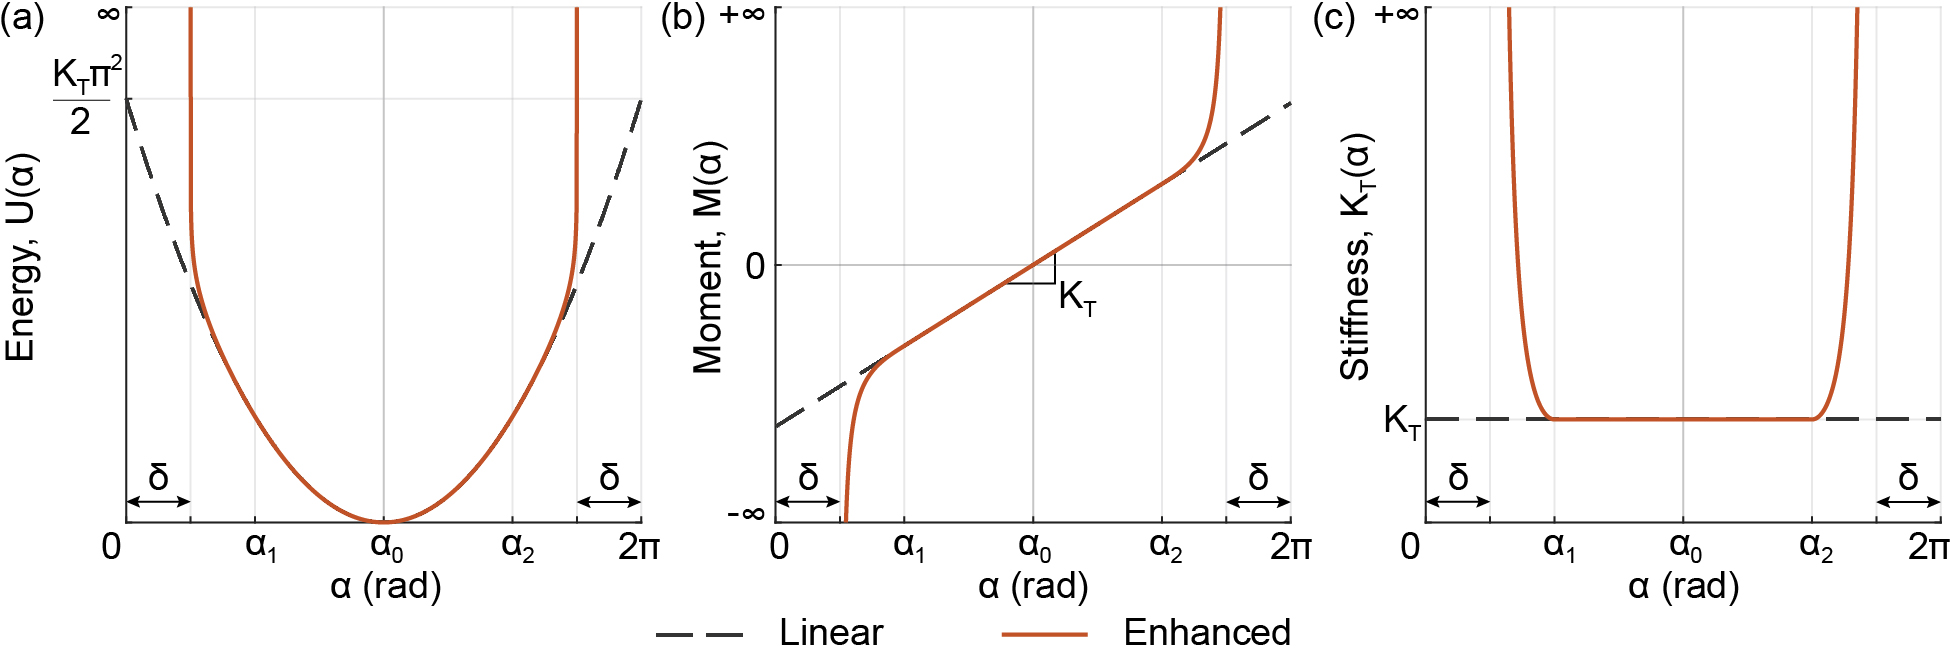
\includegraphics[width=\textwidth]{01-figures/04-01-spring-law-comparison.jpg}
  \caption{Comparison between the original linear torsional spring law (dashed line) and the enhanced spring law (solid line): (a) strain energy; (b) restoring moment; and (c) tangent stiffness as functions of the relative angle \(\alpha\). Here, \(\alpha_0\) is the rest angle, \(\alpha_1\) and \(\alpha_2\) are the lower and upper threshold angles where the spring response changes from linear to nonlinear stiffening, respectively, and \(\delta\) and \(2\pi-\delta\) are the lower and upper admissible deformation limits, respectively.}\label{fig-spring-law-comparison}
\end{figure}

The strain energy, U(\(\alpha\)), of the enhanced spring law is defined as
\begin{flalign}
\quad{}U(\alpha)&=
\begin{cases}
\frac12 K_T(\alpha_0-\alpha_1)^2
+ K_T(\alpha_0-\alpha_1)(\alpha_1-\alpha)
\\- \frac{4K_T(\alpha_1-\delta)^2}{\pi^2}
\ln\!\left|\cos\!\left(\frac{\pi(\alpha_1-\alpha)}{2(\alpha_1-\delta)}\right)\right|, & \alpha < \alpha_1 \\[24pt]
\frac12 K_T(\alpha-\alpha_0)^2, & \alpha_1 \le \alpha \le \alpha_2 \\[24pt]
\frac12 K_T(\alpha_2-\alpha_0)^2
+ K_T(\alpha_2-\alpha_0)(\alpha-\alpha_2)
\\- \frac{4K_T((2\pi-\delta)-\alpha_2)^2}{\pi^2}
\ln\!\left|\cos\!\left(\frac{\pi(\alpha-\alpha_2)}{2((2\pi-\delta)-\alpha_2)}\right)\right|, & \alpha > \alpha_2
\end{cases}&\label{eq-enhanced-energy}
\end{flalign}

The restoring moment of the enhanced spring is obtained as the first derivative of the strain energy with respect to the relative angle \(\alpha\) as
\begin{flalign}
\quad{}M(\alpha)&=
\begin{cases}
K_T(\alpha_1-\alpha_0) + \dfrac{2K_T(\alpha_1-\delta)}{\pi}\tan\Bigg(\frac{\pi(\alpha-\alpha_1)}{2(\alpha_1-\delta)}\Bigg),
& \alpha < \alpha_1 \\[24pt]
K_T(\alpha-\alpha_0),
& \alpha_1 \le \alpha \le \alpha_2 \\[24pt]
K_T(\alpha_2-\alpha_0) + \dfrac{2K_T(2\pi-\delta-\alpha_2)}{\pi}\tan\Bigg(\frac{\pi(\alpha-\alpha_2)}{2(2\pi-\delta-\alpha_2)}\Bigg),
& \alpha > \alpha_2
\end{cases}&\label{eq-enhanced-moment}
\end{flalign}

The corresponding tangent rotational stiffness of the enhanced spring is obtained as the derivative of the restoring moment with respect to \(\alpha\) as
\begin{flalign}
\quad{}K_T(\alpha)&=
\begin{cases}
K_T\,\sec^2\Bigg(\frac{\pi(\alpha-\alpha_1)}{2(\alpha_1-\delta)}\Bigg), & \alpha < \alpha_1\\[24pt]
K_T,& \alpha_1 \le \alpha \le \alpha_2
\\[24pt]
K_T\,\sec^2\Bigg(\frac{\pi(\alpha-\alpha_2)}{2((2\pi-\delta)-\alpha_2)}\Bigg), & \alpha > \alpha_2
\end{cases} & \label{eq-enhanced-stiffness}
\end{flalign}

Figure~\ref{fig-spring-law-comparison}\,(a-c) compares the original linear torsional spring law (dashed line) with the enhanced spring law (solid line) in terms of strain energy, restoring moment, and tangent rotational stiffness. It is important to note that the values of \(\delta\), \(\alpha_1\), and \(\alpha_2\) used in Fig.~\ref{fig-spring-law-comparison} are chosen for visual representation only and are not up to scale. 

The spring response can be divided into three regions. Firstly, when \(\alpha_1 \le \alpha \le \alpha_2\), the enhanced law reduces to the original 3NTS constitutive law. The tangent stiffness is constant and equal to \(K_\textrm{T}\), the restoring moment varies linearly with \(\alpha-\alpha_0\), and the strain energy varies quadratically with \(\alpha-\alpha_0\). The energy minimum occurs at \(\alpha=\alpha_0\), where the restoring moment is zero. Thus, the enhanced law does not alter the spring response in the intended operating range. In the lower stiffening region, where \(\delta < \alpha < \alpha_1\), the spring stiffens as the relative angle decreases below \(\alpha_1\). The tangent stiffness increases according to a secant-squared function and tends to infinity as \(\alpha \rightarrow \delta^+\). The restoring moment becomes increasingly negative. This moment resists further closure of the joint. The strain energy also grows rapidly as the lower admissible limit is approached. In the upper stiffening region, where \(\alpha_2 < \alpha < 2\pi-\delta\), the spring stiffens as the relative angle increases beyond \(\alpha_2\). The tangent stiffness again tends to infinity, now as \(\alpha \rightarrow (2\pi-\delta)^-\). The restoring moment becomes increasingly positive. This moment resists further deformation of the joint. The strain energy also grows rapidly near the upper admissible limit.

\subsection{Path-dependent loading and Sequential Folding Enabled by Enhanced Torsional Spring}\label{04-subsec-deployment-path}

The enhanced spring law formulated in the previous subsection allows the 3NTS element to model large rotations while enforcing prescribed angular limits. This capability is important for reconfigurable trusses with multiple independent kinematic degrees of freedom. In such systems, individual units may fold, lock, or remain active at different stages of deformation. The enhanced spring law allows the simulation of these transitions without numerical failure caused by angle wrapping, spring overlap, or physically inadmissible rotations. This subsection demonstrates these capabilities using two examples.

The first example is the stacked square-linkage truss shown in Fig.~\ref{fig-deployment-path}\,(a). The structure consists of two vertically stacked square units. Each unit is a special case of a six-bar linkage, formed by a square frame and two diagonal bars with a rotational joint at their connection. The joint at the midpoint of each diagonal is modeled using the enhanced torsional spring. Each unit, therefore, contributes one independent kinematic degree of freedom to the structure.

The structure is approximately 2~m tall. Each non-diagonal member has a length of 1~m. The bars have an elastic modulus \(E = 3\times10^9~\text{Pa}\) and a cross-sectional area \(A = 0.5~\text{m}^2\). Each torsional spring has a linear-regime stiffness \(K_T = 10~\text{Nm/rad}\). A geometric imperfection of \(10^\circ\) is assigned to each torsional spring joint to simulate buckling deformation of the diagonal bars. The admissible rotation range is bounded between \(15^\circ\) and \(345^\circ\) and the spring response remains linear between \(30^\circ\) and \(330^\circ\). Outside this interval, the tangent stiffness increases asymptotically as the spring angle approaches the prescribed maximum angular deformation limits. Using the notation from the previous subsection, these enhanced spring law parameters are set to \(\alpha_1 = 30^\circ\), \(\alpha_2 = 330^\circ\), and \(\delta_1 = 15^\circ\).

The load-displacement response of the stacked square-linkage truss is shown in Fig.~\ref{fig-deployment-path}\,(b). At the beginning of loading, both units resist the applied vertical load. The structure carries a load of approximately 180~N before instability develops in the lower unit. After this instability, the load drops as the lower unit folds. The lower unit continues to deform until the relative angle of its torsional spring approaches the lower angular limit of \(15^\circ\). At this stage, the enhanced spring law makes the torsional spring increasingly stiff, preventing any further deformation of the lower unit.

After the lower unit locks, additional load on the system is redistributed and transferred to the upper unit. The load then increases again, leading to a second instability in the upper unit. The upper unit folds like the lower unit until its torsional spring also approaches the lower angular limit. Once both the units are locked, any further increase of load on the structure is resisted by a combination of the axial deformation of the bars and the extremely stiff torsional springs. This produces the final steep increase in the load-displacement curve near \(\Delta = 1.6~\text{m}\), as shown in Fig.~\ref{fig-deployment-path}\,(b).

\begin{figure}[!ht]
  \centering
  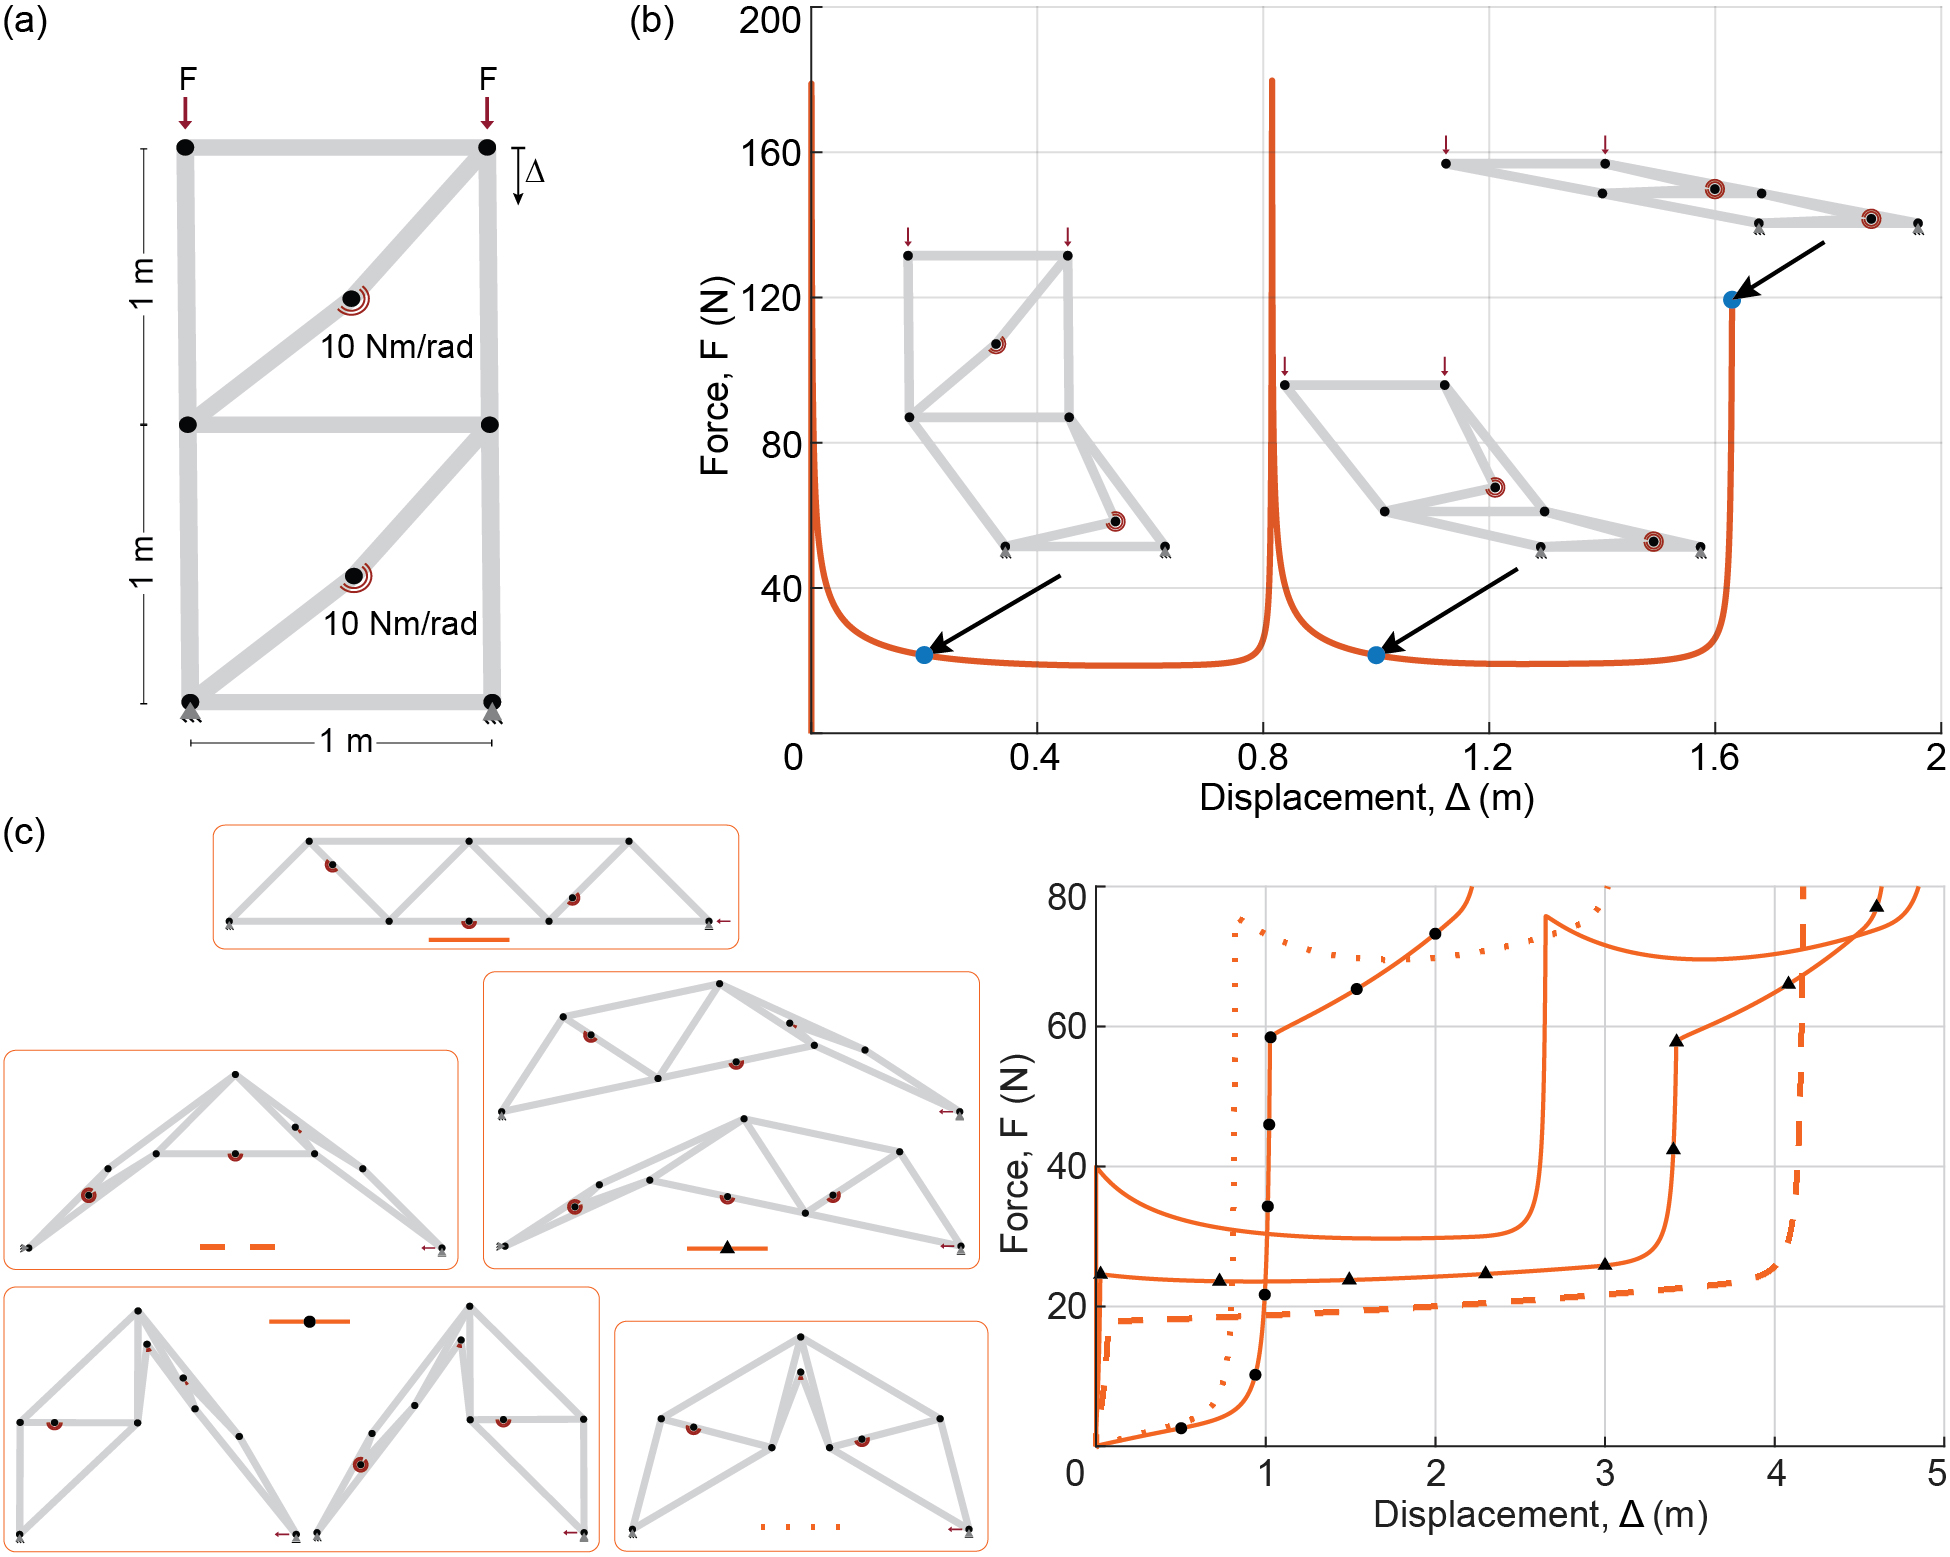
\includegraphics[width=\textwidth]{01-figures/04-02-path-analysis.jpg}
  \caption{(a) Vertically stacked square-linkage truss with two independent folding units under compression. Each unit contains an enhanced torsional spring at the midpoint of the diagonal member; (b) Load-displacement response showing sequential development of instability, folding, and locking of the structure's kinematic units; (c) Reconfigurable Warren truss configurations produced by folding different combinations of its independent kinematic units; (d) Load-displacement responses for folding various Warren truss configurations to the same compact state. The intermediate force demand depends on the folding path, even when the maximum force required to fold the entire structure is the same.}\label{fig-deployment-path}
\end{figure}

This example illustrates the main advantage of the enhanced spring law. The formulation can capture sequential folding, locking, and load redistribution in a reconfigurable truss with multiple independent kinematic degrees of freedom. A conventional linear torsional spring cannot represent this behavior reliably because it does not impose a physical angular range. The enhanced law therefore provides a way to study collapse sequences, deployment sequences, and actuation paths in systems in which different units activate at different stages of deformation.

The second example considers the reconfigurable Warren truss and its various configurations shown in Fig.~\ref{fig-deployment-path}\,(c). The truss is 6~m long and 1~m high. The left support is pinned, and the right support is modeled as a roller. Three enhanced torsional springs are placed at the locations marked with red arcs, as shown in Fig.~\ref{fig-deployment-path}\,(c). Since the structure has three independent kinematic degrees of freedom, the structure can occupy several intermediate configurations depending on which units remain folded or open. Excluding symmetric cases, the truss has five unique starting configurations shown in Fig.~\ref{fig-deployment-path}\,(c).

Each configuration is loaded by applying a vertical displacement at the roller support in the negative y-direction. The corresponding load-displacement curves are shown in Fig.~\ref{fig-deployment-path}\,(d). Each torsional spring has a geometric imperfection of \(0.1^\circ\), and the linear-regime torsional stiffness is set at \(K_T = 20~\text{Nm/rad}\).

The results show that all loading paths eventually require approximately 80~N to reach the most compact final state. However, the force demand varies substantially during the intermediate stages of folding. This variation occurs because each starting configuration activates a different set of kinematic degrees of freedom. Some configurations deform through a gradual folding sequence. Others require one or more units to snap through or lock before the remaining units can continue to fold. As individual units reach their angular limits, the enhanced springs restrict further rotation and redirect deformation to the remaining active units.

Therefore, the final compact configuration alone does not define the actuation demand. The required force also depends on the folding path used to reach that configuration. The enhanced torsional spring law makes this path dependence accessible in simulation. It allows the force demand to be evaluated for different deployment or collapse sequences while maintaining physically admissible joint rotations. This capability is useful for designing reconfigurable trusses that must fold in a prescribed order, avoid unintended locking, or minimize actuation forces along a selected kinematic path.

\section{Magnetic Multi-stable Torsional Hinges}\label{04-sec-multistable-hinge}
This section presents a magnetic multistable torsional hinge that uses polarity-dependent interactions between permanent magnets to create multiple stable rotational states. The physical design, fabrication, and reduced-order torque--rotation model are first introduced to characterize the hinge behavior. The multistable hinge response is then incorporated into the 3NTS element formulation, enabling programmable mechanical response in the reconfigurable trusses.

\subsection{Prototype and Reduced-order Simulated Response of a Magnetic Multistable Hinge}\label{04-subsec-magnetic-hinge-prototype}
The magnetic torsional hinge prototype uses polarity-dependent interactions between permanent magnets to create preferred rotational states. The hinge is formed at the joint between two axial members whose ends remain adjacent during rotation. Each member terminates in a circular hub, which provides the mating surface for the magnetic connection, as shown in Fig.~\ref{fig-magnetic-prototype}\,(a). Each hub face contains eight identical N35-grade cylindrical neodymium magnets with a diameter of 6~mm and a thickness of 2~mm. The magnets are seated in individual holes and are equally spaced at 45\(^\circ{}\) intervals around the hinge axis. The center of each magnet lies on a pitch circle with a radius of 13.75~mm. The opposing hub uses the same geometric layout, so corresponding magnets align face-to-face when the two hubs are in selected relative orientations. The exposed poles alternate between north and south around each hub face, and the pole sequence on the opposing hub is arranged so that aligned magnet pairs have opposite-facing poles in the preferred configurations. As the hubs rotate relative to each other, the facing magnet pairs move between attractive and repulsive alignments, producing a periodic magnetic torque and multiple stable rotational states. The hub dimensions and magnet layout are shown in Fig.~\ref{fig-magnetic-prototype}\,(a).

As one hub rotates relative to the other, the facing magnet pairs periodically move between attracting and repelling configurations. Stable states occur at relative rotations where the two magnet arrays form an energetically favorable pole arrangement. For the eight-magnet alternating-polarity pattern used in this prototype, the magnetic layout repeats every \(\pi/2\) radians, resulting in four stable states over one full rotation. Figure~\ref{fig-magnetic-prototype}\,(b, left) shows the 3D-printed hinge components with embedded magnets, and Fig.~\ref{fig-magnetic-prototype}\,(b, right) shows the four stable configurations of the magnetic multistable hinge integrated into a four-bar linkage unit.

\begin{figure}[!ht]
  \centering
  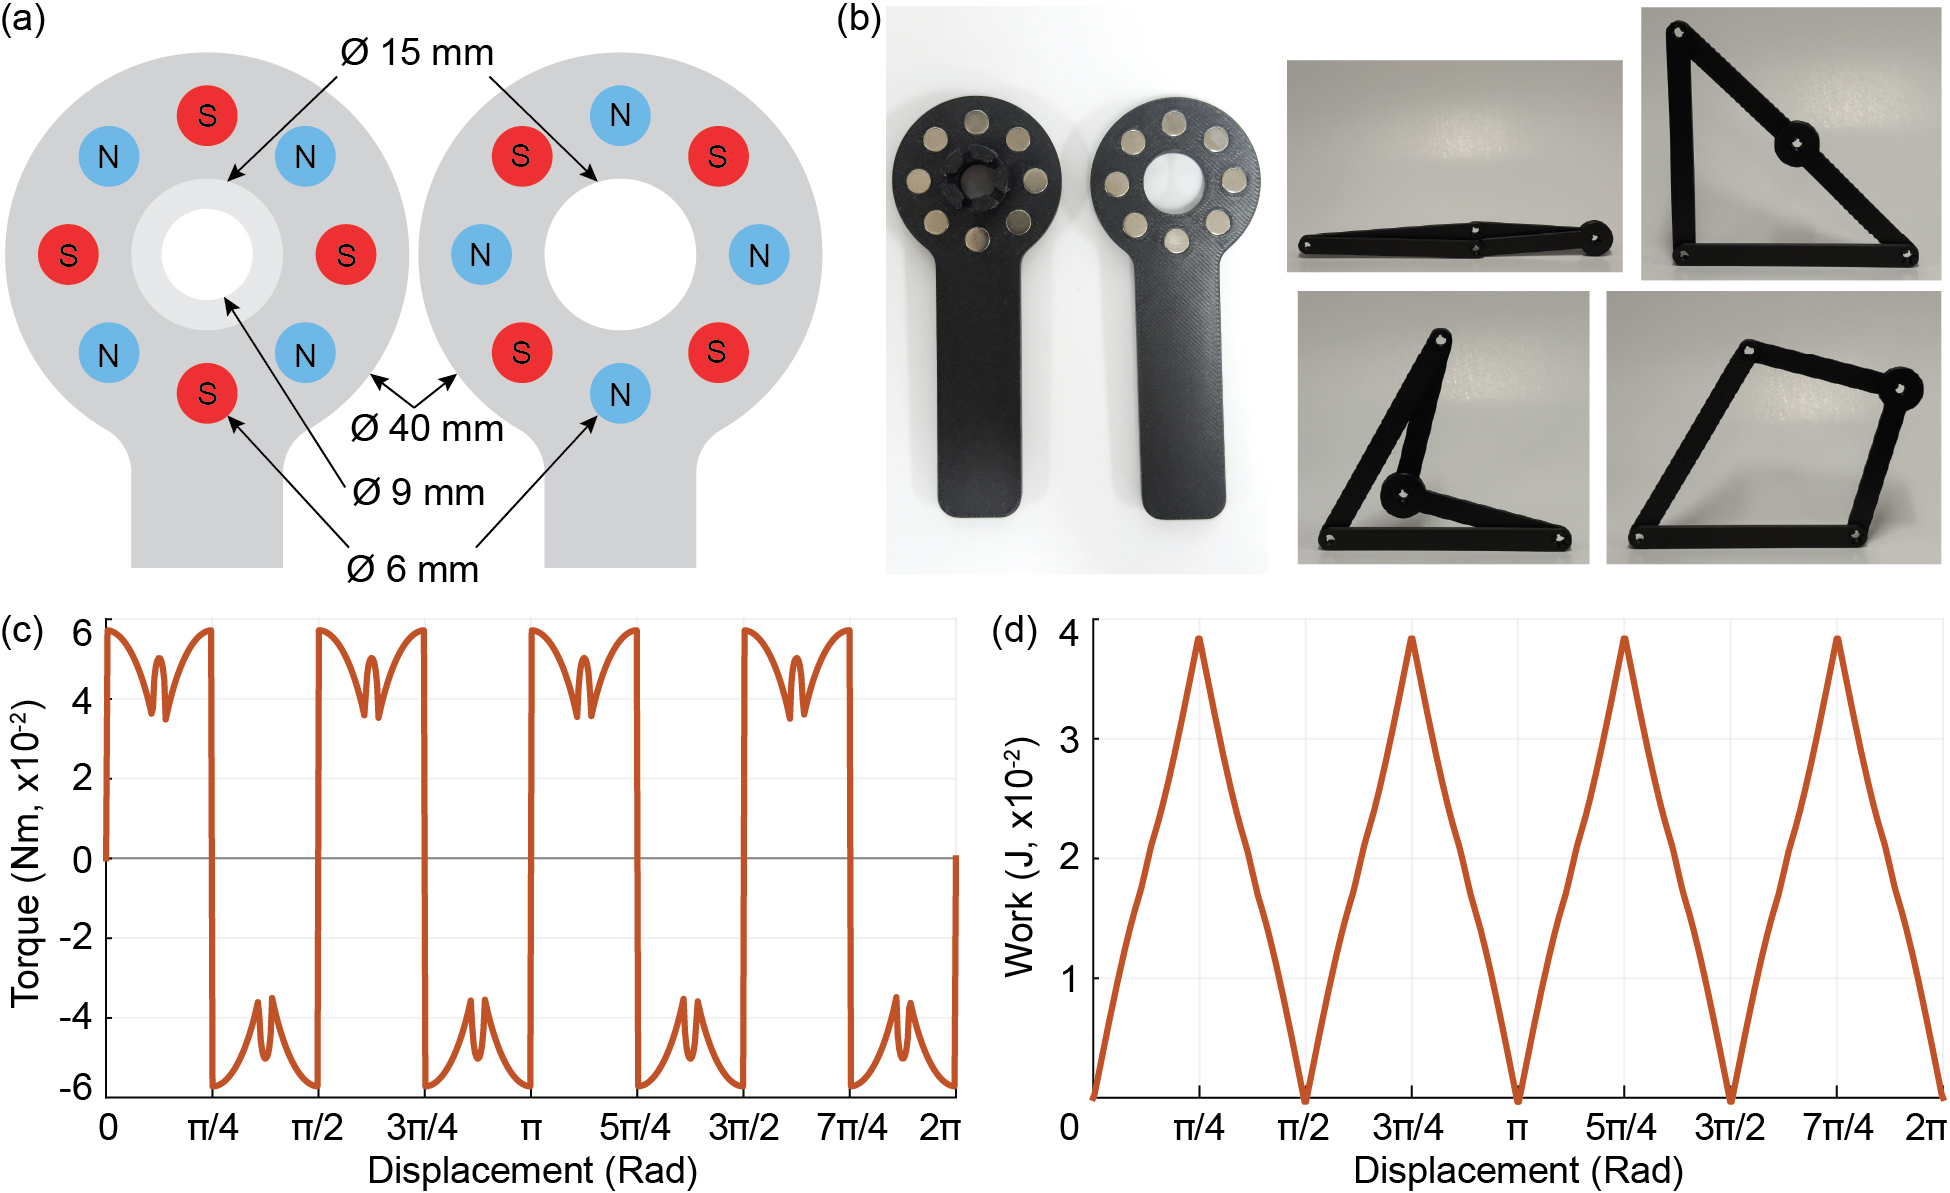
\includegraphics[width=\textwidth]{01-figures/04-03-magnetic-hinge-prototype.jpg}
  \caption{Magnetic multistable torsional hinge prototype: (a) Magnet placement and dimensions of the torsional hinge hub; (b) 3D printed and assembled prototype of a magnetic multistable hinge in a 4-bar linkage unit; Simulated behavior of the magnetic multistable torsional hinge using a reduced-order magnetic interaction model: (c) Torque-displacement, and (d) Work-displacement response over one full rotation.}\label{fig-magnetic-prototype}
\end{figure}

A reduced-order magnetic interaction model is used to estimate the torque required to drive the hinge through multiple stable states and the corresponding work associated with this rotation. The model provides a simple way to interpret the periodic peaks and troughs in the energy landscape produced by the alternating magnet-polarity pattern. The resulting torque-displacement and work–displacement relationships are later used to model multistable hinge behavior in the 3NTS element for multistable reconfigurable truss simulations.

Each magnet is modeled as a cylindrical disc with diameter \(D\), radius \(r=D/2\), thickness \(t\), remanence \(B_r\), and axial gap \(g\) between the magnets. The axial magnetic field at the opposing face is approximated as:
\begin{equation}
B =\frac{B_r}{2}\left[\frac{z_1}{\sqrt{z_1^2+r^2}}-\frac{z_0} {\sqrt{z_0^2+r^2}}\right]
\end{equation}
where, \(z_0 = g\) and \(z_1 = g + t\). The corresponding magnetic pressure is estimated using
\begin{equation}
P = \frac{B^2}{2\mu_0}
\end{equation}
where \(\mu_0 = 4\pi \times 10^{-7}\ \mathrm{N/A^2}\) is the permeability of the free space. The units of \(P\) are N/m\(^2\), which are equivalent to J/m\(^3\). Therefore, the magnetic pressure can be interpreted as an approximate magnetic energy density. In this reduced-order model, the magnetic energy is estimated by multiplying this energy density by the effective interaction volume between the magnets. The force associated with a change in magnet position is then obtained by differentiating the magnetic energy with respect to the corresponding displacement direction.

For the rotating assembly, one hub face is held fixed while the opposing hub face rotates over it. The effective overlap area between the two magnet arrays is denoted by \(A(\theta)\), where \(\theta\) is the angular position of the rotating face of the hub. The total magnetic interaction energy of the system at any given instance then becomes
\begin{equation}
U(\theta) \approx PV(\theta)
\end{equation}
where \(V(\theta)=\ell A(\theta)\) is the effective interaction volume between the two hub faces and \(\ell=t+g\) is the interaction height, taken as the sum of the magnet thickness and axial gap. The torque associated with the magnetic interaction is approximated from the rate of change of the overlap area with respect to the angular displacement  \(\theta\):
\begin{equation}
\tau(\theta) \approx - P \ell \frac{dA}{d\theta}
\end{equation}

The simulated torque required to rotate the magnetic multistable hinge and the corresponding work are shown in Fig.~\ref{fig-magnetic-prototype}\,(c) and (d), respectively. The alternating magnet polarity produces a periodic response with a period of \(\pi/2\) radians, resulting in four repeating regions over one full rotation. In the torque-rotation response, sharp transitions occur from a positive to negative torque as magnet pairs on either face switch between attractive and repulsive configurations. The corresponding work-rotation response forms a periodic energy landscape with four repeated energy wells. The local minima correspond to stable configurations, while the local maxima represent energy barriers between adjacent stable states. These four energy minima are consistent with the stable states observed in the fabricated four-bar linkage prototype.

\subsection{Computational Modeling of Multistable Magnetic Torsional Hinge for Matrix Structural Analysis}\label{04-subsec-magnetic-hinge-model}
\begin{figure}[!ht]
  \centering
  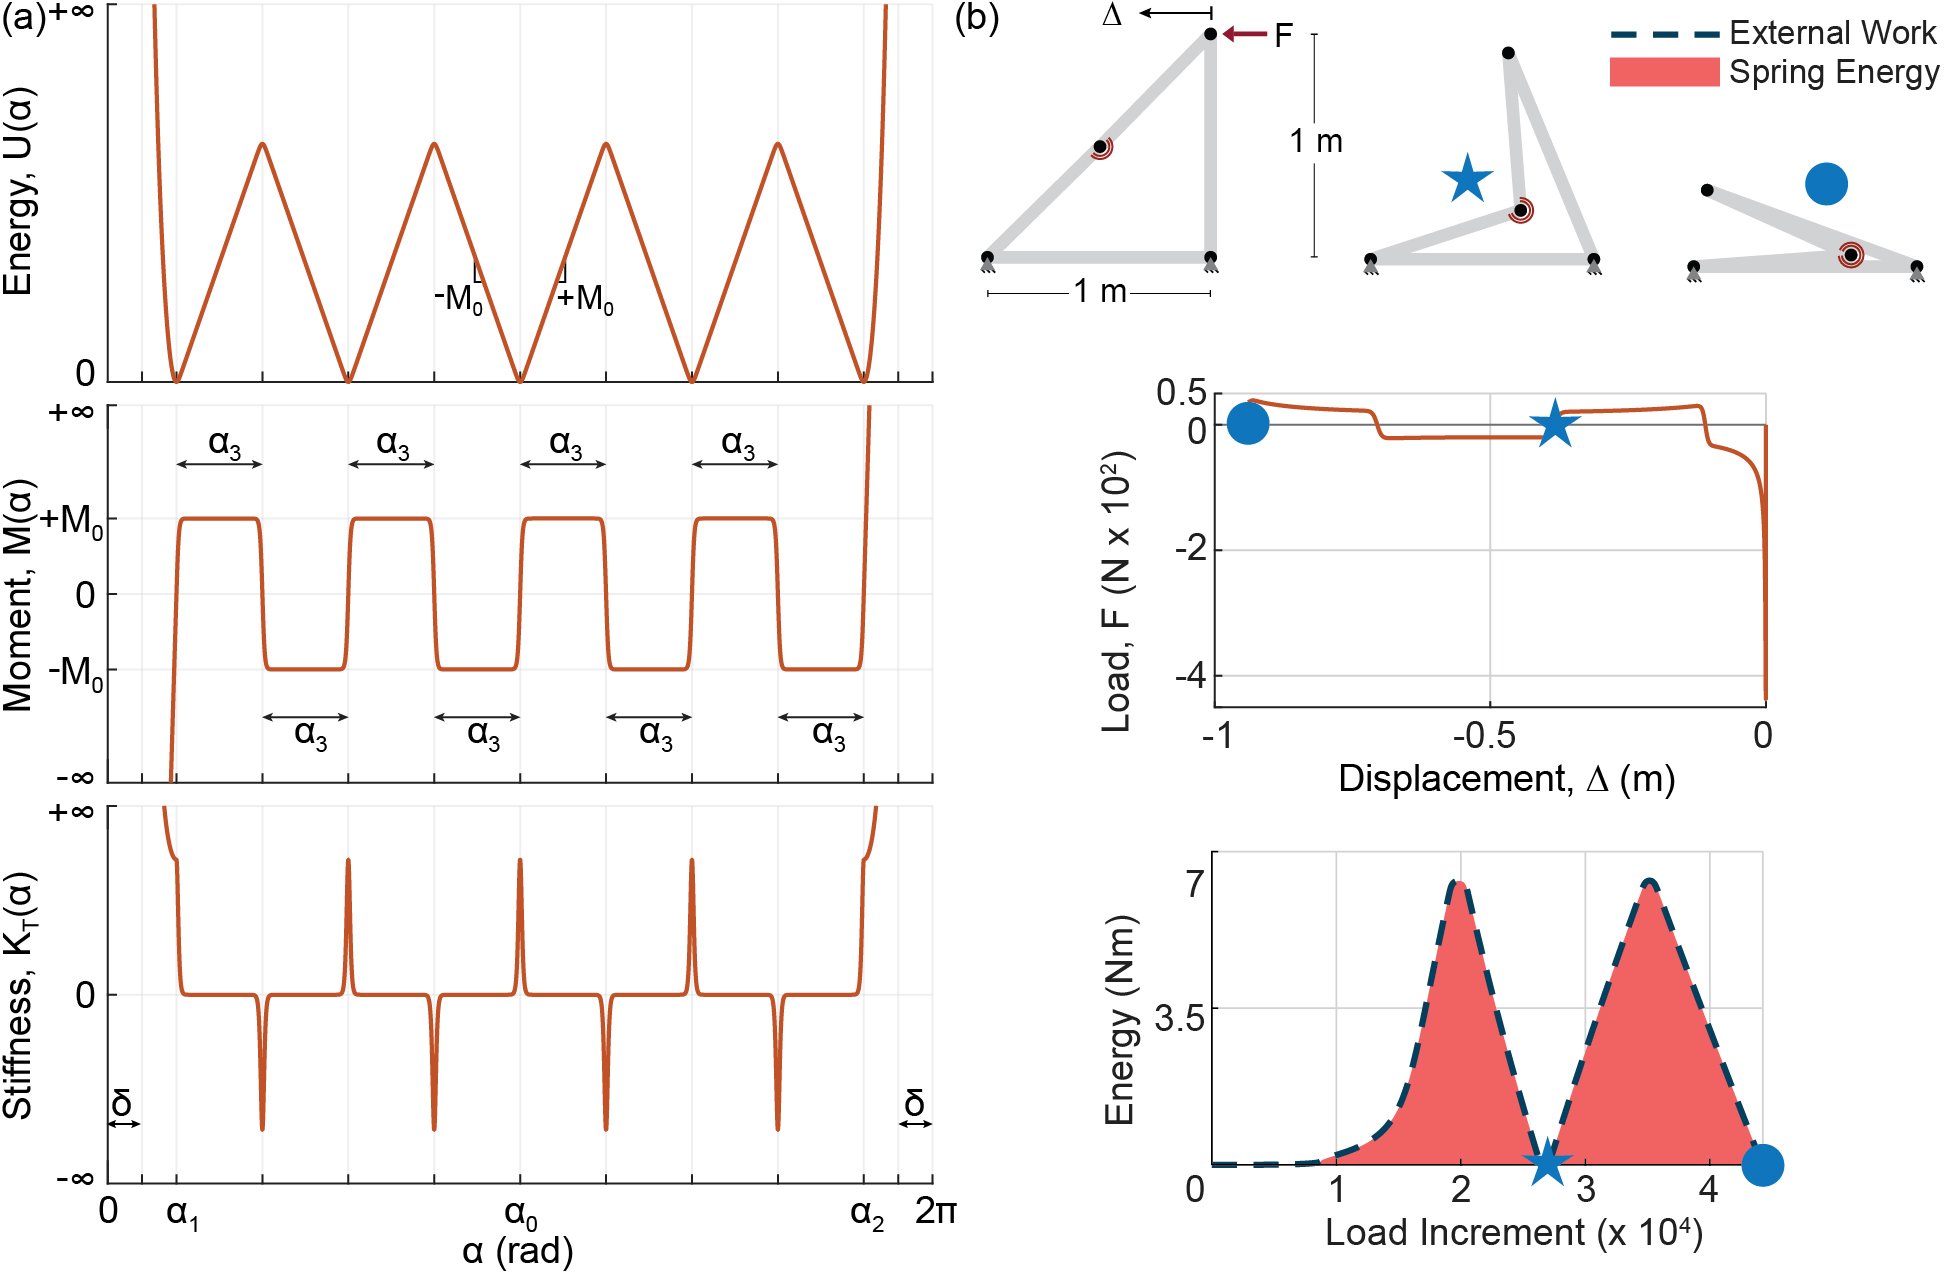
\includegraphics[width=\textwidth]{01-figures/04-04-magnetic-hinge-modeling.jpg}
  \caption{Bistable torsional hinge: (a) Schematic representation of the strain energy (top), restoring moment (middle), and tangent stiffness (bottom) curves for a multistable magnetic torsional hinge with respect to the relative angle of the hinge; (b) Load vs. Displacement (left) and System energy vs. Displacement (right) curves for the buckling of colinear bars in compression fitted with a bistable torsional hinge.}\label{fig-magnetic-hinge}
\end{figure}
Within the central angular interval \(\alpha_1<\alpha<\alpha_2\), the
magnetic multistable hinge is described using the relative rotation
\begin{equation}
\theta=\alpha-\alpha_0,
\label{eq:theta}
\end{equation}
where \(\alpha_0\) is the reference angle. The response outside
\(\alpha_1<\alpha<\alpha_2\) is modeled using the enhanced spring law described
in the preceding section.

The hinge combines a weak linear stiffness with a periodic magnetic
contribution. The two stiffness scales are
\begin{equation}
K_1=\frac{k_0}{10^4},
\qquad
K_2=k_0,
\label{eq:stiffness-scales}
\end{equation}
where \(K_1\) controls the weak background stiffness and \(K_2\) controls the
magnitude of the magnetic contribution. Let \(N=n_{\mathrm{peaks}}\) denote the
number of magnetic periods on each side of \(\theta=0\). The period is
\begin{equation}
p=\frac{\alpha_2-\alpha_0}{N},
\label{eq:period}
\end{equation}
so that, for the symmetric central region,
\begin{equation}
\alpha_1=\alpha_0-Np,
\qquad
\alpha_2=\alpha_0+Np.
\label{eq:symmetric-central-region}
\end{equation}

The smoothing width is
\begin{equation}
\varepsilon=\frac{\pi}{180}\,\varepsilon_{\mathrm{deg}},
\label{eq:smoothing-width}
\end{equation}
where \(\varepsilon_{\mathrm{deg}}\) is specified in degrees. Smaller
\(\varepsilon\) produces sharper magnetic transitions, while larger
\(\varepsilon\) produces smoother transitions.

For each magnetic period, define the local phase coordinate
\(\varphi\in[0,p]\). The three smooth transition functions within a period are
centered at \(\varphi=0\), \(\varphi=p/2\), and \(\varphi=p\). Define
\begin{align}
\mathcal{T}(\varphi)
&=
\tanh\!\left(\frac{\varphi}{\varepsilon}\right)
-\tanh\!\left(\frac{\varphi-\frac{p}{2}}{\varepsilon}\right)
+\tanh\!\left(\frac{\varphi-p}{\varepsilon}\right),
\label{eq:T-shape}\\
\mathcal{S}(\varphi)
&=
\operatorname{sech}^2\!\left(\frac{\varphi}{\varepsilon}\right)
-\operatorname{sech}^2\!\left(\frac{\varphi-\frac{p}{2}}{\varepsilon}\right)
+\operatorname{sech}^2\!\left(\frac{\varphi-p}{\varepsilon}\right).
\label{eq:S-shape}
\end{align}
Here \(\mathcal{T}\) defines the smooth magnetic moment shape within one
period, and \(\mathcal{S}=d\mathcal{T}/d(\varphi/\varepsilon)\) defines the
corresponding stiffness shape.

The energy primitive uses
\begin{equation}
\operatorname{logCosh}(x)
=
|x|+\log\!\left(1+\exp[-2|x|]\right)-\log 2,
\label{eq:logcosh}
\end{equation}
with the constant
\begin{equation}
c_0=
\operatorname{logCosh}(0)
-\operatorname{logCosh}\!\left(-\frac{p}{2\varepsilon}\right)
+\operatorname{logCosh}\!\left(-\frac{p}{\varepsilon}\right).
\label{eq:c0}
\end{equation}
The corresponding dimensionless energy shape is
\begin{equation}
\mathcal{E}(\varphi)
=
\operatorname{logCosh}\!\left(\frac{\varphi}{\varepsilon}\right)
-\operatorname{logCosh}\!\left(\frac{\varphi-\frac{p}{2}}{\varepsilon}\right)
+\operatorname{logCosh}\!\left(\frac{\varphi-p}{\varepsilon}\right)
-c_0.
\label{eq:E-shape}
\end{equation}

For the \(m\)-th magnetic period, where \(m=0,1,\ldots,N-1\), the local phase
coordinate is
\begin{equation}
\varphi_m^+(\theta)=\theta-mp,
\qquad
mp<\theta\le(m+1)p,
\label{eq:positive-phase}
\end{equation}
on the positive side, and
\begin{equation}
\varphi_m^-(\theta)=-\theta-mp,
\qquad
-(m+1)p\le\theta< -mp,
\label{eq:negative-phase}
\end{equation}
on the negative side.

The restoring moment in the central region can then be written as the case
equation
\begin{equation}
M(\theta)=
\begin{cases}
K_1\theta
-K_2\mathcal{T}\!\left(\varphi_m^-(\theta)\right),
& -(m+1)p\le\theta< -mp,\\[8pt]
0,
& \theta=0,\\[8pt]
K_1\theta
+K_2\mathcal{T}\!\left(\varphi_m^+(\theta)\right),
& mp<\theta\le(m+1)p,
\end{cases}
\qquad m=0,1,\ldots,N-1.
\label{eq:moment-cases}
\end{equation}

The tangent stiffness is
\begin{equation}
k_T(\theta)=
\begin{cases}
K_1+\dfrac{K_2}{\varepsilon}
\mathcal{S}\!\left(\varphi_m^-(\theta)\right),
& -(m+1)p\le\theta< -mp,\\[12pt]
K_1+\dfrac{K_2}{\varepsilon}\mathcal{S}(0),
& \theta=0,\\[12pt]
K_1+\dfrac{K_2}{\varepsilon}
\mathcal{S}\!\left(\varphi_m^+(\theta)\right),
& mp<\theta\le(m+1)p,
\end{cases}
\qquad m=0,1,\ldots,N-1.
\label{eq:stiffness-cases}
\end{equation}

Finally, the strain energy is
\begin{equation}
U(\theta)=
\begin{cases}
\dfrac{1}{2}K_1\theta^2
+K_2\varepsilon\,\mathcal{E}\!\left(\varphi_m^-(\theta)\right),
& -(m+1)p\le\theta< -mp,\\[12pt]
0,
& \theta=0,\\[8pt]
\dfrac{1}{2}K_1\theta^2
+K_2\varepsilon\,\mathcal{E}\!\left(\varphi_m^+(\theta)\right),
& mp<\theta\le(m+1)p,
\end{cases}
\qquad m=0,1,\ldots,N-1.
\label{eq:energy-cases}
\end{equation}
Equations~\eqref{eq:moment-cases}--\eqref{eq:energy-cases} define the magnetic
multistable hinge law used for \(\alpha_1<\alpha<\alpha_2\).


\section{Bi-Stable Torsional Springs}\label{04-sec-bistable-spring}
The piecewise torsional spring formulation introduced in the previous section provides a controlled way to restrict hinge rotation within a prescribed angular range. The next step is to extend this idea to hinges with nonlinear rotational response. Such hinges are useful when the structure is intended to store and release energy through large rotations, or when the hinge must exhibit multiple stable configurations.

A common way to formulate the mechanical response of a structural element is to begin with a strain energy function. The internal force is obtained by differentiating the strain energy with respect to the deformation variable, and the tangent stiffness is obtained by differentiating the internal force. For a rotational spring, this means that the restoring moment is derived from the strain energy with respect to the hinge angle, and the tangent stiffness is derived from the restoring moment. This approach is convenient when the strain energy function is smooth and differentiable over the full deformation range.

This requirement becomes more restrictive when the hinge response is nonlinear and piecewise-defined. In such cases, continuity must be enforced at every transition point between adjacent branches. The strain energy, restoring moment, and tangent stiffness should remain compatible across these points to avoid artificial jumps in the mechanical response. These jumps are especially problematic in nonlinear equilibrium solvers, such as arc-length or generalized displacement-control methods, because the solver relies on a consistent tangent stiffness to trace the equilibrium path.

The difficulty becomes greater when the hinge is designed to be bistable. Bistability requires the strain energy to have two local minima separated by an energy barrier. This produces a nonlinear moment–rotation response with regions of positive and negative tangent stiffness. Although such behavior can be represented using high-order polynomials or trigonometric functions, constructing a piecewise strain energy function that satisfies all boundary conditions, preserves smoothness after differentiation, and produces the intended stable equilibria is not straightforward.

For this reason, the bistable hinge response is formulated here by prescribing the restoring moment directly rather than by first defining the strain energy. The restoring moment is chosen as a smooth function of the hinge angle, and the tangent stiffness is then obtained by differentiating this moment with respect to rotation. The corresponding strain energy can still be recovered by integrating the restoring moment over the hinge rotation. This approach provides more direct control over the engineered rotational response while preserving a mechanically consistent energy interpretation.

Using this formulation, the bistable torsional spring is defined through the following restoring moment and tangent stiffness functions.
\begin{figure}[!ht]
  \centering
  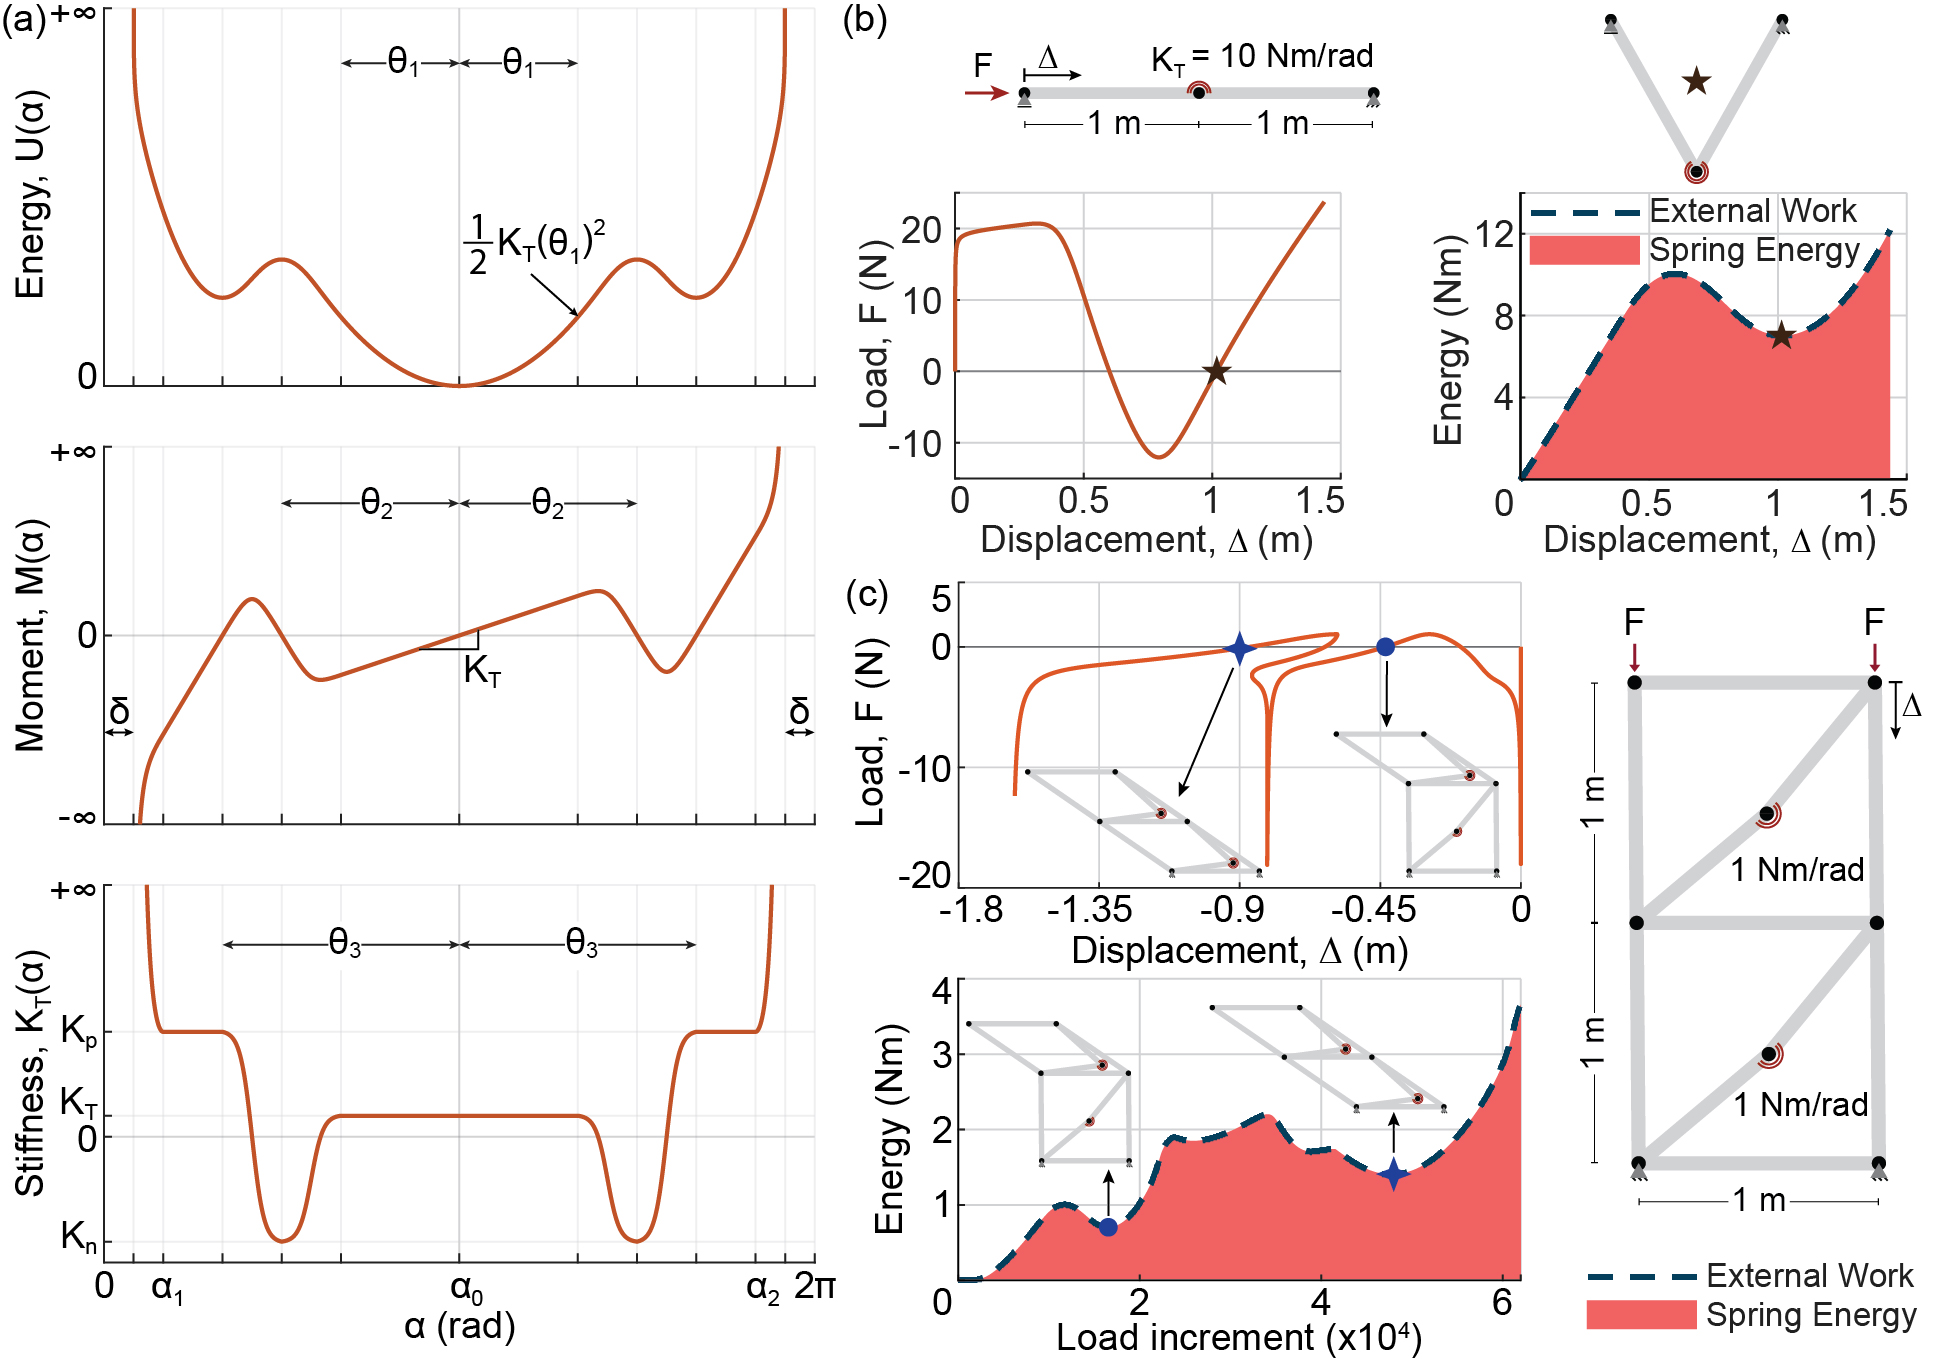
\includegraphics[width=\textwidth]{01-figures/04-05-bistable-hinge-modeling.jpg}
  \caption{Bistable torsional hinge: (a) Schematic representation of the strain energy (top), restoring moment (middle), and tangent stiffness (bottom) curves for a bistable torsional hinge with respect to the relative angle of the hinge; (b) Load vs. Displacement (left) and System energy vs. Displacement (right) curves for the buckling of colinear bars in compression fitted with a bistable torsional hinge.}\label{fig-bistable-hinge}
\end{figure}
\subsection{Computational Formulation of Bistable Torsional Spring for Matrix Structural Analysis}\label{04-subsec-bistable-equations}
Within the central angular interval \(\alpha_1<\alpha<\alpha_2\), the
bistable torsional spring is described using the relative rotation
\begin{equation}
\theta=\alpha-\alpha_0,
\label{eq:theta}
\end{equation}
where \(\alpha_0\) is the stress-free reference angle. The response outside
\(\alpha_1<\alpha<\alpha_2\) is modeled using the enhanced spring law described
in the preceding section.

The spring is defined by an initial stiffness \(K_T\), a negative stiffness
\(k_{\mathrm{neg}}\), and a post-transition positive stiffness
\(k_{\mathrm{pos}}\). The transition rotations satisfy
\begin{equation}
0<\theta_1<\theta_2<\theta_3.
\label{eq:transition-widths}
\end{equation}
The smooth transition function is
\begin{equation}
q(s)=
\frac{
\tanh\!\left[\beta\left(s-\frac{1}{2}\right)\right]
+\tanh\!\left(\frac{\beta}{2}\right)
}{
2\tanh\!\left(\frac{\beta}{2}\right)
},
\qquad 0\le s\le 1,
\label{eq:q}
\end{equation}
where \(s\) is the local normalized coordinate within a transition interval and
\(\beta\) controls the sharpness of the transition. The function satisfies
\(q(0)=0\) and \(q(1)=1\), so it smoothly interpolates between two prescribed
stiffness values over one transition interval. Larger values of \(\beta\)
produce a sharper transition, while smaller values produce a more gradual
transition. Its first and second primitives are denoted by
\begin{equation}
Q(s)=\int_0^s q(u)\,du,
\qquad
\mathcal{Q}(s)=\int_0^s Q(v)\,dv.
\label{eq:q-primitives}
\end{equation}

The moment levels at the positive transition rotations are
\begin{align}
M_1 &= K_T\theta_1, \label{eq:M1}\\
M_2 &=
M_1
+(\theta_2-\theta_1)
\left[
K_T+\left(k_{\mathrm{neg}}-K_T\right)Q(1)
\right],
\label{eq:M2}\\
M_3 &=
M_2
+(\theta_3-\theta_2)
\left[
k_{\mathrm{neg}}
+\left(k_{\mathrm{pos}}-k_{\mathrm{neg}}\right)Q(1)
\right].
\label{eq:M3}
\end{align}
The corresponding energy levels are
\begin{align}
U_1 &=
\frac{1}{2}K_T\theta_1^2, \label{eq:U1}\\
U_2 &=
U_1+(\theta_2-\theta_1)M_1
+(\theta_2-\theta_1)^2
\left[
\frac{1}{2}K_T
+\left(k_{\mathrm{neg}}-K_T\right)\mathcal{Q}(1)
\right],
\label{eq:U2}\\
U_3 &=
U_2+(\theta_3-\theta_2)M_2
+(\theta_3-\theta_2)^2
\left[
\frac{1}{2}k_{\mathrm{neg}}
+\left(k_{\mathrm{pos}}-k_{\mathrm{neg}}\right)\mathcal{Q}(1)
\right].
\label{eq:U3}
\end{align}

The tangent stiffness in the central region is
\begin{equation}
k_T(\theta)=
\begin{cases}
k_{\mathrm{pos}},
& \theta<-\theta_3,\\[4pt]
k_{\mathrm{neg}}
+\left(k_{\mathrm{pos}}-k_{\mathrm{neg}}\right)
q\!\left(\dfrac{-\theta-\theta_2}{\theta_3-\theta_2}\right),
& -\theta_3\le\theta<-\theta_2,\\[12pt]
K_T+\left(k_{\mathrm{neg}}-K_T\right)
q\!\left(\dfrac{-\theta-\theta_1}{\theta_2-\theta_1}\right),
& -\theta_2\le\theta<-\theta_1,\\[12pt]
K_T,
& -\theta_1\le\theta\le\theta_1,\\[4pt]
K_T+\left(k_{\mathrm{neg}}-K_T\right)
q\!\left(\dfrac{\theta-\theta_1}{\theta_2-\theta_1}\right),
& \theta_1<\theta\le\theta_2,\\[12pt]
k_{\mathrm{neg}}
+\left(k_{\mathrm{pos}}-k_{\mathrm{neg}}\right)
q\!\left(\dfrac{\theta-\theta_2}{\theta_3-\theta_2}\right),
& \theta_2<\theta\le\theta_3,\\[12pt]
k_{\mathrm{pos}},
& \theta>\theta_3.
\end{cases}
\label{eq:stiffness}
\end{equation}

The restoring moment is obtained by integrating the stiffness with respect to
\(\theta\) and enforcing \(M(0)=0\):
\begin{equation}
M(\theta)=
\begin{cases}
-M_3+k_{\mathrm{pos}}(\theta+\theta_3),
& \theta<-\theta_3,\\[6pt]
-M_2-(\theta_3-\theta_2)\left[
k_{\mathrm{neg}}s_+^-
+\left(k_{\mathrm{pos}}-k_{\mathrm{neg}}\right)Q(s_+^-)
\right],
& -\theta_3\le\theta<-\theta_2,\\[10pt]
-M_1-(\theta_2-\theta_1)\left[
K_Ts_-^-
+\left(k_{\mathrm{neg}}-K_T\right)Q(s_-^-)
\right],
& -\theta_2\le\theta<-\theta_1,\\[10pt]
K_T\theta,
& -\theta_1\le\theta\le\theta_1,\\[6pt]
M_1+(\theta_2-\theta_1)\left[
K_Ts_-^+
+\left(k_{\mathrm{neg}}-K_T\right)Q(s_-^+)
\right],
& \theta_1<\theta\le\theta_2,\\[10pt]
M_2+(\theta_3-\theta_2)\left[
k_{\mathrm{neg}}s_+^+
+\left(k_{\mathrm{pos}}-k_{\mathrm{neg}}\right)Q(s_+^+)
\right],
& \theta_2<\theta\le\theta_3,\\[10pt]
M_3+k_{\mathrm{pos}}(\theta-\theta_3),
& \theta>\theta_3,
\end{cases}
\label{eq:moment}
\end{equation}
where the scaled transition coordinates are
\begin{equation}
s_-^-=\frac{-\theta-\theta_1}{\theta_2-\theta_1},
\qquad
s_+^-=\frac{-\theta-\theta_2}{\theta_3-\theta_2},
\qquad
s_-^+=\frac{\theta-\theta_1}{\theta_2-\theta_1},
\qquad
s_+^+=\frac{\theta-\theta_2}{\theta_3-\theta_2}.
\label{eq:s-coordinates}
\end{equation}

The strain energy is defined by \(U(0)=0\) and
\(M=dU/d\theta\). In the central region,
\begin{equation}
U(\theta)=
\begin{cases}
U_3-M_3(\theta+\theta_3)
+\dfrac{1}{2}k_{\mathrm{pos}}(\theta+\theta_3)^2,
& \theta<-\theta_3,\\[10pt]
U_2+(\theta_3-\theta_2)M_2s_+^-
+(\theta_3-\theta_2)^2\left[
\dfrac{1}{2}k_{\mathrm{neg}}(s_+^-)^2
+\left(k_{\mathrm{pos}}-k_{\mathrm{neg}}\right)\mathcal{Q}(s_+^-)
\right],
& -\theta_3\le\theta<-\theta_2,\\[14pt]
U_1+(\theta_2-\theta_1)M_1s_-^-
+(\theta_2-\theta_1)^2\left[
\dfrac{1}{2}K_T(s_-^-)^2
+\left(k_{\mathrm{neg}}-K_T\right)\mathcal{Q}(s_-^-)
\right],
& -\theta_2\le\theta<-\theta_1,\\[14pt]
\dfrac{1}{2}K_T\theta^2,
& -\theta_1\le\theta\le\theta_1,\\[10pt]
U_1+(\theta_2-\theta_1)M_1s_-^+
+(\theta_2-\theta_1)^2\left[
\dfrac{1}{2}K_T(s_-^+)^2
+\left(k_{\mathrm{neg}}-K_T\right)\mathcal{Q}(s_-^+)
\right],
& \theta_1<\theta\le\theta_2,\\[14pt]
U_2+(\theta_3-\theta_2)M_2s_+^+
+(\theta_3-\theta_2)^2\left[
\dfrac{1}{2}k_{\mathrm{neg}}(s_+^+)^2
+\left(k_{\mathrm{pos}}-k_{\mathrm{neg}}\right)\mathcal{Q}(s_+^+)
\right],
& \theta_2<\theta\le\theta_3,\\[14pt]
U_3+M_3(\theta-\theta_3)
+\dfrac{1}{2}k_{\mathrm{pos}}(\theta-\theta_3)^2,
& \theta>\theta_3.
\end{cases}
\label{eq:energy}
\end{equation}
Equations~\eqref{eq:stiffness}--\eqref{eq:energy} define the bistable spring
law used for \(\alpha_1<\alpha<\alpha_2\).

\subsection{Structural Response of Reconfigurable Trusses with Bistable Torsional Hinges}\label{04-subsec-bistable-examples}
This subsection presents two example structures fitted with bistable torsional hinges. The examples demonstrate how the proposed formulation can represent highly nonlinear hinge response within the structural analysis of reconfigurable trusses. A physical prototype of this idealized bistable torsional spring has not yet been developed. Therefore, the examples are intended as computational demonstrations of the modeling capability. They show how bistable hinge laws can be used to study snap-through, post-transition stiffening, and transitions between multiple stable states.

Both examples use the bistable torsional spring law described in the previous subsection. The bistable hinge's transition points are set to \(\theta_1=60^\circ{}\), \(\theta_2=90^\circ{}\), and \(\theta_3=120^\circ{}\). The negative stiffness value is defined using \(K_n=-5K_T\), and the post-transition positive stiffness branch is defined using \(K_p=5K_T\). The admissible hinge rotation is bounded using the same asymptotic stiffening strategy introduced in the enhanced spring law from Section~\ref{04-subsec-enhanced-spring}. The corresponding angular-limit parameters are \(\delta=15^\circ{}\), \(\alpha_1=30^\circ{}\), and \(\alpha_2=330^\circ{}\). These limits restrict the deformation of the hinge in the inverval (15\(^\circ\), 345\(^\circ\)).

The first example consists of two collinear bars connected by a bistable torsional hinge and loaded in compression, as shown in Fig.~\ref{fig-bistable-hinge},(b). The left end is modeled as a roller support, the right end is modeled as a pinned support, and the bistable torsional spring is placed at the connection between the two bars. Each bar has a length of 1~m, elastic modulus \(E=3\times10^9~\text{N/m}^2\), and cross-sectional area \(A=0.5~\text{m}^2\). The baseline torsional spring stiffness is \(K_T=10~\text{Nm/rad}\).

As the imposed displacement (\Delta) increases in the positive (x)-direction, the applied load initially rises to approximately 20~N. An elastic instability then develops at the central hinge, and the structure snaps away from the initial collinear configuration. During this transition, the load required to continue deformation decreases and becomes negative. This response indicates that the structure tends to move toward the next stable state once the instability is triggered. The second stable state occurs near \(\Delta=1~\text{m}\). This configuration is marked with a star on the load-displacement curve, the energy plot, and the corresponding deformed configuration in Fig.~\ref{fig-bistable-hinge},(b). At this state, the spring-energy curve exhibits a local minimum, which is consistent with a stable equilibrium configuration. Further displacement beyond this point drives the hinge into the post-transition positive-stiffness regime. As a result, the applied load increases again.

The second example considers a reconfigurable truss with two independent kinematic degrees of freedom. The structure, shown in Fig.~\ref{fig-bistable-hinge}\,(c), is the same stacked square-linkage truss introduced in Fig.~\ref{fig-deployment-path}\,(a), but each spring is now modeled as a bistable torsional hinge. In this example, the baseline torsional stiffness is set to \(K_T=1~\text{Nm/rad}\) for each hinge.

As vertical compression is applied to the structure, the load magnitude first increases rapidly with little global displacement. An elastic instability then develops in the upper square-linkage unit. The upper unit snaps into its next stable state, producing a sharp drop in the applied load. This first stable state is marked with a blue circle in Fig.~\ref{fig-bistable-hinge},(c). After this transition, the upper hinge enters its post-transition positive-stiffness branch, and additional deformation is redirected to the lower unit.

With continued compression, the load rises again until a second instability develops in the lower square-linkage unit. The lower unit then snaps into its next stable state. This second stable state is marked with a blue star in Fig.~\ref{fig-bistable-hinge},(c). The blue circle and blue star are also identified on the spring-energy plot, where they correspond to local minima associated with stable equilibrium configurations.

These examples show that bistable torsional hinges can introduce multiple stable configurations into reconfigurable trusses. In the single-hinge example, the structure transitions between two stable states. In the stacked truss, the two independent kinematic degrees of freedom produce a sequence of stable-state transitions. The analysis therefore demonstrates how nonlinear hinge laws can be used to program the deployment path and stable configurations of reconfigurable truss systems.

\section{Discussion}\label{04-sec-discussion}

\section{Concluding Remarks}\label{04-sec-conclusion}
\chapter{Rapidly Deployable Hulls and On-demand Tunable Hydrodynamics with Shape Morphing Curved Crease Origami}\label{chapter-05}
Traditional hull fabrication relies on labour- and time-intensive methods to generate smooth, curved surfaces. These conventional methods often lead to hull surface topologies that are static in design with hydrodynamics aimed at handling a broad range of sea conditions but not optimized for any specific scenario. In this chapter, we introduce a method of rapidly fabricating planing hulls using the principles of curved-crease origami. Starting from a flat-folded state, the curved-crease origami hulls can be deployed to match traditional planing hull shapes like the VPS (deep-V, Planing hull with Straight face) and the GPPH (General Purpose Planing Hull). By extension of the ability to conform to a desired shape, we show that the curved-crease origami hulls can emulate desired hydrodynamic characteristics in still as well as wavy water conditions. Furthermore, we demonstrate the shape-morphing ability of curved-crease origami hulls, enabling them to switch between low and high deadrise configurations. This ability allows for on-demand tuning of the hull hydrodynamic performance. We present proof-of-concept origami hulls to demonstrate the practical feasibility of our method. Hulls fabricated using the curved-crease origami principles can adapt to different sea states, and their flat foldability and deployment facilitate easy transport and deployment for rapid response naval operations such as rescue missions and the launch of crewless aquatic vehicles. This work has been published as \href{https://doi.org/10.1016/j.jfluidstructs.2024.104176}{\textbf{Patil, H. Y.}, Maki, K. J., \& Filipov, E. T. (2024). Rapidly deployable hulls and on-demand tunable hydrodynamics with shape morphing curved crease origami. Journal of Fluids and Structures, 130, 104176}~\cite{patil2024ccohulls}.

\section{Introduction}\label{05-sec-origami-hull-intro}
Advanced boat-building and sailing technologies have existed since 6000 BCE~\cite{carter_boat_2006}. Despite the impressive technological strides in naval engineering over centuries, hull fabrication continues to be an enduring and intricate task. Hull fabrication relies on labor-intensive methods that involve connecting numerous flat sheets through bolting, riveting, or welding to form smooth, curved surfaces~\cite{paoli_fabrication_2012}. Achieving the necessary smooth curved surfaces also requires complex casting, milling, and molding procedures. Another challenge is that a significant portion of hull fabrication occurs in landlocked regions, necessitating the transportation of ship parts to coastal docks for assembly~\cite{bruce_ship_2021}. This transportation further extends the construction timeline and associated costs. These current hull fabrication techniques lead to designs with static surface topologies, resulting in hydrodynamics that are a compromise to accommodate a broad spectrum of sea conditions. Consequently, these hulls are not optimized for specific conditions, often leading to inefficient power consumption, poor maneuverability, and reduced passenger comfort and safety. For instance, crew members experience musculoskeletal pain and mental fatigue due to repeated exposure to vertical accelerations caused by the porpoising motion of vessels~\cite{bjorn_crew_2017}. These multifaceted challenges underscore the need to adopt innovative approaches in the shipbuilding industry, focusing on more versatile fabrication processes and improved adaptability in hull performance.

Origami, the age-old art of paper folding, presents a promising extension to the existing fabrication techniques used by the shipbuilding industry. In recent years, origami has transcended its traditional boundaries and found remarkable applications in engineering structures~\cite{meloni_engineering_2021}. One key characteristic of origami-inspired structures is their ability to transform flat sheets into complex, three-dimensional structures. This geometrically transformative process dynamically changes the properties of structures and the surrounding fluid media to meet multiple design objectives by varying the extent of folding, as shown by~\cite{chen_drag_2023} and~\cite{origami_flexiball_2023}. Origami-inspired designs embody several advantageous characteristics, each with unique applications. For instance, structures designed using origami principles can be rapidly deployed from compact configurations and easily reconfigured for various functions~\cite{zirbel_hanaflex_2015}. This reconfigurability has potential applications, such as creating stents for minimally invasive surgeries in biomedical engineering~\cite{kuribayashi_stent_2006} and improving the storage and deployment of satellites and solar arrays in space structures~\cite{bowen_starshade_2016}. Origami principles are also scale-independent~\cite{dudte_scale_2016}, making them applicable to structures ranging from deployable stadium canopies to micro-scale sensors. Additionally, the active folding capability enables these structures to change form on demand, increasing their adaptability to various loads and conditions \textemdash{} a strategy often employed by biological organisms to survive in strong winds or water currents~\cite{harder_reconfiguration_2004}. Thus, incorporating origami principles into ship hull design offers benefits such as flat foldability, efficient storage and transport, and rapid deployment.

While traditional origami surfaces such as Miura-ori~\cite{k_science_2008} are characterized by rough and angular profiles, curved-creasing \textemdash{} a subset of origami, provides a groundbreaking approach to fabricating hull-type structures in naval engineering. Research by~\cite{erik_demaine_curved_2011} demonstrates that folding a sheet of material along arbitrary non-intersecting curved creases enables rapid and easy fabrication of smooth curved surfaces. Curved-crease origami preserves the inherent merits of conventional origami techniques while offering numerous benefits suited for hull fabrication. For instance, curved creasing grants precise control over surface topologies by tuning the crease geometry and extent of actuation. Furthermore, it enables the fabrication of complex 3-D shapes that embody benefits such as reduced joint complexity, increased global stiffness, and improved resistance to buckling~\cite{woodruff_curved_2021}.

Motivated by the potential of curved-crease origami principles, this chapter presents an approach for fabricating planing hulls. Planing hulls commonly feature a V-shaped bottom and a transom stern design, which generates hydrodynamic lift to support the hull weight and enable high-speed travel. As a result, these hulls are widely used for applications such as Coast Guard boats, rescue vessels, and ocean racers~\cite{savitsky_planing_1985}. \cite{tavakoli_review_2024} provides a detailed review of the topology and hydrodynamics of planing hulls. The inherent geometry of planing hulls (see Section~\ref{05-sec-geometry-curved-folding}) makes them an ideal candidate for incorporating curved-crease origami-based fabrication techniques. Thus, as a first step towards curved-crease origami-based hulls, we limit the scope of our exploration to idealized planing hulls. While we agree that extending origami principles to general hull forms poses several challenges at this stage, it still holds significant potential for curved surface fabrication and will be explored separately in the future.

By leveraging the principles of origami, we demonstrate the capability to reproduce a predetermined target planing hull shape with precision. This capability enables the emulation of a desired hydrodynamic behavior and embodies the fabrication efficiency inherent to curved crease origami. Furthermore, through the strategic utilization of active folding in curved-crease origami hulls, we illustrate their ability to undergo a characteristic shape change in real-time. This shape morphing behavior enables on-demand tunability of hydrodynamic properties and renders them applicable across a wide variety of sea conditions. Hulls fabricated using the proposed methods can adapt to any sea state, and their flat foldability and rapid deployment will facilitate easy transport and deployment for naval operations such as covert rescue missions and the launch of crewless decoy marine vehicles. These vehicles will also improve sea-keeping performance, power efficiency, maneuverability, and passenger comfort, making them suitable for civilian recreational use.

The remainder of the chapter is organized as follows. Section~\ref{05-sec-geometry-curved-folding} reviews standard planing hull geometries and curved folding procedures. The subsections discuss the planing behavior and typical geometric features of a planing hull, the development of a curved-origami crease pattern for the planing hull, an overview of the numerical model for curved-origami folding, and geometric parameter optimization to match curved-origami hulls to their target shape. Next, Section~\ref{05-sec-hydrodynamic-analysis} explores the hydrodynamic analyses and performance evaluation of curved origami planing hulls against target hull shapes. The core findings of this chapter, including the on-demand shape morphing capabilities of curved-origami hulls and tunable hydrodynamic characteristics for a wide range of sea conditions, are presented in Section~\ref{05-sec-tunable-hydrodynamics}. A discussion on the scalability of origami hulls with an emphasis on curvature analysis for various construction materials is presented in Section~\ref{05-sec-physical-implementation}. Finally, concluding remarks summarizing the key contributions are included in Section~\ref{05-sec-hull-conclusion}.

\section{Geometry and Curved Folding}\label{05-sec-geometry-curved-folding}    

\subsection{Planing Hull Geometry}\label{05-subsec-planing-geometry}
In a state of rest, buoyant forces are responsible for bearing the weight of a floating hull. Buoyancy is also crucial at lower speed since the hull stays afloat by displacing a volume of water. However, as the speed increases, hydrodynamic lift becomes dominant over the buoyant force and supports the weight of the hull. This hydrodynamic lift allows a planing hull to rise and glide on the water surface.

A typical planing hull has distinct geometric features that enable it to generate hydrodynamic lift. These geometric features of a planing hull (some illustrated in Fig.~\ref{fig-planing-geometry}\,(a)) can be defined as follows: \mbox{(\textit{i}\hspace{.5pt})} \textit{Bow}: the foremost part of the hull; \mbox{(\textit{ii}\hspace{.5pt})} \textit{Chine}: line along which a sharp change in the angle of cross-section occurs; \mbox{(\textit{iii}\hspace{.5pt})} \textit{Deadrise}: the angle between the bottom of the hull and horizontal surface; \mbox{(\textit{iv}\hspace{.5pt})} \textit{Draft}: the distance between the waterline and the deepest part of the boat in steady state; \mbox{(\textit{v}\hspace{.5pt})} \textit{Hull Bottom}: bottom surface of the hull (also called the planing surface); \mbox{(\textit{vi}\hspace{.5pt})} \textit{Keel}: bottom-most longitudinal structural element of a hull; \mbox{(\textit{vii}\hspace{.5pt})} \textit{Sheer line}: the uppermost edge of the hull; \mbox{(\textit{viii}\hspace{.5pt})} \textit{Stern}: the aftmost part of the hull; \mbox{(\textit{ix}\hspace{.5pt})} \textit{Transom}: the flat board extending from the keel to the deck at the stern; \mbox{(\textit{x}\hspace{.5pt})} \textit{Trim}: the angle between the horizontal surface and the line connecting the forward and the aft draft; and \mbox{(\textit{xi}\hspace{.5pt})} \textit{Waterline}: the level water reaches on the hull's side. In some cases, the hull has a parallel section and can be divided into two parts longitudinally, namely the prismatic and non-prismatic sections. The prismatic section often forms the middle to aft half of the hull where the keel and chine lines are parallel. On the other hand, the non-prismatic section forms the front portion of the hull where the keel and chine lines are no longer parallel.

It is important to note that the planing hulls discussed in this chapter are hard-chined vessels, which means that the hull exhibits a distinct change of angle along the chine, where the bottom surface meets the sides of the boat. Additionally, these planing hulls feature a typical V-shaped bow with straight surfaces instead of an axe, bulbous, parabolic, or flared bow.

\begin{figure}[!htbp]
  \centering
  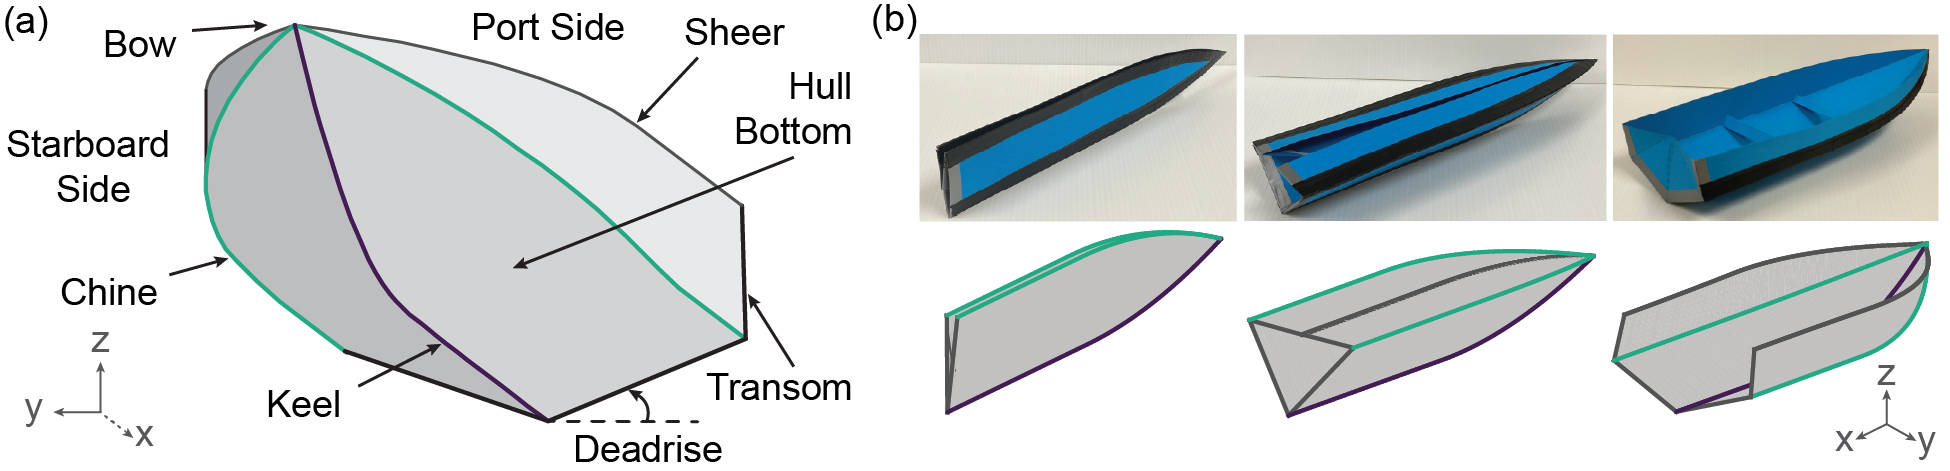
\includegraphics[width=\textwidth]{01-figures/05-01-geometry-and-hull-folding.jpg}
  \caption{(a) Geometric features of a typical planing hull: specifically a deep V-shape, Planing hull with a Straight planing surface (VPS); (b) Sequential deployment of curved-crease origami hull designed to match the shape of a VPS hull: paper model (top) compared with Bar and Hinge simulation (bottom). A transom is not included in the simulation.}\label{fig-planing-geometry}
\end{figure}

The curved-crease origami-inspired planing hulls offer a method to change some of the aforementioned geometric features that directly affect the hull's planing ability, stability, ride comfort, maneuverability, and power efficiency. Throughout its deployment, the curved crease origami hulls can vary the deadrise, hull length, topology of the curved planing surface, and beam length. The deployment process from a flat-folded to a deployed-hull state is shown in Fig.~\ref{fig-planing-geometry}\,(b) for both a 20-inch long paper prototype and for a corresponding Bar and Hinge simulation (discussed in the following section). The planing hull design, obtained using the bar and hinge model, is presented here without the transom to reveal distinctive features of the hull, including the chine, keel, and profile of the planing surface. However, the transom can be incorporated into the model, akin to the paper prototype shown in Fig.~\ref{fig-planing-geometry}\,(b).

\subsection{Crease Geometry and Bar and Hinge Model for Curved Folding}\label{05-subsec-crease-bnh}
A curved crease pattern presented in Fig.~\ref{fig-crease-bnh}\,(a) is developed to match the VPS hull designed by~\cite{kim_design_2013}. VPS stands for deep V-shape, Planing hull with a Straight planing surface, and resembles the shape illustrated in Fig.~\ref{fig-planing-geometry}\,(a). This crease pattern unfolds into a 3D shape with all the geometric features of a typical planing hull. The geometric parameters used to define this crease pattern are: \mbox{(\textit{i}\hspace{.5pt})} width of the hull's bottom surface between the chine and the keel, \(H\); \mbox{(\textit{ii}\hspace{.5pt})} height of the tip, \(h_{\textrm{tip}}\); \mbox{(\textit{iii}\hspace{.5pt})} overall length of the crease pattern, \(L_{OA}\); \mbox{(\textit{iv}\hspace{.5pt})} length of the prismatic part of the chine, \(L_{P}^{c}\); \mbox{(\textit{v}\hspace{.5pt})} length of the non-prismatic part of the chine, \(L_{N}^{c}\); \mbox{(\textit{vi}\hspace{.5pt})} length of the prismatic part of the keel, \(L_{P}^{k}\); and \mbox{(\textit{vii}\hspace{.5pt})} length of the non-prismatic part of the keel, \(L_{N}^{k}\). The curved portions (non-prismatic section) of the chine and the keel curves are parabolic and denoted by \(y_c\) in Eq.~\ref{eq-chine-curve} and \(y_k\) in Eq.~\ref{eq-keel-curve}, respectively. For a given overall length of the crease pattern, the length of the non-prismatic section for the chine and keel curves are denoted by \(L_N^c\) in Eq.~\ref{eq-np-chine} and \(L_N^k\) in Eq.~\ref{eq-np-keel}, respectively. These quantities can be computed as:
\begin{flalign}
  \quad L_{N}^{c} & = L_{OA} - L_{P}^{c}~,&\label{eq-np-chine}\\
  \quad L_{N}^{k} & = L_{OA} - L_{P}^{k}~,&\label{eq-np-keel}\\
  \quad y_{k} & = \left[\frac{h_{\textrm{tip}}}{{L_{N}^{k}}^2}\right]\times\left(x-L_{P}^{k}\right)^2~,&\label{eq-keel-curve}\\
  \quad y_{c} & = \left[\frac{h_{\textrm{tip}}-H}{{L_{N}^{c}}^2}\right]\times\left(x-L_{P}^{c}\right)^2 + H~.&\label{eq-chine-curve}
\end{flalign}

\begin{figure}[!htbp]
  \centering
  \includegraphics[width=\textwidth]{01-figures/05-02-crease-pattern-and-bar-hinge.jpg}
  \caption{(a) Geometric parameters defining the curved crease pattern for a planing hull shape; (b) Folded curved-crease origami hull shape viewed from starboard side; (c) Flat, intermediate, and fully folded (clockwise from top) curved-crease origami hull shape viewed from the Transom (also known as Stern) side; and (d) Decomposition of the Bar and Hinge model into its components: in-plane bars, bending hinges, and folding hinges.}\label{fig-crease-bnh}
\end{figure}

The curved folding simulation of the origami crease pattern into a planing hull shape is accomplished through the Bar and Hinge model developed by~\cite{woodruff_bar_2020}. This model offers a simplified numerical approach that effectively simulates the fundamental behaviours of curved origami folding by employing three distinct elements, as illustrated in Fig.~\ref{fig-crease-bnh}. These elements can be described as follows: \mbox{(\textit{i}\hspace{.5pt})} three-dimensional truss elements, or bars, that capture in-plane stretching and shearing of the sheet; \mbox{(\textit{ii}\hspace{.5pt})} rotational springs, or hinges, that capture the out-of-plane bending of the sheet by consolidating bending into discrete rotations along the bar lengths; and \mbox{(\textit{iii}\hspace{.5pt})} another set of hinges that capture the rotations at the creases or fold lines.

The crease pattern is meshed using a combination of the three elements, where the stiffness of each element is determined based on material properties, sheet thickness, and mesh size. Despite the inherent geometric nonlinearity involved in the folding process, the model achieves convergence within a short time frame (less than 10 seconds). This rapid convergence is due to the relatively low number of elements in the Bar and Hinge model compared to finite element methods. Consequently, this rapid simulation enables efficient analysis of curved origami structures, facilitating subsequent shape-matching and optimization processes.

\subsection{Shape Matching and Optimization}\label{05-subsec-shape-matching}
The geometric design parameters presented in Fig.~\ref{fig-crease-bnh}\,(a) can be varied and optimized such that the curved crease origami (CCO) hull shape will match the desired target shape. The matching of CCO hull with target hull shapes is significant for two reasons. Firstly, it enables the reproduction of specific hydrodynamic characteristics by replicating the target shape. Secondly, it facilitates the integration of origami-based design principles in conventional hull design, thereby unlocking the potential to design on-demand shape morphing hulls with tunable hydrodynamics. This section will explore two design variations of the CCO hulls, CCO\(^\textrm{VPS}\) and CCO\(^\textrm{GPPH}\), and compare their shapes with those of the VPS and the General Purpose Planing Hull (GPPH) shapes, respectively.

\begin{figure}[!htbp]
  \centering
  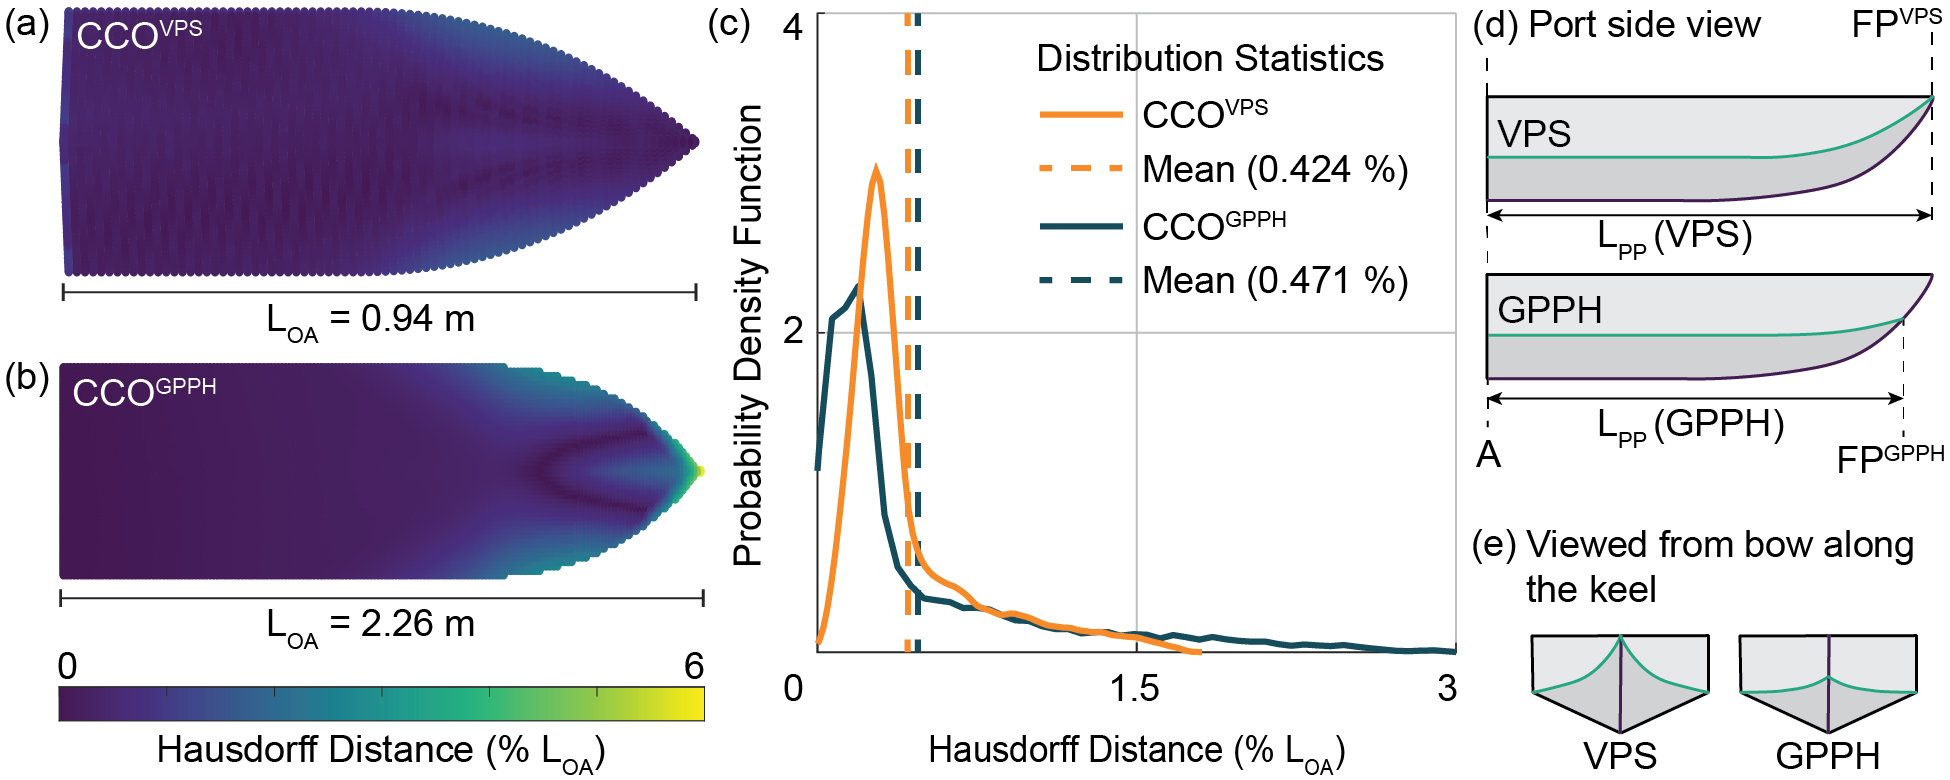
\includegraphics[width=\textwidth]{01-figures/05-03-hausdorff-shape-matching-optimization.jpg}
  \caption{Color heat map showing the Hausdorff distance as a percentage of the overall hull length (\(L_{OA}\)) for the planing surface of two different CCO hull designs compared with: (a) 0.94 m long VPS hull and (b) 2.26 m long GPPH, respectively; (c) Hausdorff distance distribution statistics for CCO hull designs' planing surface compared with corresponding VPS and GPPH designs; (d) Port side view depicting the location of forward perpendicular (FP), aft perpendicular (AP) and the length between the two perpendiculars (\(L_{PP}\)); and (e) Bow view when looked along the keel of the VPS and GPPH showing the difference in the chine and keel configuration.}\label{fig-shape-matching}
\end{figure}

The quantification of dissimilarity between a CCO hull shape and a target shape is performed using a parameter called the Hausdorff distance, \(d_H\). By definition, the Hausdorff distance represents the maximum distance between any point in one set and the closest point in the other set in three-dimensional space, indicating the largest discrepancy between the two point sets. Hence, smaller Hausdorff distances between two sets (two shapes in this case) indicate a closer match. To ensure consistency in comparing the two different design variants of the CCO hulls with their target shapes, we will represent the Hausdorff distance as the percentage of the overall length, \(L_{OA}\) of the hull's planing surface. We specifically emphasize comparing the planing surface because its interaction with water is the predominant factor that influences the hydrodynamic behavior of the hull.

The planing surfaces of CCO\(^\textrm{VPS}\) and VPS hulls are populated with approximately 5000 points, and the Hausdorff distance for each point on the CCO\(^\textrm{VPS}\) hull is computed with respect to the VPS hull (Fig.~\ref{fig-shape-matching}\,(a)). As the folded shape of the CCO\(^\textrm{VPS}\) hull is influenced by the geometric parameters of the curved-crease pattern, a simple optimization problem is formulated to find optimal values that minimize the Hausdorff distance between the two hulls. The objective of this problem is to minimize the mean Hausdorff distance between the two hulls, considering the following design variables: \mbox{(\textit{i}\hspace{.5pt})} overall length of crease pattern (\(L_{OA}\)), \mbox{(\textit{ii}\hspace{.5pt})} width of the planing panel (\(H\)), \mbox{(\textit{iii}\hspace{.5pt})} tip height (\(h_\textrm{tip}\)), \mbox{(\textit{iv}\hspace{.5pt})} length of the prismatic part of chine (\(L_P^c\)), \mbox{(\textit{v}\hspace{.5pt})} length of the prismatic part of the keel (\(L_P^k\)), and  \mbox{(\textit{vi}\hspace{.5pt})} deadrise of the hull. The optimizer successfully achieves a mean Hausdorff distance of 0.424\% and a maximum Hausdorff distance of under 2\% of the overall length of the hull, indicating an excellent match between the two shapes. This method enables on-demand replication of hull shapes using curved-crease origami principles for innovative hull design and hydrodynamic optimization.

A similar shape-matching procedure is performed for the CCO\(^\textrm{GPPH}\) and the GPPH hulls with approximately 7500 points. In this case, the mean Hausdorff distance is observed to be 0.471\%, and the maximum Hausdorff distance is under 6\% of the overall GPPH length. The larger Hausdorff distances compared to the previous case, particularly towards the bow of the hull (see Fig.~\ref{fig-shape-matching}\,(b)), can be explained by the difference in the keel extension of the hull designs. As illustrated in Fig.~\ref{fig-shape-matching}\,(d) and (e), the keel line of the GPPH extends beyond the chine. Meanwhile, the chine and keel lines of the VPS and both CCO hull designs terminate at the same point on the hull's bow. This difference in keel extension leads to a dissimilar bow shape in the GPPH design compared to the VPS and both CCO hull designs, thus explaining the higher Hausdorff distances.

Despite the minor dissimilarities observed near the bow of the hull in the cases of the VPS and GPPH, the CCO hulls achieve a close match over the prismatic section of the planing surface. The mean Hausdorff distance for the prismatic section of VPS and GPPH equivalent CCO hulls is observed to be 0.258\% and 0.281\% of the overall length, respectively.  Furthermore, the distribution of Hausdorff distances shown in Fig.~\ref{fig-shape-matching}\,(c) indicates that the mean Hausdorff distance is less than 0.5\% of the overall length for most parts of the planing surface that would interact with water. This similarity in shape and deadrise ensures that the CCO hull can potentially exhibit hydrodynamic characteristics comparable to those of the conventional VPS and GPPH hull designs. Detailed findings related to the hydrodynamic properties and the comparison between the CCO hulls, VPS, and GPPH are presented and discussed in the subsequent sections.

\section{Hydrodynamic Performance Evaluation of Curved-crease Origami Hulls}\label{05-sec-hydrodynamic-analysis}
The ability of curved-crease origami (CCO) hulls to align congruently with target hull shapes motivates a comparative investigation to evaluate whether their hydrodynamic characteristics also match those of the conventional hulls. This section compares the hydrodynamic performance of the two distinct CCO hull variants, CCO\(^\textrm{VPS}\) and CCO\(^\textrm{GPPH}\) as introduced in Section~\ref{05-subsec-shape-matching}, with their corresponding target hull forms, namely the VPS and the GPPH. The hydrodynamic evaluation for all four hull geometries is facilitated by the Powersea tool and encompasses the simulation of hull motion in both still and wavy water (head sea) conditions. Powersea's underlying theory, assumptions and limitations can be found in Appendix~\ref{03-appendix-powersea}. The geometric and physical characteristics of the hulls passed as input to Powersea can be found in Table~\ref{tab-cco-hull-geom}.
\begin{table}[h!]
  \caption{Geometric and physical characteristics of the hulls for hydrodynamic simulations}
  \vspace{-1.5em}
  \begin{center}
	\begin{tabularx}{\textwidth}{ >{\raggedright\arraybackslash}X >{\centering\arraybackslash}m{0.4in} >{\centering\arraybackslash}m{0.4in} >{\centering\arraybackslash}m{0.6in} >{\centering\arraybackslash}m{0.6in} >{\centering\arraybackslash}m{0.6in} >{\centering\arraybackslash}m{0.7in} >{\centering\arraybackslash}m{0.5in} }
  	\hline
  	\multirow{2}{3.5in}{\textbf{Hull geometry}} & \textbf{L$_{OA}$} & \textbf{L$_{PP}$} & \textbf{LCG } & \textbf{VCG} & \textbf{K$_{yy}$} & \textbf{Weight} & \textbf{B}\\
  	& (m) & (m) & (\% L$_{OA}$) & (m) & (\% L$_{OA}$) & (N) & (m)\\
  	\hline
    \noalign{\vskip 3pt}
  	CCO\(^\textrm{VPS}\) & 0.94 & 0.92 & 62 & 0.056 & 25 & 65 & 0.312\\  
  	VPS & 0.94 & 0.92 & 62 & 0.056 & 25 & 65 & 0.308\\
  	CCO\(^\textrm{GPPH}\) & 2.26 & 2.26 & 62 & 0.097 & 25 & 995.51 & 0.583\\
  	GPPH & 2.26 & 2.23 & 62\small{(\%\,\(L_{PP}\))} & 0.097 & 25\small{(\%\,\(L_{PP}\))} & 995.51 & 0.615\\
  	\hline  
	\end{tabularx}
  \end{center}\label{tab-cco-hull-geom}
  \vspace{-1em}
\end{table}

The still water simulations for all four hull shapes are conducted for various constant speed cases. For the VPS and CCO\(^\textrm{VPS}\) hulls, these speeds range from 2 to 15.5 m/s. For GPPH and CCO\(^\textrm{GPPH}\) hulls these speeds range from 2.5 to 20.5 m/s. The speeds correspond to beam Froude numbers, \(F_B\) ranging from 1 to 9 for each of the four hull geometries. The beam Froude number is calculated as \(F_B = U / \sqrt{g \times B}\), where \(U\) is the speed, \(g\) is the acceleration due to gravity and \(B\) is the beam width (distance between the two keels at transom). Other simulation parameters adhered to the default values specified by Powersea, and the hydrodynamic characteristics are shown in Fig.~\ref{fig-calm-cco-eval}. The hydrodynamic characteristics include: \mbox{(\textit{i}\hspace{.5pt})} friction drag experienced by the hull due to the shearing of the fluid boundary layer normalized by the hull weight, \mbox{(\textit{ii}\hspace{.5pt})} total resistance \textemdash{} a combination of friction drag, viscous pressure drag and wave making resistance, normalized by the hull weight, \mbox{(\textit{iii}\hspace{.5pt})} Rise of Center of Gravity (CG) \textemdash{} heave displacement relative to at-rest position normalized by the beam width, and \mbox{(\textit{iv}\hspace{.5pt})} trim \textemdash{} running angle of the hull about its lateral axis as it makes way in the water. While the friction drag, rise of CG, and pitch data are generated by Powersea, the weight normalized total resistance, \(R_T / W\), is calculated as follows:
\begin{flalign}
  \quad \frac{R_T}{W} & = \tan{(\eta_5)} + \frac{D}{W}\times\frac{1}{\cos{(\eta_5)}}~,&\label{eq-friction-drag}
\end{flalign}
where \(D\) is the friction drag, \(W\) is the weight of the hull, and \(\eta_5\) is the pitch (trim angle)~\cite{doctors_hydrodynamics_1985}. It is important to note that the total resistance does not include whisker spray drag.

\begin{figure}[!htbp]
  \centering
  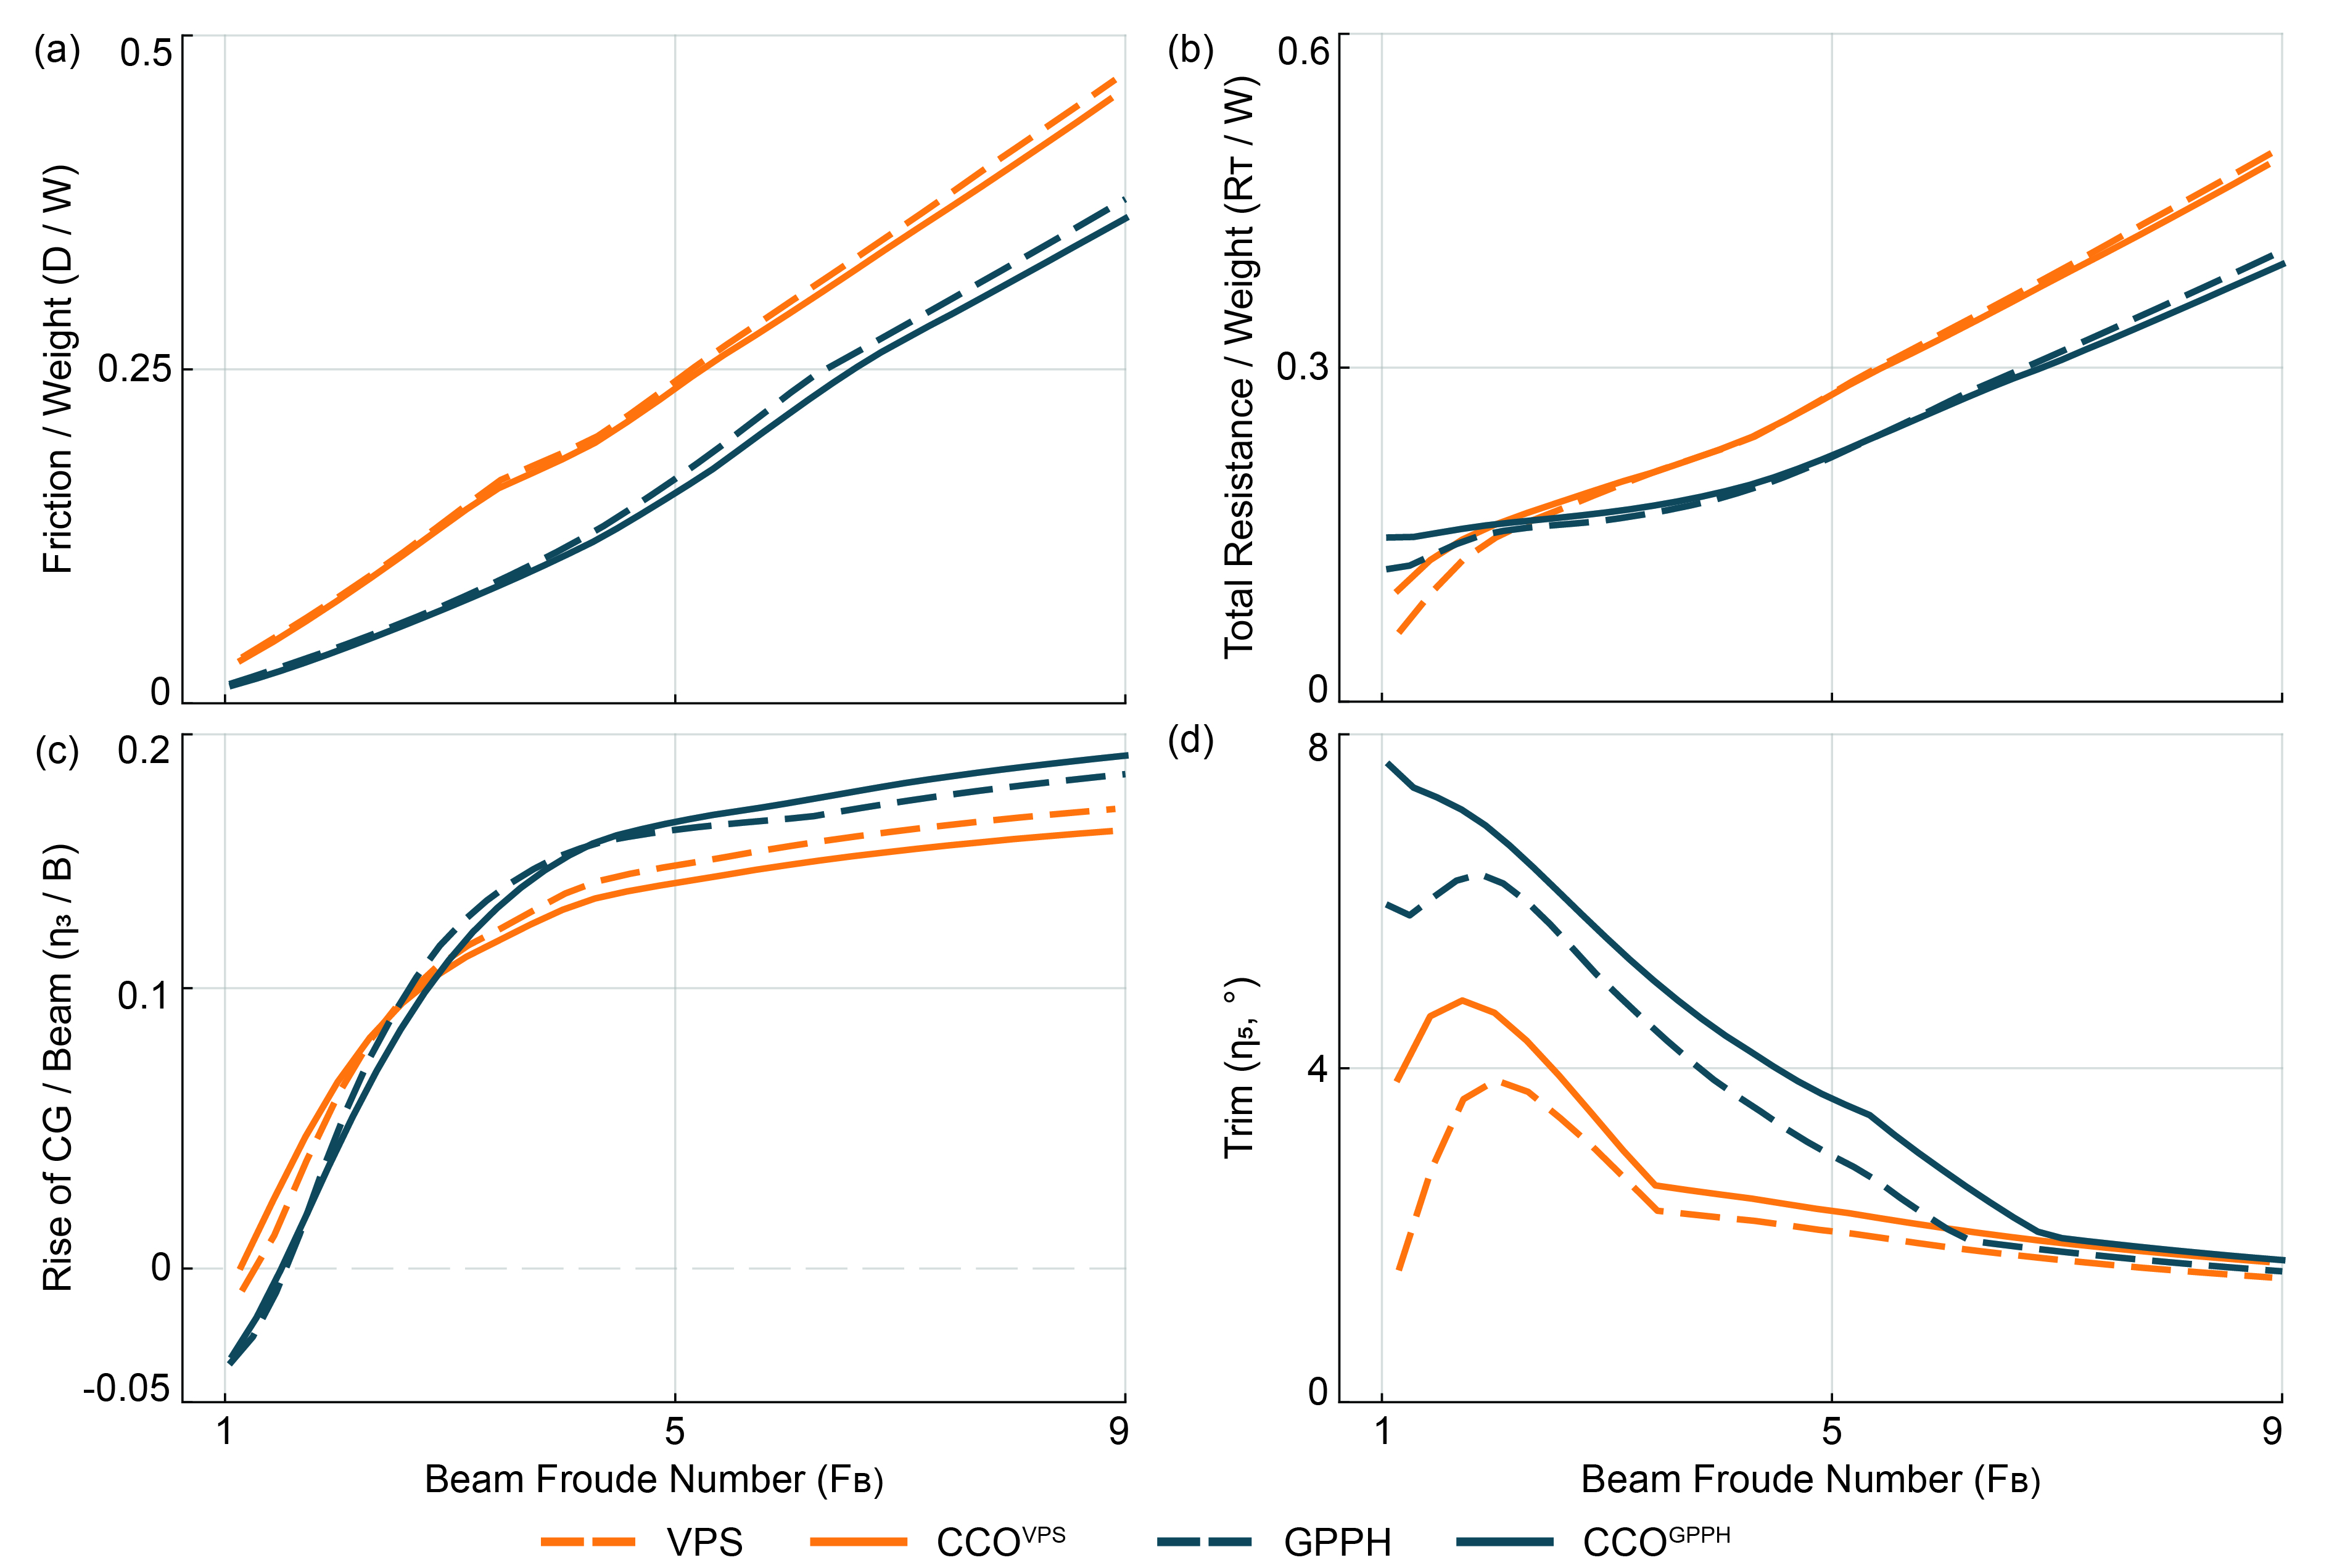
\includegraphics[width=\textwidth]{01-figures/05-04-calm-cco-eval.jpg}
  \caption{Comparison of VPS and GPPH hydrodynamics with their CCO counterparts in calm water: (a) Weight normalized friction drag; (b) Weight normalized total resistance; (c) Beam normalized rise of CG; and (d) Trim angle (positive bow up)}\label{fig-calm-cco-eval}
\end{figure}

It is essential to note that the comparative analysis of CCO hulls with counterparts GPPH and VPS hulls reveals a consistent trend across various hydrodynamic characteristics. Both friction drag in Fig.~\ref{fig-calm-cco-eval}\,(a) and total resistance in Fig.~\ref{fig-calm-cco-eval}\,(b) exhibit a monotonically increasing trend as the planing speed increases. Additionally, the hull tends to rise on the water surface with an increase in planing speed, as evidenced by the rise in CG illustrated in Fig.~\ref{fig-calm-cco-eval}\,(c). Contrarily, the trim angle of the hull diminishes with an increase in the planing speed, as indicated in Fig.~\ref{fig-calm-cco-eval}\,(d). However, it is also imperative to acknowledge a slight disparity in the trim angle of the CCO hulls and their GPPH and VPS counterparts. The following reasons can explain this disparity. First, despite exhibiting a close match, the CCO hulls are not identical in shape to their GPPH and VPS counterparts. The minor differences in the shapes of planing surfaces and beam widths, as documented in Section~\ref{05-subsec-shape-matching} and Table~\ref{tab-cco-hull-geom}, respectively, explain the deviations observed in sinkage and the trim angle at various speeds. Second, Powersea requires the forward perpendicular (FP) to be set at the intersection of the chine and keel lines along the hull's length. For both CCO\(^\textrm{GPPH}\) and GPPH, this requirement results in differing hull length (\(L_{PP}\)) between the aft perpendicular (AP) and the forward perpendicular (FP), as shown in Fig.~\ref{fig-shape-matching}\,(d). Furthermore, Powersea only utilizes the portion of the hull geometry between the AP and FP to simulate its behaviour in water. To ensure consistency across all simulations, we align the FP for all hull geometries with the origin at time t=0. Specifically for the GPPH, the LCG and K\(_{yy}\) are set based on the modeled length of the hull which corresponds to (\(L_{PP}\)) rather than (\(L_{OA}\)) (see Table~\ref{tab-cco-hull-geom}), resulting in a slightly different LCG location compared to CCO\(^\textrm{GPPH}\). These modeling differences lead to varying initial equilibrium positions of the hulls and, consequently, to the differences in the trim angle at various speeds. Lastly, the assumptions in Powersea's underlying theory make it less accurate for predicting hull motion in semi-planing regimes and when the beam Froude numbers are less than or equal to 1. Therefore, the significant deviation in the trim angle at lower speeds can be safely disregarded. At high speeds, when the hulls are advancing in the planing regime, and the bows of the hulls are no longer in contact with the water, the CCO hulls and their counterparts exhibit similar performance.

\begin{figure}[!htbp]
  \centering
  \includegraphics[width=\textwidth]{01-figures/05-05-wavy-cco-eval.jpg}
  \caption{(a) Regular wave characteristics from a nominal Sea Water Level (SWL); (b) Overall length of the boat; Comparison of mean subtracted VPS and GPPH hull motion time histories with their CCO counterparts in head seas: (c) Six seconds of steady state time history for \(\lambda\)/\(L_{OA}\) = 4; (d) Phase shifted steady state time history over 2 second interval for \(\lambda\)/\(L_{OA}\) = 4; (e) Six seconds of steady state time history for \(\lambda\)/\(L_{OA}\) = 10; and (f) Phase shifted steady state time history over two second interval for \(\lambda\)/\(L_{OA}\) = 10. \(\eta_3 / \textrm{\sffamily{A}}\) is heave normalized by wave amplitude.\,\(\eta_5 / \textrm{\sffamily{kA}}\) is pitch normalized by wave slope.}
  \label{fig-wavy-cco-eval}
\end{figure}

The investigation of hull motion in waves is carried out under constant speed, corresponding to a beam Froude number, \(F_B = 4\) when navigating head seas. For VPS and CCO\(^\textrm{VPS}\) hulls, the speed equals 7~m/s, whereas for GPPH and CCO\(^\textrm{GPPH}\) hulls, the speed equals 10~m/s. Wave amplitudes of 0.02~m were applied to the VPS and CCO\(^\textrm{VPS}\) hulls, based on the tank test parameters for VPS hull from the \cite{kim_design_2013} study. The GPPH and CCO\(^\textrm{GPPH}\) hulls were subjected to wave amplitudes of 0.04~m to maintain a wave amplitude to hull length ratio similar to that of the VPS and CCO\(^\textrm{VPS}\) hulls. Each of the four hull geometries was subjected to regular waves with wavelengths, \(\lambda\) equivalent to 4 and 10 times the overall length, \(L_{OA}\) of the planing hull. The graphical representation of these regular wave characteristics is provided in Fig.~\ref{fig-wavy-cco-eval}\,(a-b). Figure~\ref{fig-wavy-cco-eval}\,(c) and~(e) display the final 6~seconds of the 100-second long time histories depicting the steady state, mean-subtracted heave (normalized by wave amplitude) and pitch (normalized by wave slope) motions of the hulls, corresponding to the non-dimensionalized wavelength represented as \(\lambda / L_{OA}\) ratios of 4 and 10, respectively. The mean values of normalized heave and pitch time histories for all hull geometries and \(\lambda / L_{OA}\) ratios are presented in Table~\ref{tab-mean-time-hist}. The small differences in the mean values stem from the variations in hull geometry and the modeling methods, as outlined earlier.

\begin{table}[h!]
  \caption{Mean values of the normalized heave and pitch from Fig.~\ref{fig-wavy-cco-eval}}
  \vspace{-1.5em}
  \begin{center}
	\begin{tabularx}{\textwidth}{ >{\raggedright\arraybackslash}X >{\centering\arraybackslash}m{1in} >{\centering\arraybackslash}m{1in} >{\centering\arraybackslash}m{1in} >{\centering\arraybackslash}m{1in}}
  	\hline
  	\multirow{2}{2.5in}{\textbf{Hull geometry}} & \multicolumn{2}{c}{\textbf{Mean heave, }\(\mathbf{\overline{\bm \eta_3} / A}\)} & \multicolumn{2}{c}{\textbf{Mean pitch, }\(\mathbf{\overline{\bm \eta_5} / kA}\)}\\
  	& \(\lambda/L_{OA} = 4\) & \(\lambda/L_{OA} = 10\) & \(\lambda/L_{OA} = 4\) & \(\lambda/L_{OA} = 10\)\\
  	\hline
    \noalign{\vskip 3pt}
  	CCO\(^\textrm{VPS}\) & 2.846 & 2.127 & 2.252 & 3.354\\  
  	VPS & 2.807 & 2.199 & 1.933 & 2.988\\
  	CCO\(^\textrm{GPPH}\) & 2.085 & 2.273 & 2.741 & 6.778\\  
  	GPPH & 2.788 & 2.494 & 2.854 & 5.939\\
  	\hline
	\end{tabularx}
  \end{center}\label{tab-mean-time-hist}
  \vspace{-1em}
\end{table}

The primary objective of these simulations was to acquire a deeper understanding of the similarities and differences in the hull motion of CCO hulls and their counterparts when subjected to waves. It is observed that the oscillatory hull motion for the GPPH and CCO\(^\textrm{GPPH}\) exhibits a significant phase shift. Nevertheless, the amplitudes and frequencies of the motion are nearly identical when evaluating the mean and phase-shifted data in Fig.~\ref{fig-wavy-cco-eval}\,(d) and~(f). This phase shift in hull motion can be explained by the modeling differences arising from the variations in \(L_{PP}\) and keel configurations between the GPPH and CCO\(^\textrm{GPPH}\) hull designs. In Powersea, the initial wave trough is positioned at the origin and coincides with the hull's FP at time t=0. Because the \(L_{PP}\) differs between the GPPH and CCO\(^\textrm{GPPH}\), the LCG is located differently along each hull's length. This difference results in varying initial equilibrium positions and causes the hulls to encounter waves at different times at the same longitudinal position along the hull. The CCO\(^\textrm{GPPH}\) has an initial draft of 0.153~m and an initial trim of 4.389\(^\circ\). On the other hand, the GPPH has an initial draft of 0.150~m and an initial trim of 3.862\(^\circ\). Thus, the combined effects of the bow shape influencing the initiation of motion in wavy conditions, the differing initial equilibrium position of the hulls, and the time difference in wave encountered at the same longitudinal position along the hulls' length explain the phase shift between the motion histories of GPPH and CCO\(^{\textrm{GPPH}}\) hulls.

In contrast, for the VPS and CCO\(^\textrm{VPS}\) hulls, we observe no phase shift and nearly identical amplitude and frequency of the motion response for both \(\lambda\)/\(L_{OA}\) ratios, as shown in Fig.~\ref{fig-wavy-cco-eval}\,(c-f). It is important to note that for the \(\lambda\)/\(L_{OA}\) ratio of 4, high amplitudes of heave and pitch motion are observed in all four hull geometries, indicating that a wave with \(\lambda\)/\(L_{OA}\) ratio of 4 excites the hulls more than a wave with \(\lambda\)/\(L_{OA}\) ratio of 10.

The findings from this section offer substantial evidence supporting the ability of CCO hulls to emulate the performance of their target hull shapes in both still and wavy water conditions.

\section{Tunable Hydrodynamics With Shape-morphing Curved-origami Hulls}\label{05-sec-tunable-hydrodynamics}
The curved-crease origami planing hull undergoes a gradual transformation from a flat sheet into the characteristic planing hull shape throughout its deployment. By controlling the resting angle of the fold lines located along the chine and keel of the curved-crease origami hull, we gain the ability to morph the hull shape on demand. This ability allows us to change the hull deadrise and grants control over various other geometric attributes, such as the overall length, beam width, bow curvature, center of gravity location, and the radius of gyration. These parameters collectively exert a significant influence on the hydrodynamic characteristics, allowing for on-demand shape morphing and tunability of hull hydrodynamics.

Here, we first discuss the influence of the rest angle of the fold lines on the hull deadrise and the overall hull geometry, which subsequently affects the hydrodynamic behavior. We will study three distinct hull configurations, all obtained from a single curved-crease pattern (starting configuration of flat sheets). As a starting point, we use the same curved-crease pattern as that developed for the VPS hull. The specific folded configurations correspond to deadrise angles of 10\(^\circ\), 20\(^\circ\), and 30\(^\circ\) respectively, as graphically depicted in Fig.~\ref{fig-calm-hydro}. A noticeable trend emerges as the hull's deadrise undergoes a transition from 10\(^\circ\) to 30\(^\circ\). Specifically, this transition is marked by the following changes: an increase in the hull's overall length, a decrease in the beam width, a reduction in the bow's curvature, a forward displacement and vertical ascent of the center of gravity, along with an accompanying increase in the radius of gyration. In order to assess the influence of this morphable hull shape on the hull's hydrodynamic behavior, a series of simulations were conducted using the Powersea software in both calm waters and head seas. The geometric parameters that served as an input for these simulations corresponding to each configuration are presented in Table~\ref{tab-cco-deadrise-geom}.
\begin{table}[h!]
  \caption{Geometric parameters of the variable deadrise CCO hulls for hydrodynamic simulations}
  \vspace{-1.5em}
  \begin{center}
    \begin{tabularx}{\textwidth}{ >{\raggedright\arraybackslash}X >{\centering\arraybackslash}m{0.4in} >{\centering\arraybackslash}m{0.4in} >{\centering\arraybackslash}m{0.6in} >{\centering\arraybackslash}m{0.7in} >{\centering\arraybackslash}m{0.6in} >{\centering\arraybackslash}m{0.7in} >{\centering\arraybackslash}m{0.5in}}
      \hline
      \multirow{2}{3.5in}{\textbf{Hull geometry}\\(deadrise)} & \textbf{L$_{OA}$} & \textbf{L$_{PP}$} & \textbf{LCG } & \textbf{VCG} & \textbf{K$_{yy}$} & \textbf{Weight} & \textbf{B}\\
      & (m)& (m) & (\% L$_{OA}$) & (m) & (m) & (N) & (m)\\
      \hline
      \noalign{\vskip 2pt}
      10\(^\circ\) & 0.889 & 0.879 & 58.76 & 0.08 & 0.574 & 89.3 & 0.319\\
      20\(^\circ\) & 0.945 & 0.935 & 60.53 & 0.096 & 0.623 & 89.3 & 0.304\\
      30\(^\circ\) & 0.962 & 0.952 & 61.12 & 0.097 & 0.639 & 89.3 & 0.278\\
      \hline
    \end{tabularx}
  \end{center}\label{tab-cco-deadrise-geom}
  \vspace{-1em}
\end{table}

\subsection{Calm Water Hydrodynamics}\label{05-subsec-calm-hydro}
The simulations in still water for all three curved-crease origami hull configurations are conducted for various constant speed cases. The speeds (2 to 15.5~m/s) correspond to beam Froude numbers, \(F_B\) ranging from 1 to 9 for each of the three hull geometries. All simulation parameters adhere to the default values specified by Powersea, and the hydrodynamic characteristics are presented in Fig.~\ref{fig-calm-hydro}. Similar to the preceding hydrodynamic investigation conducted in calm water, the attributes studied within this context include: \mbox{(\textit{i}\hspace{.5pt})} friction drag normalized by the hull weight, \mbox{(\textit{ii}\hspace{.5pt})} total resistance normalized by the hull weight, \mbox{(\textit{iii}\hspace{.5pt})} rise of CG normalized by the beam width, and \mbox{(\textit{iv}\hspace{.5pt})} trim angle of the hull.

\begin{figure}[!htbp]
  \centering
  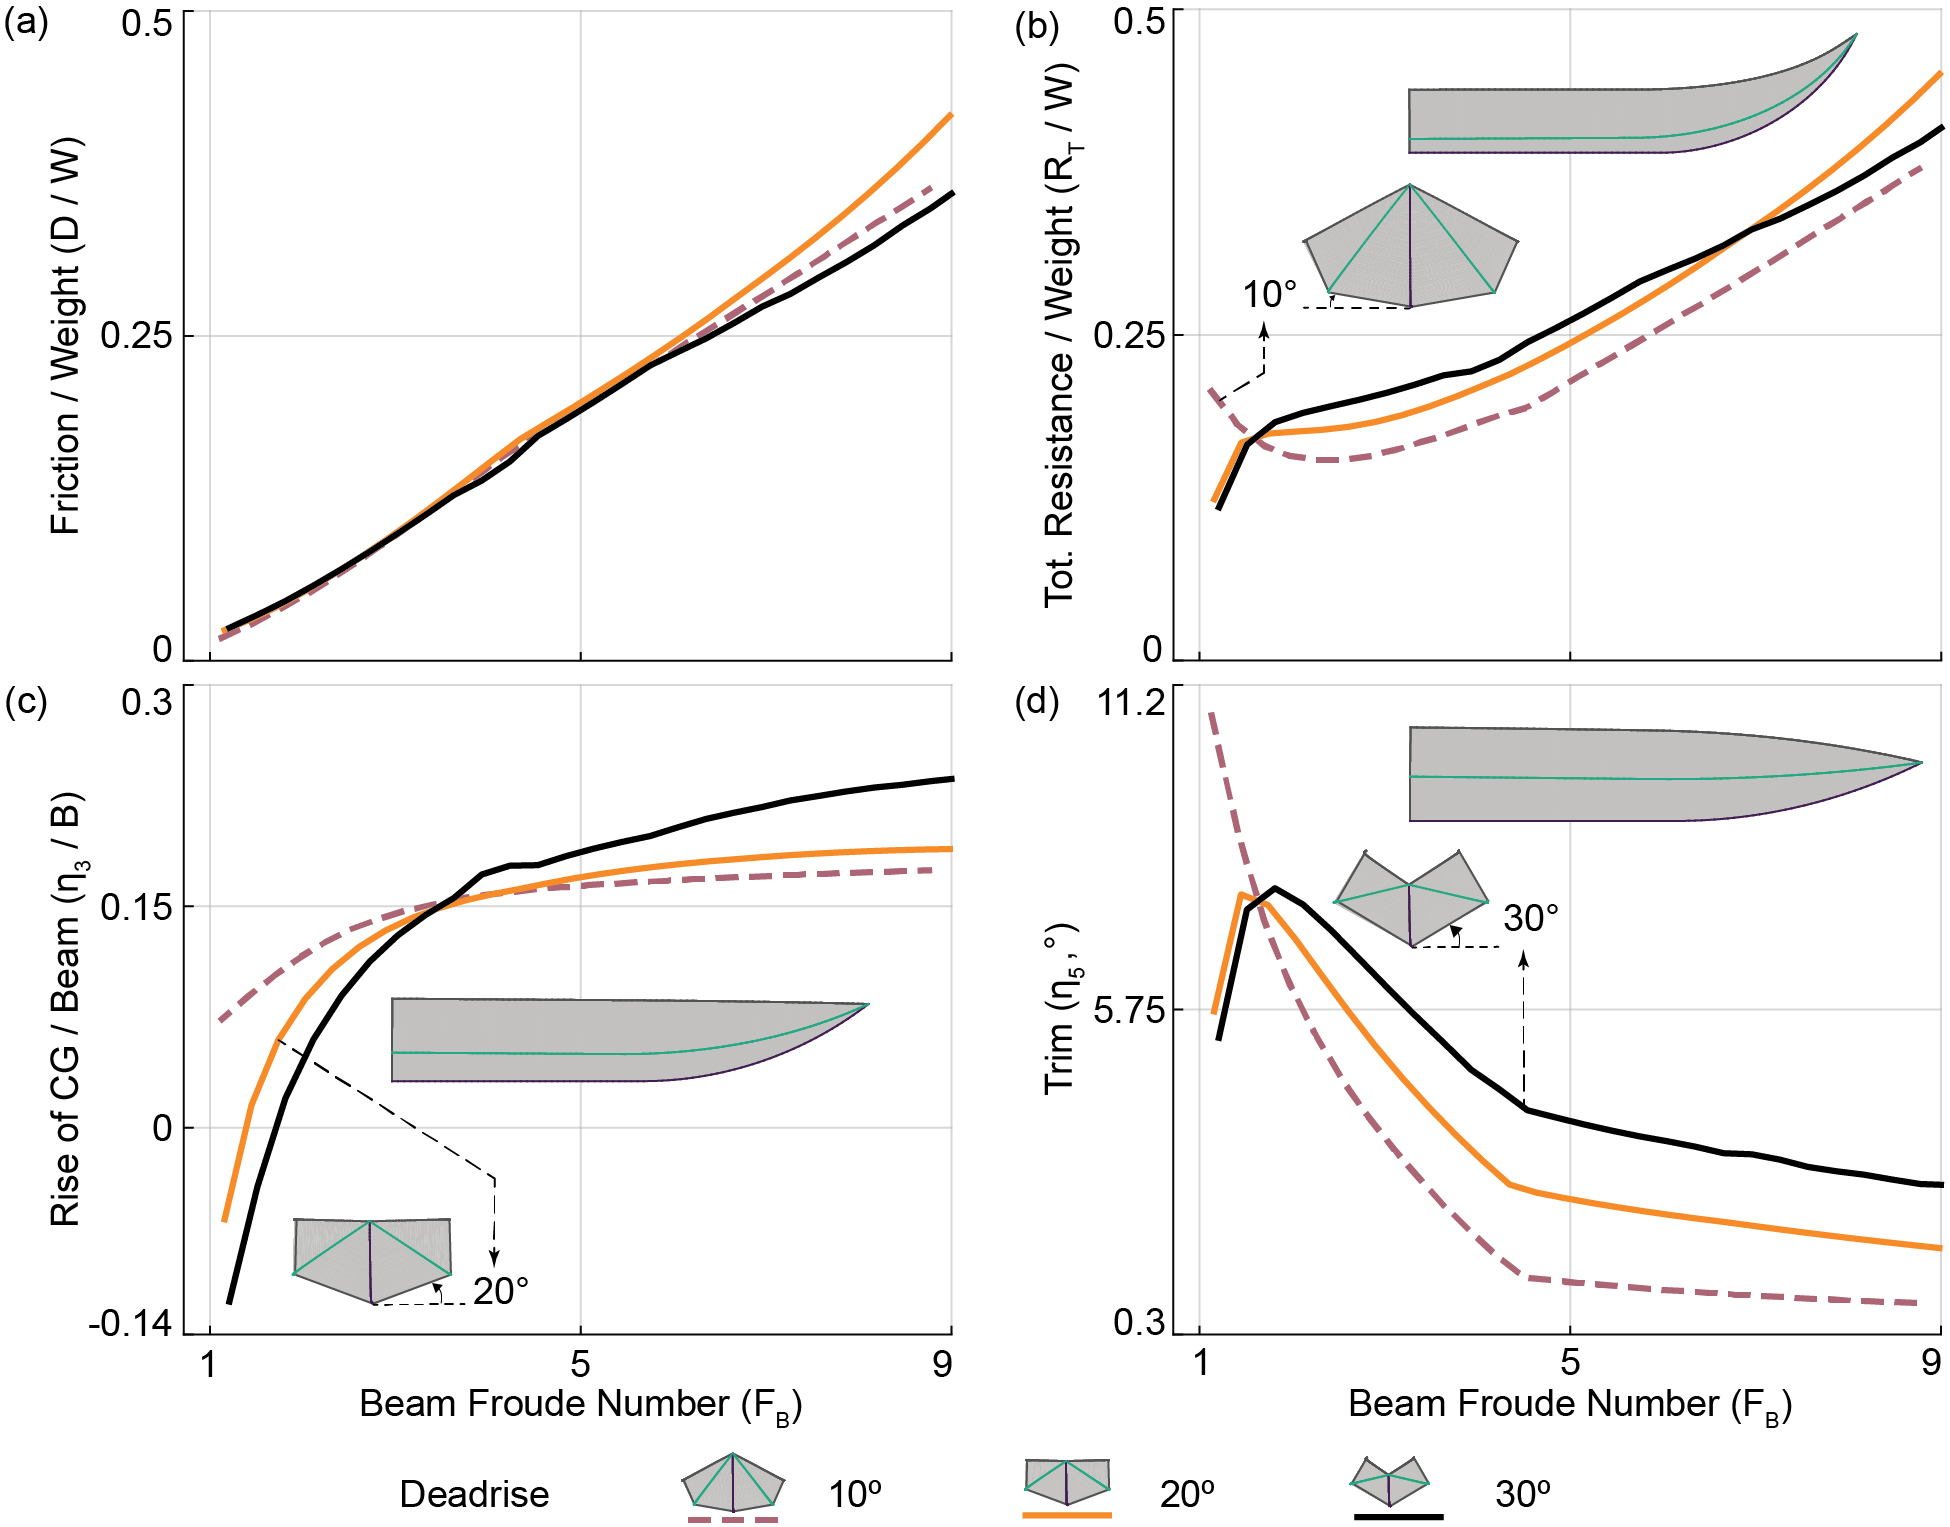
\includegraphics[width=\textwidth]{01-figures/05-06-tunable-calm-hydrodynamics.jpg}
  \caption[]{Effect of varying the CCO hull's deadrise on hydrodynamic performance in calm water: (a) Weight normalized friction drag; (b) Weight normalized total resistance; (c) Beam normalized rise of CG; (d) Trim angle (positive bow up).}
  \label{fig-calm-hydro}
\end{figure}

The influence of shape change on the weight-normalized friction drag experienced by the hull across all deadrise variations is insignificant, except at very high speeds. As illustrated in Fig.~\ref{fig-calm-hydro}\,(a), the 20\(^\circ\) deadrise hull exhibits slightly higher frictional resistance than 10\(^\circ\) and 30\(^\circ\) deadrise configurations at \(F_B\) close to 9. For a lower deadrise configuration, there is an increase in the total resistance at lower speeds, but an interesting reversal of trends emerges at higher speeds. As seen in Fig.~\ref{fig-calm-hydro}\,(b), the lower deadrise configuration now exhibits lower total resistance. A similar trend is also observed for the trim angle of the hull, as shown in Fig.~\ref{fig-calm-hydro}\,(d). This change in trends for total resistance is expected because it is a derived quantity that depends upon the friction drag and trim angle. Since friction drag shows little variation across deadrise configurations, the trend of trim angle contributes to that of the total resistance. In the case of rise of CG, the low deadrise configuration tends to rise higher than the high deadrise configurations for \(F_B\) up to 4, as shown in Fig.~\ref{fig-calm-hydro}\,(c). A noticeable reversal in the hull rise trend emerges at high speeds. The variation in hull rise remains negligible across all deadrise configurations for practical considerations with the exception of the 30\(^\circ\) deadrise configuration. These results can be interpreted in the following ways. In the case of a curved-crease origami hull configured with a lower deadrise, the planing surface typically takes on a flatter and broader profile. Consequently, with increasing surge speed, the hull tends to rise and glide over the water's surface. This phenomenon results in a reduced trim angle as the hull does not have to plow through the water, thereby leading to lower total resistance. In contrast, for a curved-crease origami hull configured with a higher deadrise, the planing surface is generally a shaper V-shape with a narrower profile. This hull tends to sink deeper into the water. Consequently, this hull has to overcome greater total resistance and exhibits increased trim angle at higher surge speeds.

\subsection{Wavy Water Hydrodynamics}\label{05-subsec-wavy-hydro}
The investigation of hull motion in waves is carried out under the condition of a constant speed of 4.04~m/s when navigating head seas. The speed corresponds to \(F_B\) of 2.28, 2.34, and 2.44 for the 10\(^{\circ}\), 20\(^{\circ}\), and 30\(^{\circ}\) deadrise configuration, respectively. Wave amplitudes of 0.02~m are applied to all three hull geometries. Each of the three hull geometries is subjected to regular waves with wavelengths equivalent to 4, 8, and 12 times the overall length of the planing hull. The mean subtracted steady-state hull motion is depicted in Fig.~\ref{fig-wavy-hydro}\,(a-c). These figures display the final 10 seconds of the 100-second time histories and illustrate the heave normalized by wave amplitude and pitch normalized by wave slope of the hulls for the three \(\lambda\)/\(L_{OA}\) ratios.

\begin{figure}[!htbp]
  \centering
  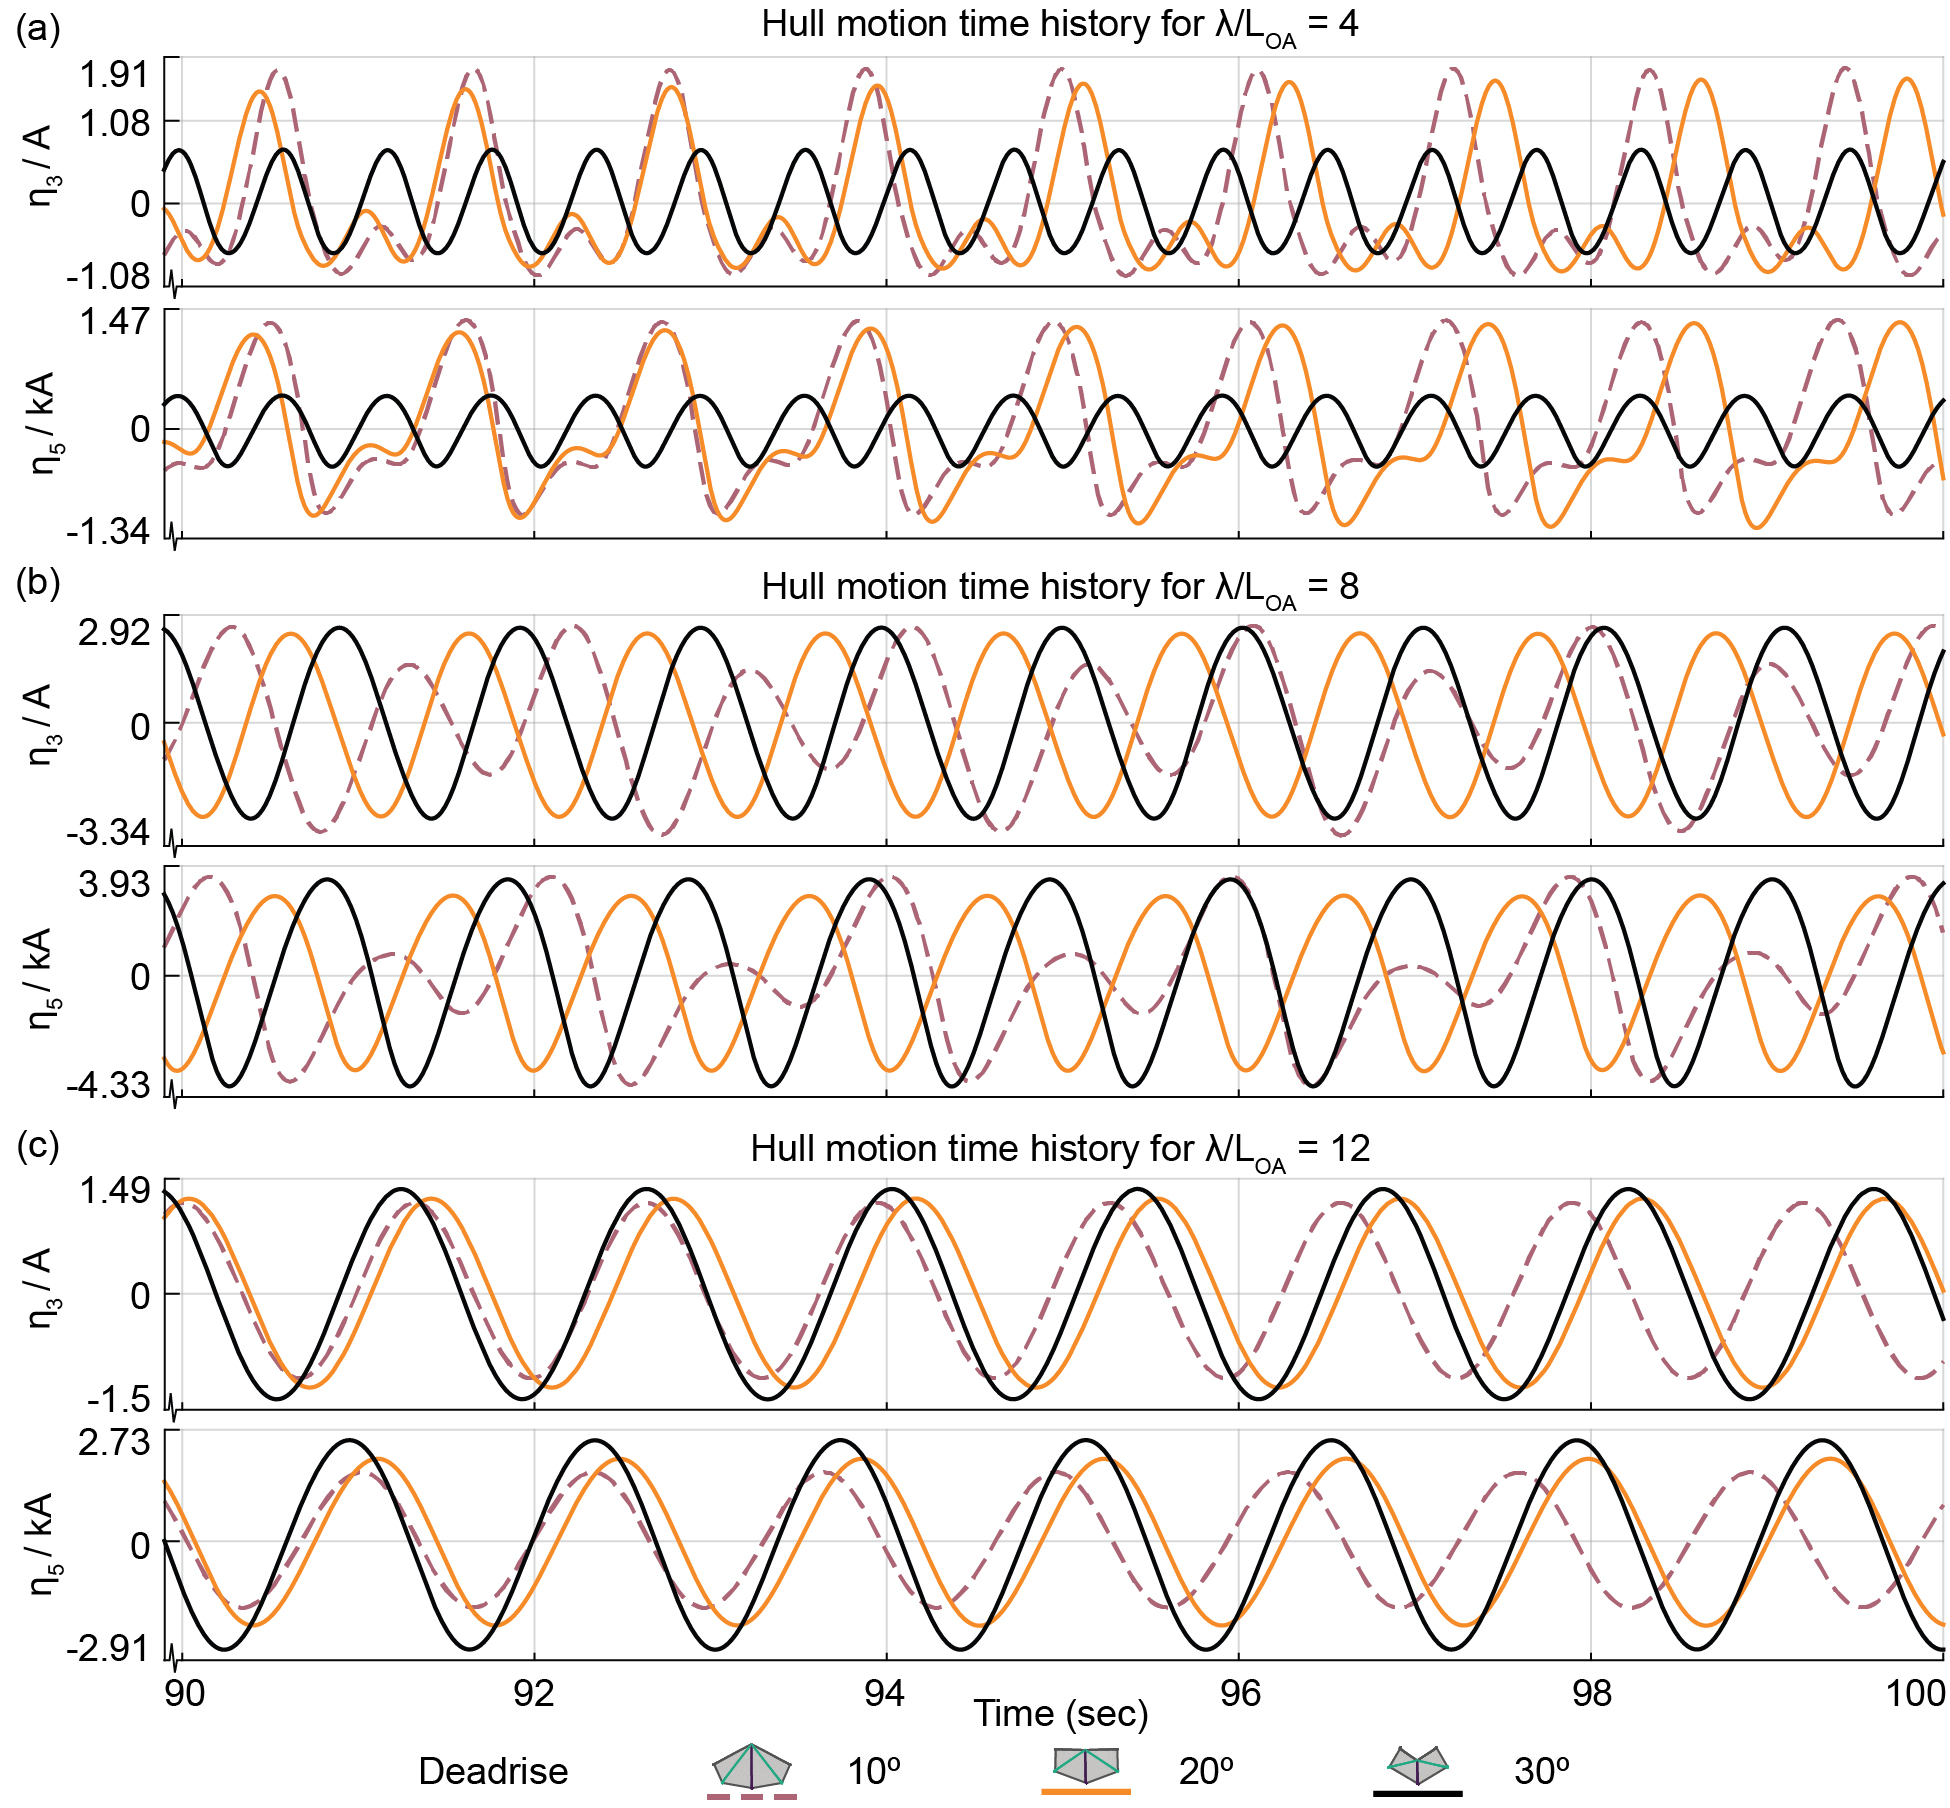
\includegraphics[width=\textwidth]{01-figures/05-07-tunable-wavy-hydrodynamics.jpg}
  \caption{Effect of varying the CCO hull's deadrise on steady state hull motion in head seas for: (a) \(\lambda/L_{OA}\) = 4; (b) \(\lambda/L_{OA}\) = 8; (c) \(\lambda/L_{OA}\) = 12.
  Surge speed is 4.04~m/s, wave amplitude is 0.02~m and the last 10 seconds of the mean subtracted hull motion time history is shown.\,\(\eta_3 / \textrm{A}\) is heave normalized by wave amplitude.\,\(\eta_5 / \textrm{kA}\) is pitch normalized by wave slope.}
  \label{fig-wavy-hydro}
\end{figure}

The objective here is to understand the effects of varying deadrise configurations of the curved-crease origami hull on its performance under different wavy conditions. We observe that the hull configured with 30\(^\circ\) deadrise exhibits strikingly smaller heave and pitch amplitudes for the \(\lambda\)/\(L_{OA}\) ratio of 4 compared to other configurations. As the \(\lambda\)/\(L_{OA}\) ratio increases to 8, the heave and pitch amplitudes increase for all hull shapes. Next, at \(\lambda\)/\(L_{OA}\) ratio of 12, there is a decrease in the motion amplitudes. The hull configured with 10\(^\circ\) deadrise exhibits non-monochromatic hull motion, with higher amplitudes at shorter wavelengths, but reduces in amplitude and becomes monochromatic as the exciting wavelength increases. This hull shape has substantially higher amplitudes at shorter wave frequencies (i.e.~\(\lambda\)/\(L_{OA}\) = 4), which can be expected for planing hulls with lower deadrise angles (flatter hull surface). Our observation here underscores the profound implications of altering the curved-crease origami hull's deadrise configuration on hull motion and overall hydrodynamics. Consequently, the shape-morphing ability of the hull can be harnessed to tune the hull response on-demand, making a single hull geometry adaptable to a wide range of sea conditions.

\section{Physical Implementation}\label{05-sec-physical-implementation}
Translating these designs into practical, life-sized vessels offers several challenges. Critical consideration must be given to selecting appropriate materials for the panels and the flexible joints to ensure the hull's durability while meeting the demands of the naval industry. A preliminary examination of sheet curvature was conducted to identify suitable material options for curved origami panels. Deforming an initially flat sheet to conform to the curved-crease geometry generates significant bending stresses in the sheet itself. These bending stresses can be used to compute a maximum allowable thickness for the sheet, below which the material would remain elastic. The following formula was used to determine the maximum allowable sheet thickness for a given material to fabricate a curved crease origami hull: \( t = 2 \sigma_y / E \kappa \). Here, \(t\) represents the maximum sheet thickness, \(\sigma_y\) corresponds to the material's yield strength, \(E\) denotes the material's Young's modulus, and \(\kappa\) signifies the maximum sheet curvature, obtained from the Bar and Hinge model for a given length of the curved-crease origami hull. Fig.~\ref{fig-prototype}\,(a) graphically depicts the maximum permissible sheet thickness for various materials, such as Aluminium, Glass fiber-reinforced polymer (GFRP), Polycarbonate, Acrylic, and Polyetherimide (Ultem\textregistered{}). This analysis, thus, serves as a crucial reference point for material selection and design considerations in fabricating the curved-crease origami hull.

\begin{figure}[!htbp]
  \centering
  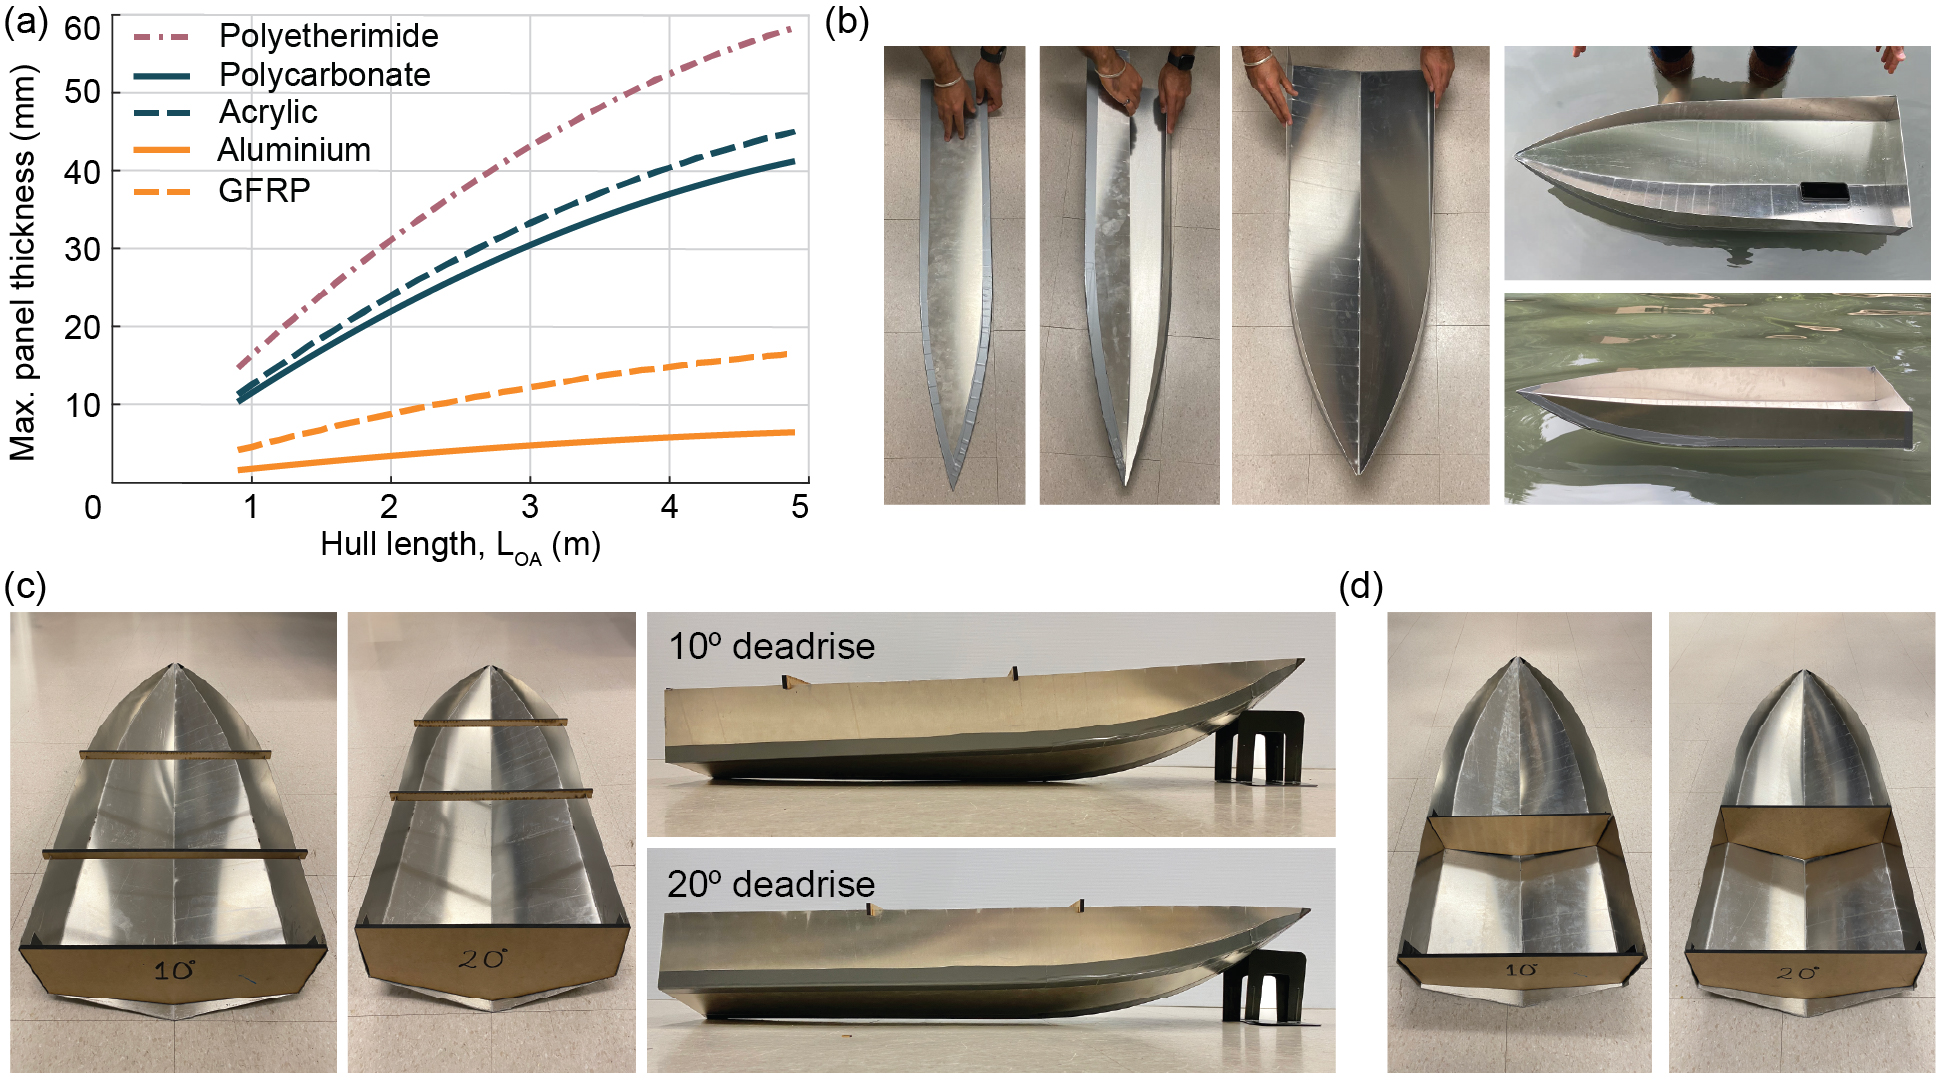
\includegraphics[width=\textwidth]{01-figures/05-08-prototype-scaling-up.jpg}
  \caption{(a) Scalability analysis demonstrating the elastic limit (maximum thickness) for curved-crease origami hulls for different materials; (b) A 91~cm (36~in.) long curved-crease origami hull prototype fabricated using 1.5~mm thick aluminium sheets, joined together with duct tape for flexible joints \textemdash{} displaying the stowed (left) to deployed (right) configuration; (c) Aluminium CCO hull configured with deadrise configurations 10\(^\circ\) and 20\(^\circ\) strengthened with lateral stiffeners that snap onto the side of the hull; (d) Aluminium CCO hulls fitted with solid bulkhead.}
  \label{fig-prototype}
\end{figure}

A scaled model of the curved-crease origami planing hull is constructed by leveraging the results of the curvature analysis. Figure~\ref{fig-prototype}\,(b) showcases a 91~cm (36~inch) long prototype afloat in a water pond, with a smartphone serving as a reference scale. This prototype is constructed using 1.5-millimeter-thick panels of 6061-grade aluminium. The aluminium panels are connected using heavy-duty duct tape along the curved creases, thus serving as the curved-origami fold joints. This prototype serves as an initial proof-of-concept demonstrating the material selection for prototypes to remain elastic. While simplistic, the joints of our prototype are watertight and allow for multiple fold-unfold cycles without degradation.

Post-deployment, the curved crease origami hulls require reinforcement to prevent collapse and torsional deformations. In Fig.~\ref{fig-prototype}\,(c), we present the same aluminium CCO hull from Fig.~\ref{fig-prototype}\,(b), but configured with two distinct deadrise angles \textemdash{} 10\(^\circ\) and 20\(^\circ\). Each deadrise configuration is fortified with snap-fit lateral stiffeners, or girders, constructed from a mid-density fibreboard. These stiffeners effectively prevent collapse and provide sufficient reinforcement against torsional deformations, working in conjunction with the stiffness provided by the transom and curved aluminium sheets. The CCO hulls can also be fitted with solid bulkheads, as shown in Fig.~\ref{fig-prototype}\,(d). In the future, the curved-crease origami hulls can be fitted with deployable bulkheads and stiffeners to strengthen the hull post-deployment.

A parallel fabrication effort was led by Jason P. Kelly and Daniel C. Hart at the Naval Surface Warfare Center, Carderock Division (NSWCCD) for a desktop-scale curved-crease origami-based planing hull~\cite{kelly2025desktop}. This fabrication effort focused on the use of commonly available marine-composite material for the panels and flexible fiber-reinforced neoprene rubber for the curved folds to create an 18~in long prototype of an origami planing hull.

\section{Concluding Remarks}\label{05-sec-hull-conclusion}
This chapter introduces a hull fabrication approach based on curved-crease origami (CCO) principles. Employing the Bar and Hinge model for curved-origami folding and the Hausdorff distance metric, we explored the ability of two CCO hull variants to conform to conventional VPS and GPPH hull shapes. Obtaining conforming designs was achieved by optimizing the geometric parameters of the curved-crease pattern. Next, we demonstrated the ability of CCO hulls to emulate the hydrodynamic performance of conventional hull forms in still and wavy water conditions using the Powersea tool. Finally, we explored the shape-morphing ability of CCO hulls, which enables on-demand tunability of hydrodynamic performance to suit diverse sea conditions. Proof-of-concept prototypes are fabricated to demonstrate the feasibility of CCO for creating hulls.
\chapter{Conclusions and Future Work}\label{chapter-06}
This dissertation addressed the challenge of introducing reconfigurability into static structural systems without abandoning the load-bearing function that makes these systems useful. The central premise of the work is that reconfigurability in structural applications cannot be treated solely as a mechanism-design problem; reconfigurability must also be coupled with strength, stability, fabrication constraints, and predictable load transfer. This dissertation considered the inverse problem of starting with established structural forms and systematically introducing mobility, deployability, and programmable mechanical response. This philosophy was pursued through four objectives: developing a framework for transforming static trusses into reconfigurable systems using planar quadrilateral linkage principles; developing computational tools for evaluating the kinematic and mechanical response of the transformed systems; incorporating programmed hinge behavior to enable functional responses such as multistability and reusable energy-management structures; and broadening the framework beyond civil truss systems through curved-crease origami hulls that are offer rapid deployability and tunable hydrodynamic performance. Together, these objectives establish a foundation for the design and analysis of reconfigurable structural systems that can change shape while retaining meaningful structural function across multiple configurations.

\section{Key Contributions of the Dissertation}\label{06-sec-contributions}
The key contributions of this dissertation are summarized below.

\noindent{}\textbf{A framework for transforming static trusses into reconfigurable systems and evaluating their kinematic behavior.}
This dissertation developed a systematic framework for converting static trusses into reconfigurable systems using principles of flat-foldable quadrilateral linkages. The method transforms triangular units of static trusses into quadrilateral linkages by introducing an additional node into selected members. The node location is determined using closed-form expressions, derived for all triangle geometries, that ensure the resulting quadrilateral linkage satisfies the Grashof flat-foldability criterion (Fig.~\ref{fig-node-intro}). These nodes are placed on tensile members so that the transformed truss retains a stable load path and can carry the prescribed design load despite having mobility greater than one. The unit-level node-placement rules are extended to a system-level workflow that selects candidate members based on both the geometry of the triangular units and the corresponding member forces. The workflow applies to most statically determinate trusses with a continuous sequence of triangular units between the top and bottom chords. Its applicability was demonstrated using conventional truss layouts, including Scissor, Fink, and Warren trusses, as well as topology-optimized layouts, including cantilever, L-shaped, and serpentine trusses. A sequential kinematic simulator was also developed to visualize deployment paths and quantify packing performance as the transformed trusses morph through sequential actuation of their kinematic degrees of freedom. The resulting reconfigurable trusses can reduce their convex hull area by up to 93\% and achieve compact storage while preserving the structural role of the original truss topology.

\noindent{}\textbf{Proof-of-concept prototypes to demonstrate structural capacities of reconfigurable trusses.} We validated the feasibility of constructing real-life reconfigurable trusses using our method by fabricating two proof-of-concept prototypes \textemdash{} a 30~cm reconfigurable cantilever truss and a 3~m Warren truss. Both prototypes employ a joint design strategy that distributes truss members in and out of the plane to ensure desired shape-morphing behavior without member contact or overlap. Load testing of the cantilever trusses confirmed that the reconfigurable truss exhibits force-stable behavior and maintains a peak load capacity and structural stiffness comparable to its static counterparts despite having mobility greater than one. The three-meter-long reconfigurable Warren truss weighing 38~kg supported a peak load of 19~kN, demonstrating the structural capacity and scalability of the proposed designs.

\noindent{}\textbf{Computational tools for mechanical analysis of reconfigurable trusses.}
This dissertation developed computational tools for efficient nonlinear analysis of reconfigurable bar-linked structures whose global response is governed by joint rotational stiffness. The Three-Node Torsional Spring (3NTS) element provides a compact way to incorporate torsional springs into truss-like models without introducing rotational degrees of freedom or replacing joints with artificial beam elements. As a result, reconfigurable trusses with torsional springs can be analyzed using the same translational degrees of freedom as conventional truss models, while capturing large-displacement behavior, elastic buckling, and postbuckling response. This formulation provides the mechanical analysis capability needed to move beyond purely kinematic studies and evaluate how hinge stiffness influences force response, stability, and functional reconfiguration.

\noindent{}\textbf{Programmable hinge mechanics for functional reconfigurable trusses.}
This dissertation extended the modeling capabilities of mechanical analysis tools to enable programmable mechanical response in reconfigurable trusses. An enhanced torsional spring law was introduced to bound the admissible rotation of the 3NTS element while preserving its intended linear response range. This law enables the simulation of sequential folding, locking, and load redistribution among the kinematic degrees of freedom of the truss. The framework was further expanded through magnetic multistable and idealized bistable hinge models, which introduce repeated energy barriers, multiple stable rotational states, and snap-through transitions in the reconfigurable trusses. These models show that local hinge behavior can be programmed to achieve a desired global structural response. In particular, reconfigurable trusses can manage impact energy through controlled geometric transformations rather than permanent material damage. This allows the primary members to remain elastic while the structure absorbs external work through recoverable reconfiguration. This capability provides a basis for reusable impact-energy management systems, controlled deployment paths, and intermediate stable configurations relevant to robotic structures, deployable space systems, and support frames for membrane or origami-based systems.

\noindent{}\textbf{Rapidly deployable, shape-morphing curved-origami hulls with tunable hydrodynamic performance.} Curved-crease origami hulls introduced in this dissertation can reproduce the hydrodynamic behavior of conventional planing hulls while also enabling geometry-based performance tuning. Because these hulls can closely conform to conventional hull geometries, their hydrodynamic response closely matches that of their conventional counterparts, including the VPS and GPPH hulls. Hydrodynamic simulations performed in Powersea show nearly equivalent trends in friction drag, total resistance, hull sinkage, and trim over a wide range of forward speeds in still water. In head-sea conditions, the curved-crease origami hulls also show close agreement with conventional hulls in the amplitude and frequency of hull motion time histories. These results indicate that hulls designed using curved-origami principles can preserve important performance characteristics associated with power efficiency, passenger comfort, and operational safety while providing the fabrication, storage, and deployment advantages of origami-based systems. In addition to replicating conventional hull behavior, the curved-crease origami hulls enable on-demand tuning of hydrodynamic performance by controlling the actuation of fold lines along the keel and chine. Changing the folding angle modifies key geometric features of the hull, especially the deadrise angle. Lower-deadrise configurations produce flatter planing surfaces that are better suited for calm water because they generally reduce sinkage, trim, and resistance. However, these configurations can produce larger heave and pitch in waves and are therefore less effective for seakeeping in wavy conditions. Higher-deadrise configurations produce sharper V-shaped planing surfaces that generally increase resistance, sinkage, and trim in still water but reduce heave and pitch amplitudes in waves. A single curved-crease origami hull can therefore transition between different deadrise configurations suited for different sea states, allowing the same structure to balance operational efficiency, passenger comfort, and seakeeping performance through controlled shape morphing.

\section{Considerations for Future Work}\label{06-sec-future-work}
While the reconfigurable trusses and origami-hulls introduced in this work offer exciting avenues for designing shape-morphing structures, several challenges must be overcome before translating these designs into practical structures. Future work can focus on tackling the following challenges:

\noindent{}\textbf{General methods for designing reconfigurable trusses for three-dimensional structures.}
The node-introduction workflow described in Section~\ref{02-subsec-algo} provides an effective method for transforming many two-dimensional statically determinate trusses into reconfigurable systems. However, the current implementation relies on prescribed rules for hinge placement and is best suited to trusses formed by a single sequence of triangular units. These assumptions limit its use for trusses with multiple layers of triangles, repeated triangular patterns, arbitrary polygonal cells, or three-dimensional connectivity. In such cases, introducing a new node can alter the mobility of several adjacent units. An unsuitable node or hinge location can therefore produce incompatible kinematics, reduce packing efficiency, or compromise structural stability. Future work should develop a more general design framework that identifies node locations, bar connectivity, and hinge-placement strategies without relying on case-specific rules. Graph-theoretic methods offer a promising direction for this generalization because trusses can be represented through nodes, edges, and connectivity constraints. Such a framework could identify the structural subgraphs requiring mobility, determine which bars should remain continuous for load transfer, and select hinge locations that preserve compatible deployment. This approach could also support the design of reconfigurable trusses generated by topology optimization, whose final layouts often include irregular connectivity and polygons with more than three sides. More broadly, a graph-based formulation would help extend the present framework from planar trusses to complex two-dimensional and three-dimensional truss systems while maintaining a direct connection between kinematics, load paths, and structural performance.

\noindent{}\textbf{Mitigating structural overlap to optimize packing density.} As the complexity and degrees of freedom for reconfigurable trusses increase, the potential for structural self-overlapping during actuation becomes increasingly evident. This issue is particularly highlighted in the Scissor truss example illustrated in Fig.~\ref{fig-trad-truss}\,(a), where the actuation of the third degree of freedom results in portions of the structure overlapping. Real-life truss structures cannot achieve a compact state without providing special provisions for folding mechanisms. For such structures, it is crucial to understand their spatial movement patterns and identify the degrees of freedom whose actuation triggers a self-overlap. Addressing this challenge necessitates future investigation into varied sequences of degree-of-freedom actuation to mitigate structural overlap. Furthermore, automating the distribution of truss members out of the plane and incorporating additional methods for node placement (compressive members) will enhance the feasibility of reconfigurable structures. These practices can be explored to prevent self-overlapping and optimize the ability of the structure to minimize its footprint after shape transformations.


\noindent{}\textbf{Coupled hydrodynamic and structural evaluation of shape-morphing curved-crease origami hulls}. Future work should evaluate the coupled relationship between shape morphing, hydrodynamic loading, and structural response in curved-crease origami hulls. The shape change of these curved-origami hulls alters the deadrise angle and other geometric and inertial properties, including hull length, bow curvature, beam width, center of gravity, and radius of gyration. These changes can alter the hull surface pressure distribution, wave response, and local impact loads experienced by the hull. This effect is especially important near the bow, where planing hulls can experience high local pressures under wave-impact loading. The structural response must also be assessed because the shell thickness may be limited by the curvature and foldability requirements of the origami geometry, as shown in Fig.~\ref{fig-prototype}\,(a). Future studies should therefore examine how payload, deadrise configuration, and hull geometry influence hydrodynamic pressures, global forces, stresses, and strains. Higher-fidelity computational models can be used for this purpose, including computational fluid dynamics and one-way coupled fluid-structure interaction analyses. These models can evaluate quantities that are not fully captured by simplified planning-hull tools, such as added wave resistance, spray resistance, local accelerations, and pressure variations over the hull surface. The relationship between shape morphing and seakeeping performance can also be studied using response amplitude operators, such as heave and pitch transfer functions, across different wavelengths and hull configurations. These analyses would clarify how changes in the curved-crease origami shape affect resonant behavior, impact loading, and structural demand. Two-tank experiments can further support the computational results by providing pressure, force, motion, and acceleration measurements for selected configurations.

% Appendices
\appendix
\chapter{Sequential kinematic simulation of multi-DOF reconfigurable trusses}\label{apdx-sequential-kinematics}
This section outlines the method for developing a sequential kinematic simulation program (attached as Supplementary Material), which enables the movement of one degree of freedom at a time in any reconfigurable truss generated by the workflow in Section~\ref{subsec-algo}. The reconfigurable trusses in this study consist of two types of units, each with a single degree of freedom (DOF): \mbox{(\textit{i}\hspace{.5pt})} a Grashof quadrilateral linkage; and \mbox{(\textit{ii}\hspace{.5pt})} a unique configuration of a six-bar linkage. The kinematic simulator performs the position analysis of one DOF at a time, while  applying rigid rotation and translation to the structure excluding DOFs that were actuated in previous steps. The position analysis for the two types of units is performed as follows.

\begin{figure}[!htbt]
  \centering
  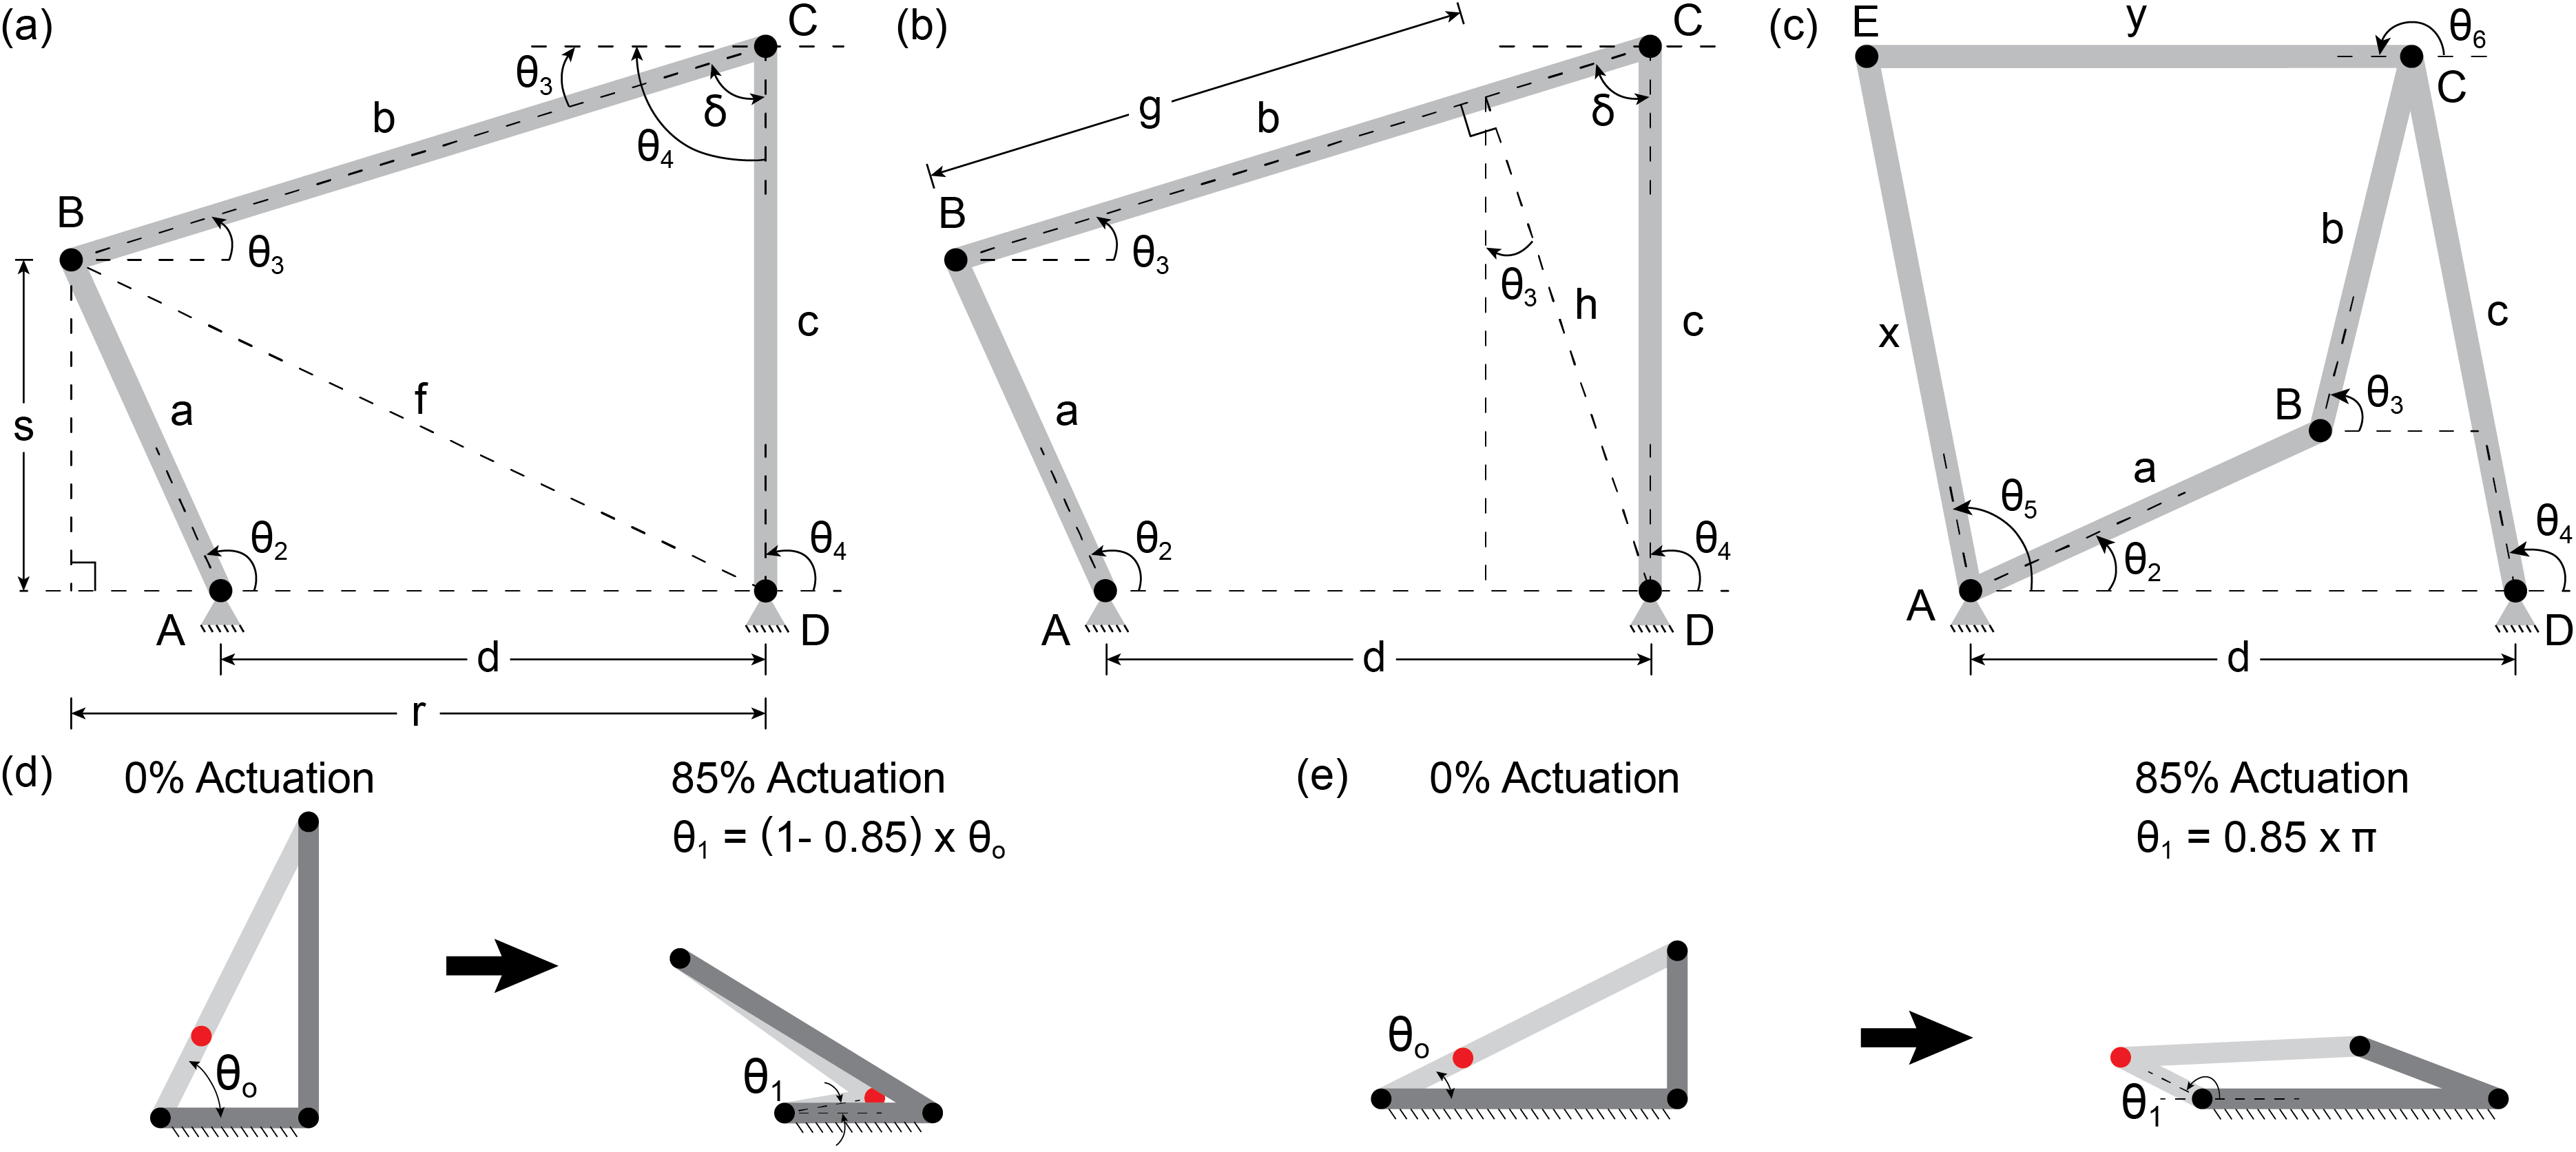
\includegraphics[width=\textwidth]{01-figures/a1-linkage-kinematics-190mm.jpg}
  \caption{Position analysis using the Method of Projections for: (a-b) a general quadrilateral linkage; (c) a unique configuration of a six-bar linkage; (d-e) Extent of actuation in terms of \% actuation of the DOF explained for two different geometries of quadrilateral linkage. \textbf{Note:} A Ground link is not explicitly shown in (a)-(c) but is assumed to be present between nodes A and D.}\label{fig-kinematics}
\end{figure}

\section{Position analysis of a general quadrilateral linkage}\label{apdx-subsec-4bl}
The Method of Projections~\cite[Ch. 4]{constans2018introduction} is used to obtain the position of the nodes of a general quadrilateral linkage, as shown in Fig.~\ref{fig-kinematics}~(a-b). For a general quadrilateral linkage, \(\theta_2\) is the known angle made by the input link \(AB\) of length \(a\). Link \(BC\) is the coupler link of length \(b\) and makes the angle \(\theta_3\) with the horizontal. Link \(CD\) is the output link of length \(c\) and makes the angle \(\theta_4\) with the horizontal. Link \(AD\) is the ground link with length \(d\) and is collinear with the X-axis (horizontal). The objective of the Method of Projection is to find the angles \(\theta_3\), \(\theta_4\), and coordinates of nodes \(B\) and \(C\), given \(\theta_2\), \(a\), \(b\), \(c\), and \(d\).

In Fig.~\ref{fig-kinematics}~(a), \(f\) denotes the prime diagonal of the quadrilateral linkage and \(\delta\) is the angle opposite to \(\theta_2\). The lengths \(r\) and \(s\) are determined using the projections of \(a\) as follows
\begin{flalign}
  \quad r & = d - a\cos{\theta_2}~, &\\
  \quad s & = a\sin{\theta_2}~.
\end{flalign}
Using Pythagoras' Theorem, we note that
\begin{flalign}
  \quad f^2 & = r^2 + s^2~. &\label{eq-pythagoras}
\end{flalign}
From \(\triangle\)BCD, we also have
\begin{flalign}
  \quad f^2      & = b^2 + c^2 - 2bc\cos{\delta}~, &\\\label{eq-cosine}
  \quad \theta_4 & = \theta_3 + \delta~. &
\end{flalign}
Simplifying Eq.~\ref{eq-pythagoras} and Eq.~\ref{eq-cosine} yields
\begin{flalign}
  \quad \delta & = \cos^{-1}{\left(\frac{b^2 + c^2 - r^2 - s^2}{2bc}\right)}~. &
\end{flalign}
\\
Now consider the same quadrilateral linkage, as shown in Fig.~\ref{fig-kinematics}~(b). Here, we use \(\delta\) and projections of \(c\) to find the lengths \(g\) and \(h\) as follows
\begin{flalign}
  \quad h & = c\sin{\delta}~,     &\\
  \quad g & = b - c\cos{\delta}~. &
\end{flalign}
Expressing \(r\) and \(s\) in terms of \(h\) and \(g\), we get
\begin{flalign}
  \quad r & = g\cos{\theta_3} + h\sin{\theta_3}~, &\notag{}\\
  \quad s & = h\cos{\theta_3} -g\sin{\theta_3}~.  &
\end{flalign}
Simplifying further yields
\begin{flalign}
  \quad \theta_3 & = \tan^{-1}\left(\frac{hr - gs}{gr + hs}\right)~. &
\end{flalign}
With \(\theta_3\) known, we can now calculate \(\theta_4\), giving us sufficient information to determine the coordinates of each node relative to \(A\) (or the local origin) as well as use \(\theta_4\) to apply rigid rotation to the remainder of the structure. Points \(A\) and \(D\) remain fixed (as they are the ends of the ground link).
The coordinates of \(B\) are determined as follows
\begin{flalign}
  \quad B_x & = A_x + a \cos{\theta_2}~, &\notag{}\\
  \quad B_y & = A_y + a \sin{\theta_2}~. &
\end{flalign}
Similarly, the coordinates of \(C\) are given by
\begin{flalign}
  \quad C_x & = D_x + c \cos{\theta_4}~, &\notag{}\\
  \quad C_y & = D_y + c \sin{\theta_4}~. &
\end{flalign}

\section{Position analysis of 6 bar linkage with a single degree of freedom}\label{apdx-subsec-6bl}
The second type of unit observed in the reconfigurable trusses of this study is the 6-bar linkage with exactly one degree of freedom, as illustrated in Fig.~\ref{fig-kinematics}~(c). This type of linkage is formed when the two adjacent triangles are congruent and an additional node is introduced on the side shared by the two triangles. In this case, the objective is to find coordinates of \(B\), \(C\), and \(E\), and angles \(\theta_3\), \(\theta_4\), \(\theta_5\), and \(\theta_6\), given \(\theta_2\), \(a\), \(b\), \(c\), \(d\), \(x\), and \(y\).

The analysis to obtain the coordinates of \(B\) and \(C\), and angles \(\theta_3\) and \(\theta_4\) is identical to that performed in Appendix~\ref{apdx-subsec-4bl}. The coordinates of E are obtained by solving the following equations simultaneously, numerically. 
\begin{flalign}
  &\left(E_x - A_x\right)^2 + \left(E_y - A_y\right)^2 - x^2 = 0 &\\
  &\left(E_x - C_x\right)^2 + \left(E_y - C_y\right)^2 - y^2 = 0 &
\end{flalign}
There are two possible solutions for the above equations. We ensure the correctness of the solution by providing an initial guess for the coordinates \(E_x\) and \(E_y\) \textemdash{} coordinate location of \(E\) in the previous step of the simulation. With the coordinates of \(E\) known, we can determine angles \(\theta_5\) and \(\theta_6\). These angles, in addition to the displacement of \(C\) provide us enough information to determine the rigid rotation and translation that must be applied to the remaining structure, depending on the side the structure is connected to.

\section{A note on the extent of actuation of a quadrilateral linkage}\label{apdx-subsec-actuation}
In the sequential kinematic simulator, users can specify the extent of actuation for each DOF. The 0\% actuation state represents the initial configuration, while the 100\% actuation state corresponds to the flat-folded configuration of the quadrilateral linkage. At 0\% actuation of the quadrilateral linkage, the decomposed links of the Candidate link are collinear, as shown in Fig.~\ref{fig-kinematics}\,(d) and (e) on the left side. In this state, \(\theta_o\) represents the angle between the shorter decomposed link and the Ground link. The transition to the flat-folded or 100\% actuation state depends on the geometry of the linkage. The shorter link may rotate in either a clockwise or counterclockwise direction to achieve a flat-folded configuration. In the first case, the shorter link rotates clockwise until it makes an angle of \(0^\circ\) relative to the Ground link. For an intermediate state of 85\% actuation, the shorter link is rotated to an angle of \(\theta_1 = (1 - 0.85)\times\theta_o\) relative to the Ground link as shown in Fig.~\ref{fig-kinematics}\,(d, right). In the second case, the shorter link rotates anti-clockwise until it makes an angle of \(180^\circ\) relative to the Ground link. For an intermediate state of 85\% actuation, the shorter link is rotated to an angle of \(\theta_1 = 0.85\times\pi\) relative to the Ground link, as shown in Fig.~\ref{fig-kinematics}\,(e, right).}
\chapter{Reconfigurable Truss Prototype Load Test Videos}\label{02-appendix-truss-videos}}

% Give this command the relative path to the .bib file.
\nocite{*}
\bibliographystyle{plain}
\bibliography{references}
\end{document}